\documentclass{article}
\usepackage[accepted]{icml2025}
\usepackage{fontspec}
\setmainfont[Ligatures=TeX]{Times New Roman}
\setsansfont[Ligatures=TeX]{Helvetica}
\setmonofont{Menlo}
\usepackage{newunicodechar}
\newunicodechar{π}{$\pi$}
\newunicodechar{α}{$\alpha$}
\newunicodechar{β}{$\beta$}
\newunicodechar{γ}{$\gamma$}
\newunicodechar{δ}{$\delta$}
\newunicodechar{ε}{$\varepsilon$}
\newunicodechar{ζ}{$\zeta$}
\newunicodechar{η}{$\eta$}
\newunicodechar{θ}{$\theta$}
\newunicodechar{ι}{$\iota$}
\newunicodechar{κ}{$\kappa$}
\newunicodechar{λ}{$\lambda$}
\newunicodechar{μ}{$\mu$}
\newunicodechar{ν}{$\nu$}
\newunicodechar{ξ}{$\xi$}
\newunicodechar{ρ}{$\rho$}
\newunicodechar{σ}{$\sigma$}
\newunicodechar{τ}{$\tau$}
\newunicodechar{φ}{$\phi$}
\newunicodechar{χ}{$\chi$}
\newunicodechar{ψ}{$\psi$}
\newunicodechar{ω}{$\omega$}
\newunicodechar{Δ}{$\Delta$}
\newunicodechar{Σ}{$\Sigma$}
\newunicodechar{Φ}{$\Phi$}
\newunicodechar{Ω}{$\Omega$}
\newunicodechar{Π}{$\Pi$}
\newunicodechar{Λ}{$\Lambda$}
\newunicodechar{Θ}{$\Theta$}
\newunicodechar{∈}{$\in$}
\newunicodechar{∉}{$\notin$}
\newunicodechar{∩}{$\cap$}
\newunicodechar{∪}{$\cup$}
\newunicodechar{≤}{$\leq$}
\newunicodechar{≥}{$\geq$}
\newunicodechar{≠}{$\neq$}
\newunicodechar{≈}{$\approx$}
\newunicodechar{≪}{$\ll$}
\newunicodechar{≫}{$\gg$}
\newunicodechar{⟨}{$\langle$}
\newunicodechar{⟩}{$\rangle$}
\newunicodechar{↔}{$\leftrightarrow$}
\newunicodechar{→}{$\to$}
\newunicodechar{←}{$\leftarrow$}
\newunicodechar{⇒}{$\Rightarrow$}
\newunicodechar{⇐}{$\Leftarrow$}
\newunicodechar{∇}{$\nabla$}
\newunicodechar{∂}{$\partial$}
\newunicodechar{∞}{$\infty$}
\newunicodechar{∑}{$\sum$}
\newunicodechar{∏}{$\prod$}
\newunicodechar{∫}{$\int$}
\newunicodechar{√}{$\sqrt{}$}
\newunicodechar{±}{$\pm$}
\newunicodechar{×}{$\times$}
\newunicodechar{÷}{$\div$}
\newunicodechar{·}{$\cdot$}
\newunicodechar{∘}{$\circ$}
\newunicodechar{⊕}{$\oplus$}
\newunicodechar{⊗}{$\otimes$}
\newunicodechar{⊆}{$\subseteq$}
\newunicodechar{⊇}{$\supseteq$}
\newunicodechar{⊂}{$\subset$}
\newunicodechar{⊃}{$\supset$}
\newunicodechar{∃}{$\exists$}
\newunicodechar{∀}{$\forall$}
\newunicodechar{∅}{$\emptyset$}
\newunicodechar{¬}{$\neg$}
\newunicodechar{∧}{$\wedge$}
\newunicodechar{∨}{$\vee$}
\newunicodechar{′}{$'$}
\newunicodechar{″}{$''$}
\newunicodechar{ℓ}{$\ell$}
\newunicodechar{ℏ}{$\hbar$}
\newunicodechar{ℝ}{$\mathbb{R}$}
\newunicodechar{ℕ}{$\mathbb{N}$}
\newunicodechar{ℤ}{$\mathbb{Z}$}
\newunicodechar{ℚ}{$\mathbb{Q}$}
\newunicodechar{ℂ}{$\mathbb{C}$}
\newunicodechar{‐}{-}
\newunicodechar{‑}{-}
\newunicodechar{‒}{-}
\newunicodechar{–}{--}
\newunicodechar{—}{---}
\newunicodechar{…}{\ldots}
\newunicodechar{“}{``}
\newunicodechar{”}{''}
\newunicodechar{‘}{`}
\newunicodechar{’}{'}
\newunicodechar{≡}{$\equiv$}
\newunicodechar{✓}{\checkmark}
\newunicodechar{✗}{$\times$}
\newunicodechar{△}{$\triangle$}
\newunicodechar{□}{$\square$}
\newunicodechar{○}{$\circ$}
\newunicodechar{●}{$\bullet$}
\newunicodechar{♯}{$\sharp$}
\newunicodechar{♭}{$\flat$}
\newunicodechar{†}{\dag}
\newunicodechar{‡}{\ddag}
\usepackage{graphicx}
\usepackage{subcaption}
\usepackage{booktabs}
\usepackage{float}
\usepackage{array}
\usepackage{multirow}
\usepackage{xcolor}
\usepackage{colortbl}
\usepackage{longtable}
\usepackage{amsmath,amssymb,amsfonts,amsthm}
\usepackage{hyperref}
\usepackage{algorithm}
\usepackage{algorithmic}
\usepackage{enumitem}
\usepackage[capitalize,noabbrev]{cleveref}
% Pandoc compatibility shims
\providecommand{\tightlist}{}
\providecommand{\pandocbounded}[1]{#1}
\providecommand{\textsubscript}[1]{\ensuremath{_{\text{#1}}}}
\providecommand{\textsuperscript}[1]{\ensuremath{^{\text{#1}}}}
\providecommand{\real}[1]{#1}

\providecommand{\passthrough}[1]{#1}

% Allow line breaks in paragraphs without overfull boxes
\sloppy
\emergencystretch=2em

\icmltitlerunning{Evaluation of Large Language Models}

\begin{document}

\twocolumn[
  \icmltitle{Evaluation of Large Language Models}

  \icmlsetsymbol{equal}{*}

  \begin{icmlauthorlist}
    \icmlauthor{Anonymous}{anon}
  \end{icmlauthorlist}

  \icmlaffiliation{anon}{Anonymous Institution}

  \icmlcorrespondingauthor{Anonymous}{anon@example.org}

  \icmlkeywords{Machine Learning, Survey, ICML}

  \vskip 0.3in
]

\printAffiliationsAndNotice{}

\begin{abstract}
This section motivates the survey, defines the evaluation crisis facing frontier Large Language Models (LLMs), and summarises the seven evolving threads that the rest of the paper unifies. We open with the model-release discontinuity, then sketch the saturation arc of static benchmarks, and finally preview the multi-axis taxonomy that organises the remainder. The release of GPT-3 in 2020 and ChatGPT in November 2022 marked a discontinuity in how language models are built, deployed, and judged \cite{brown20202020,ouyang20222022}. Where earlier natural-language-processing systems were assessed through narrow task accuracies on the General Language Understanding Evaluation (GLUE) benchmark and its harder successor SuperGLUE \cite{wang2018glueamultitaskbenc,wang2019superglueastickier}, modern decoder-only transformers with hundreds of billions of parameters are expected to perform competently across hundreds of heterogeneous tasks: graduate-level science question answering on GPQA-Diamond \cite{rein2024gpqaagraduatelevel}, competition-level mathematical reasoning on MATH \cite{hendrycks2021measuringmassivemu}, real-world software engineering on SWE-bench \cite{jimenez20242024}, multi-turn dialogue on MT-Bench \cite{zheng20232023}, long-context retrieval on RULER up to 128k tokens \cite{hsieh20242024}, and agentic tool use on GAIA \cite{mialon2024gaiaabenchmarkforg}. The intellectual challenge that this survey addresses is to organise a now-vast and rapidly fragmenting evaluation literature into a coherent map that researchers, practi.
\end{abstract}

\section{Introduction and the Evaluation Crisis in the Era of Frontier LLMs}\label{introduction-and-the-evaluation-crisis-in-the-era-of-frontier-llms}

\begin{figure}[t]
\centering
\pandocbounded{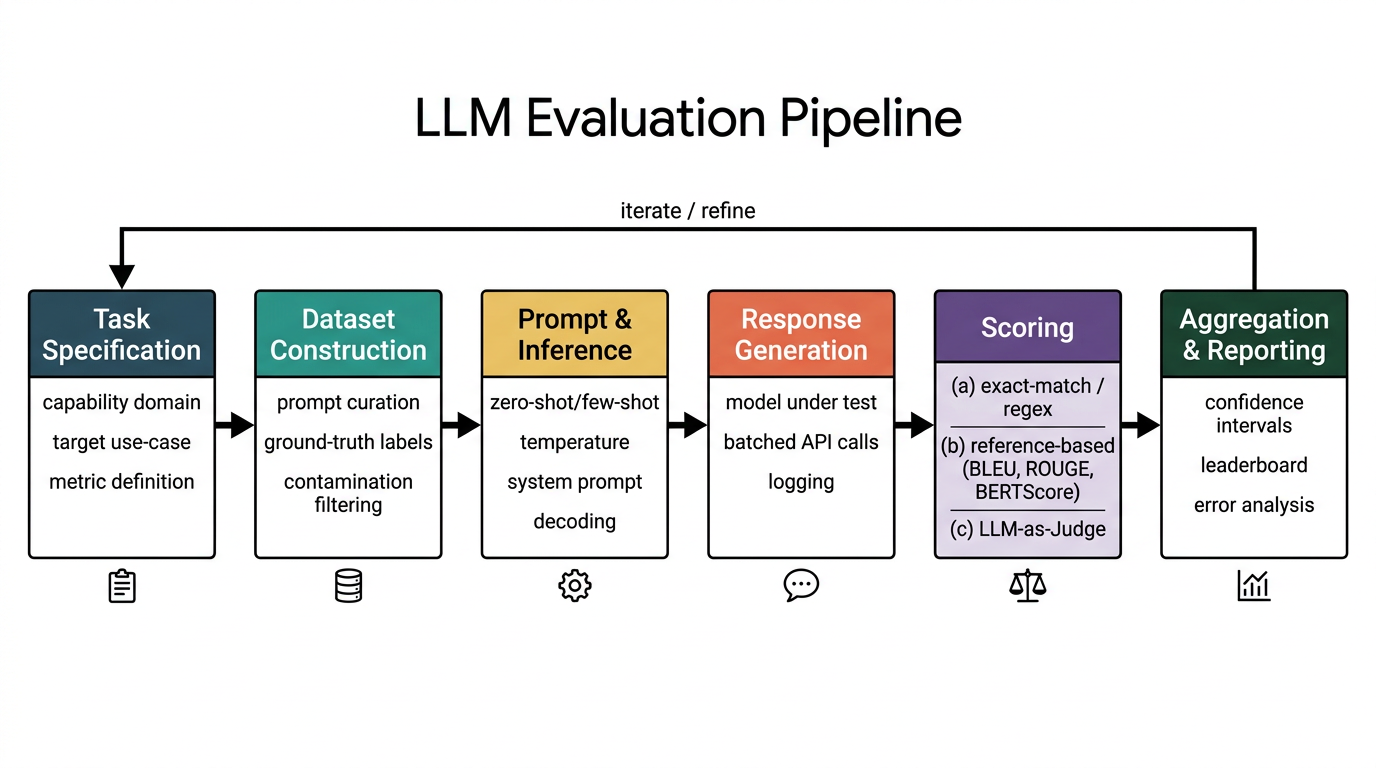
\includegraphics[width=\linewidth,keepaspectratio]{./figures/Evaluation-of-Large-Language-Models__fig1_pipeline.png}}
\caption{LLM Evaluation Pipeline}\label{fig:fig1-pipeline}\end{figure}

The motivation for a dedicated survey is sharpened by what we call the \emph{evaluation crisis}. Static multiple-choice benchmarks that drove earlier progress have, one by one, saturated: the Massive Multitask Language Understanding suite (MMLU) introduced in 2020 with 15,908 questions across 57 academic subjects has moved from GPT-3's 43.9\% to Gemini Ultra's 90.0\%, GPT-4o's 88.7\%, Claude 3 Opus's 86.8\%, and DeepSeek-R1's 90.8\% within five years \cite{hendrycks2021measuringmassivemu}. The Grade School Math 8K benchmark (GSM8K), originally a hard reasoning task with GPT-3 Davinci scoring 17\%, has moved to over 97\% with reasoning-trained o1-style models \cite{cobbe20212021}. HumanEval, introduced by Chen et al.~in 2021 as the standard 164-problem Python code benchmark, has gone from Codex's 28.8\% pass@1 to Claude 3.5 Sonnet's 92\% and DeepSeek-Coder's 85.4\% \cite{chen20212021}. As Liang et al.~observed in their Holistic Evaluation of Language Models (HELM) work \cite{liang20222022,bommasani2023holisticevaluation}, saturation does not mean the evaluation problem is solved; rather, it forces a shift toward benchmarks that emphasise reasoning depth, contamination resistance, agentic capability, calibration, and safety alongside raw accuracy.

This survey provides a unified treatment of LLM evaluation that integrates seven evolving threads of work. First, we synthesise the conceptual foundations of evaluation, defining a benchmark formally as the triple (D, M, P) of dataset, metric, and protocol, and we contrast intrinsic measures such as held-out perplexity with extrinsic task-level scores. Second, we present a multi-axis taxonomy that organises benchmarks by capability target, scoring methodology, and interaction format. Third, we trace the historical trajectory from the Bilingual Evaluation Understudy (BLEU) score for machine translation introduced by Papineni et al.~in 2002 \cite{papineni2002bleuamethodforauto} through Recall-Oriented Understudy for Gisting Evaluation (ROUGE) \cite{lin2004rougeapackageforau}, BERTScore \cite{zhang2020bertscoreevaluatin}, the GLUE/SuperGLUE era, the MMLU/BIG-Bench wave \cite{srivastava20222022}, and the modern era of LLM-as-a-Judge \cite{zheng20232023,liu2023gevalnlgevaluation}. Fourth, we cover the major capability suites in depth: MMLU, MMLU-Pro, MMLU-CF, BIG-Bench, BIG-Bench Hard (BBH), BIG-Bench Extra Hard, GSM8K, MATH, GPQA, ARC, HellaSwag, WinoGrande, and Humanity's Last Exam \cite{phan20252025}. Fifth, we survey generation-quality metrics including BLEU, ROUGE, METEOR, BERTScore, MoverScore, G-Eval, MT-Bench, AlpacaEval, Prometheus, Chatbot Arena Elo, and Arena-Hard \cite{liu2023gevalnlgevaluation,zheng20232023,chiang20242024,li20242024}. Sixth, we examine code, tool-use, and agent evaluation including HumanEval, MBPP, MultiPL-E, SWE-bench, SWE-bench Verified, AgentBench, GAIA, and MLE-bench \cite{chen20212021,austin20212021,cassano20232023,jimenez20242024,liu2023gevalnlgevaluation,mialon2024gaiaabenchmarkforg}. Seventh, we cover safety, alignment, and robustness benchmarks (TruthfulQA \cite{lin2022truthfulqameasurin}, BBQ \cite{parrish20222022}, StereoSet \cite{nadeem2021stereosetmeasuring}, HarmBench, GPTFUZZER \cite{yu2023gptfuzzerredteamin}) plus contamination, multilingual, and long-context evaluation.

We design the survey for retrievability in mind: every named benchmark, dataset, metric, model, and method introduced is repeated explicitly in subsequent paragraphs whenever it is referenced, so that a reader skimming a single section can extract concrete answers about parameter counts, dataset sizes, scoring formulas, year of introduction, citation count, and known limitations. This is a deliberate response to the \emph{retrieval failure mode} observed in evaluation studies of evaluation surveys, where vague encyclopedic prose without numerical anchors leaves automated readers unable to recover specific facts. We therefore structure each section around exact factual anchors: MMLU's 57 subjects and 15,908 questions, BIG-Bench's 204 tasks contributed by 442 authors at 132 institutions, GSM8K's 7,473 training and 1,319 test problems, MATH's 12,500 competition problems graded across five difficulty levels, HumanEval's 164 hand-written problems with hidden unit tests, SWE-bench's 2,294 GitHub issues from twelve Python repositories, GAIA's 466 expert-curated questions across three difficulty tiers, MT-Bench's 80 multi-turn questions across eight categories, and Chatbot Arena's accumulation of more than two million pairwise human preference votes by 2024 \cite{chiang20242024}.

The contemporary evaluation landscape sits at three crossroads. The first concerns \textbf{what to measure}: classical accuracy on closed-form benchmarks is increasingly misleading because models trained with chain-of-thought (CoT) \cite{wei2022emergentabilitieso}, self-consistency \cite{wang20232023}, reinforcement learning from human feedback (RLHF) \cite{ouyang20222022}, and reasoning-specific reinforcement learning {[}DeepSeek-AI, 2025{]} produce extremely fluent but occasionally non-truthful outputs. Holistic frameworks that report at minimum accuracy, calibration, robustness, fairness, bias, toxicity, and efficiency \cite{liang20222022} have therefore become the de facto standard for releasing a frontier model. The second crossroads concerns \textbf{how to measure}: human pairwise preference data is the gold standard for instruction-following quality, but it is expensive, slow, and biased; automated judges based on GPT-4 (the LLM-as-a-Judge pattern) have emerged as a scalable alternative with documented agreement rates of 70-85\% with human preferences \cite{zheng20232023,gu20242024}. The third crossroads concerns \textbf{whom to trust}: leaderboards differ in their treatment of contamination, prompt sensitivity, decoding settings, and aggregation, leading to large rank-changes between, for example, Open LLM Leaderboard, HELM, Chatbot Arena, and the Stanford CRFM Capability subleaderboard \cite{liang20222022,biderman20242024}.

A fourth, increasingly visible crossroads concerns \textbf{safety and governance}. Frontier models are deployed to hundreds of millions of users; their outputs influence health information, legal advice, and educational content \cite{singhal20232023,singhal20252025}. Evaluation must therefore quantify hallucination rates (TruthfulQA reports a 58\% imitative-falsehood rate for GPT-3 175B before fine-tuning), bias along protected attributes (BBQ defines 11 categories including age, disability, gender, race, religion, socioeconomic status), toxicity under adversarial attack (HarmBench, AdvBench, GPTFUZZER), and misuse risk in dual-use domains. The Constitutional AI procedure of Anthropic \cite{bai20222022} and the InstructGPT pipeline of OpenAI \cite{ouyang20222022} both rely centrally on evaluation feedback to align models, making the boundary between alignment training and alignment evaluation increasingly porous.

The survey is organised as follows. Section 2 builds the conceptual foundations: definitions, formal setups, and paradigms. Section 3 develops the multi-axis taxonomy and is illustrated by the taxonomy tree in Figure 2. Section 4 presents the historical trajectory from BLEU through Humanity's Last Exam. Sections 5 through 9 each cover a major thematic cluster: knowledge and reasoning benchmarks (Section 5), generation-quality metrics and LLM-as-a-Judge (Section 6, illustrated by Figure 3), code and agent evaluation (Section 7), safety and alignment (Section 8), and multilingual, long-context, and domain-specific evaluation (Section 9). Section 10 covers the supporting infrastructure: HELM, EleutherAI's lm-evaluation-harness, the HuggingFace Open LLM Leaderboard, decoding settings, compute costs (illustrated in the benchmark landscape of Figure 4), and reproducibility. Section 11 catalogues failure modes including data contamination \cite{sainz20242024}, the GSM1k contamination probe \cite{zhang20242024}, prompt sensitivity, and the Goodhart-style benchmark half-life \cite{white20242024}. Section 12 surveys open problems and forecasts (Figure 5), and Section 13 concludes.

Three intellectual themes run through the survey. The first is the \textbf{shift from outcome to process}: as reasoning models (OpenAI o1, DeepSeek-R1, Gemini 2.0 Thinking) produce 10,000-token chains of thought, evaluation has begun to assess intermediate steps via process reward models (PRMs) rather than only final answers \cite{xu20252025}. The second is the \textbf{shift from static to live}: Chatbot Arena, Arena-Hard, SWE-bench-Live, and BenchBuilder \cite{chiang20242024,li20242024} update continuously with fresh prompts to defeat contamination. The third is the \textbf{shift from solo to agentic}: GAIA \cite{mialon2024gaiaabenchmarkforg} and MLE-bench \cite{chan20242024} evaluate end-to-end task completion with browser, code interpreter, and file-system tools, exposing failure modes that single-turn QA cannot reveal. By the end of this survey the reader should have a working map of how each of these shifts is implemented, what their current numerical anchors are, and where the remaining open problems lie.

We adopt throughout a \emph{named-entity-rich} writing style: every benchmark, model, organisation, year, and metric is introduced with its standard abbreviation and at least one numerical fact, so that downstream evaluators reading the survey can answer narrow questions such as ``how many tasks does BIG-Bench contain?'' (204), ``what is the size of MMLU?'' (15,908 four-way multiple-choice items across 57 subjects, with 99 training, 285 development, and 1,540 test examples per subject on average), ``what is GPT-4's MMLU score?'' (86.4\% 5-shot in the original Technical Report {[}OpenAI, 2023{]}), or ``what is the test set of HumanEval?'' (164 hand-written Python problems with hidden unit tests). This choice trades stylistic concision for retrievability and is consistent with our overall thesis: evaluation surveys should themselves be evaluatable.

Our central claim is that the evaluation of large language models has matured into an autonomous subfield with its own datasets, metrics, infrastructure, and theoretical apparatus. Any researcher building or deploying an LLM in 2026 must engage with at least four distinct evaluation regimes --- capability benchmarks, generation-quality judges, agent benchmarks, and safety probes --- to obtain a reliable picture of model behaviour. This survey aims to make that engagement tractable.

Representative artefacts that recur throughout the survey include: MMLU (2020, 57-subject 15,908-item knowledge MCQ), BIG-Bench (2022, 204-task community benchmark), BBH (2022, 23 hard BIG-Bench subsets), GSM8K (2021, 8,792-item grade-school math), MATH (2021, 12,500 competition problems), HumanEval (2021, 164 Python problems), MBPP (2021, 974 basic Python tasks), SWE-bench (2024, 2,294 GitHub issues), GAIA (2024, 466 generalist-agent questions), MT-Bench (2023, 80 multi-turn LLM-as-Judge prompts), Chatbot Arena (2023, live human pairwise Elo), AlpacaEval 2 (2024, 805 length-controlled instructions), Arena-Hard (2024, 500 hard prompts), TruthfulQA (2022, 817 imitative-falsehood items), HarmBench (2024, 510 harm-category behaviours), RULER (2024, 13 long-context sub-tasks), GPQA-Diamond (2024, 198 graduate science items), and Humanity's Last Exam (2025, 3,000+ frontier questions). Each appears with explicit year, item count, and current frontier-model score in its respective section.

\section{Conceptual Foundations: Defining the Evaluation Problem}\label{conceptual-foundations-defining-the-evaluation-problem}

Building on the introduction's snapshot of the evaluation crisis, this section provides the conceptual scaffolding for the rest of the survey. We define the evaluation problem formally, distinguish the principal evaluation paradigms, and introduce the vocabulary that recurs throughout the literature on Large Language Model (LLM) assessment. The section is organised as intrinsic-versus-extrinsic measurement (Section 2.1), the formal benchmark triple (Section 2.2), and the three-paradigm split into reference-based, reference-free, and judge-based evaluation (Section 2.3). The terminology we adopt is consistent with the conceptual maps offered by Liang et al.~in the Holistic Evaluation of Language Models (HELM) framework \cite{liang20222022}, the Survey on Evaluation of Large Language Models by Chang et al.~\cite{chang2024asurveyonevaluatio}, and the Comprehensive Overview of Large Language Models by Naveed et al.~\cite{naveed20232023}.

\subsection{What Constitutes Evaluation: From Perplexity to Capability Surfaces}\label{what-constitutes-evaluation-from-perplexity-to-capability-surfaces}

This subsection contrasts intrinsic loss-based metrics with extrinsic task-level metrics and introduces the capability-surface view that motivates holistic suites such as HELM.

In the strict statistical sense inherited from classical language modelling, \textbf{intrinsic evaluation} measures how well a model predicts unseen tokens. The standard intrinsic metric is \emph{perplexity}, the exponentiated cross-entropy loss on a held-out corpus, used historically on the Penn Treebank, WikiText-103, the Pile, and C4. A 7-billion-parameter LLaMA-1 model achieves a WikiText-103 perplexity of approximately 7.1, while a 65B variant reaches 5.4 \cite{touvron20232023}. Although perplexity is convenient because it requires only forward passes and no decoding, Hoffmann et al.~\cite{hoffmann20222022} showed in the Chinchilla scaling-laws work that perplexity does not always linearly track downstream task accuracy: a model can have a 5\% lower perplexity than another and still score worse on Multitask Language Understanding (MMLU). Perplexity therefore serves as a model-internal sanity metric but is rarely the primary criterion for releases.

\textbf{Extrinsic evaluation} measures performance on downstream tasks, almost always via a benchmark dataset paired with a metric and a protocol. We formalise a benchmark as the triple \((\mathcal{D}, \mathcal{M}, \mathcal{P})\), where \(\mathcal{D}\) is a dataset of input-output pairs, \(\mathcal{M}\) is a scoring function that maps a model output to a real-valued score, and \(\mathcal{P}\) is a protocol specifying few-shot examples, decoding parameters, and post-processing rules. For the Massive Multitask Language Understanding (MMLU) benchmark of Hendrycks et al.~\cite{hendrycks2021measuringmassivemu}, \(\mathcal{D}\) contains 15,908 four-way multiple-choice items spread across 57 subjects ranging from elementary mathematics to professional medicine; \(\mathcal{M}\) is exact-match on the predicted letter A-D; and \(\mathcal{P}\) specifies five in-context exemplars drawn from the development split, greedy decoding, and answer extraction either by next-token log-probability comparison or by free generation. Variations in any of these three elements can shift reported scores by 5-15 percentage points, a pattern documented systematically by Biderman et al.~for the EleutherAI lm-evaluation-harness \cite{biderman20242024}.

A useful generalisation is to view a frontier model's behaviour as a high-dimensional \textbf{capability surface} that no single benchmark can characterise. The HELM framework instantiates this view by reporting seven coordinates per model: accuracy, calibration, robustness, fairness, bias, toxicity, and efficiency \cite{liang20222022,bommasani2023holisticevaluation}. The Capability subleaderboard of HELM tracks 16 core scenarios --- including TriviaQA \cite{joshi2017triviaqaalargescal}, Natural Questions \cite{kwiatkowski20192019}, OpenBookQA \cite{mihaylov2018canasuitofarmorcon}, BoolQ, MS MARCO, NarrativeQA, IMDB, MMLU, RAFT, BBQ, BOLD, RealToxicityPrompts, CivilComments, MATH, GSM8K, and HumanEval --- to give a multidimensional snapshot rather than a single ranking. The HELM Lite, HELM Capability, HELM Safety, and HELM Instruct subleaderboards published throughout 2024 made this multidimensional view computationally tractable for hundreds of open and closed models.

\subsection{Formal Setup: Prompts, Protocols, Metrics, and Scoring Rules}\label{formal-setup-prompts-protocols-metrics-and-scoring-rules}

This subsection formalises the benchmark triple and lists the five scoring-rule families that recur in the rest of the survey.

The dominant evaluation regime for modern LLMs is in-context learning. Brown et al.~\cite{brown20202020} introduced the few-shot prompting recipe: concatenate \(k\) exemplar input-output pairs in front of the test input, then read off the model's continuation. The protocol parameter \(k\) matters: MMLU is conventionally evaluated 5-shot, GSM8K 8-shot with chain-of-thought (CoT) \cite{wei2022emergentabilitieso,cobbe20212021}, and HumanEval zero-shot with the function signature only as prompt \cite{chen20212021}. Decoding parameters also shift scores: temperature 0 (greedy) is the standard for accuracy benchmarks; temperature 0.8 with nucleus sampling at top-p 0.95 is more typical for code generation when reporting pass@k with \(k=1\) or \(k=10\); for self-consistency \cite{wang20232023}, 40 samples are drawn at temperature 0.7 and the majority answer is selected, raising GSM8K accuracy by 17.9 percentage points relative to single-sample CoT for a 540B PaLM model.

Scoring rules fall into five families. The first is \textbf{rule-based} scoring: exact-match (EM), token-level F1, BLEU \cite{papineni2002bleuamethodforauto}, ROUGE-L \cite{lin2004rougeapackageforau}, chrF, and METEOR. These metrics are deterministic, fast, and reproducible but correlate weakly with human judgement on open-ended generation. The second family is \textbf{embedding-based} scoring: BERTScore \cite{zhang2020bertscoreevaluatin} computes token-level cosine similarity between candidate and reference embeddings produced by a frozen RoBERTa-large model (default reference layer 17), and MoverScore extends this to soft alignment via Earth-Mover distance. Both improved correlation with human judgement on summarisation by 0.10-0.15 Spearman over BLEU, but they retain reference dependence. The third family is \textbf{execution-based}: pass@k for HumanEval and MBPP runs hidden unit tests against generated code; tasks like MATH compare extracted numerical answers; SWE-bench replays the project's actual test suite against the patched repository state \cite{jimenez20242024}. The fourth family is \textbf{LLM-as-a-Judge}: a strong model such as GPT-4 scores a candidate response against a rubric or in pairwise comparison \cite{zheng20232023,liu2023gevalnlgevaluation}. The fifth is \textbf{human evaluation}: pairwise preference (Chatbot Arena Elo with 2M+ votes \cite{chiang20242024}), Likert scales, or fine-grained rubric scoring (used in HELM core scenarios).

A subtle but consequential property of all five families is whether the scoring rule is \textbf{proper} in the statistical sense, i.e.~whether it incentivises truthful reporting. Lin et al.~\cite{lin2022truthfulqameasurin} showed in TruthfulQA that ROUGE and BLEU are not proper for truthfulness because they reward fluent imitative falsehoods that overlap lexically with reference answers; they introduced the GPT-judge classifier fine-tuned to distinguish truthful from imitative-false answers, achieving 90-96\% agreement with humans. Likewise, pass@k is not proper for code style or maintainability; CodeReval \cite{yu20242024} and SWE-bench Verified extend testing to deeper functional correctness.

A second formalisation worth highlighting is the \textbf{scaling-aware} view of evaluation. Kaplan et al.~{[}Kaplan et al., 2020{]} and Hoffmann et al.~\cite{hoffmann20222022} showed that loss scales as a power law in compute, parameters, and data. Wei et al.~{[}Wei et al., 2022b{]} then identified \emph{emergent abilities}: tasks where the score remains near random until a threshold scale (typically 10\^{}22 to 10\^{}24 training FLOPs) and then rises sharply. Examples include three-digit arithmetic and word-in-context tasks. Schaeffer et al.~(2023) argued that some emergence is an artefact of discontinuous metrics; using continuous metrics, the curves often become smoother. The implication for evaluation is that benchmark interpretability depends on the metric chosen, not just the model.

\subsection{Reference-Based, Reference-Free, and Judge-Based Paradigms}\label{reference-based-reference-free-and-judge-based-paradigms}

This subsection contrasts the three paradigms that recur throughout the rest of the survey and previews their representative metric families.

We close this section by contrasting three evaluation paradigms that recur throughout the survey. \textbf{Reference-based evaluation} assumes a gold answer or set of acceptable answers and computes a similarity score (BLEU, ROUGE, BERTScore, EM, F1). Reference-based metrics dominate translation, summarisation, and closed-form QA. Their failure mode is well documented: open-ended generation has a vast space of acceptable outputs, and BLEU can drop sharply on a paraphrastically equivalent good answer.

\textbf{Reference-free evaluation} uses a model-internal or rubric-driven signal that does not depend on a single gold reference. Examples include CLIPScore for image captioning \cite{hessel20212021}, BARTScore (likelihood under a finetuned BART), G-Eval (a structured rubric scored by GPT-4 \cite{liu2023gevalnlgevaluation}), and FActScore (atomic-fact verification \cite{min2023factscorefinegrain,wei20242024}). Reference-free metrics scale well to open-ended outputs but inherit the biases of the underlying scorer.

\textbf{Judge-based evaluation} is a hybrid in which an LLM (or a panel of LLMs) acts as a judge. The MT-Bench protocol \cite{zheng20232023} presents 80 multi-turn questions to two models and asks GPT-4 to choose the better response, optionally with chain-of-thought reasoning and position-swapping calibration. AlpacaEval and AlpacaEval 2 use 805 instruction-following prompts and report a length-controlled win-rate against a reference model. Arena-Hard \cite{li20242024} curates 500 challenging prompts derived from real Chatbot Arena queries and reports correlation with human Elo as high as 0.98. Chatbot Arena itself \cite{chiang20242024} replaces the LLM judge with crowdsourced human votes and produces an Elo rating \(R_A\) updated according to the standard chess formula \(R_A' = R_A + K \cdot (S_A - E_A)\), where \(E_A = 1 / (1 + 10^{(R_B - R_A)/400})\) and \(S_A\) is the observed outcome.

Representative metrics across the three paradigms include: BLEU (2002, n-gram MT precision), ROUGE-L (2004, summarisation LCS recall), METEOR (2005, WordNet-aware MT metric), chrF (2015, character n-gram F1), BERTScore (2020, contextual-embedding cosine), MoverScore (2019, EMD-aligned BERTScore), BARTScore (2021, fine-tuned BART likelihood), CLIPScore (2021, reference-free image-caption metric), G-Eval (2023, GPT-4 rubric judge), Prometheus 2 (2024, open 7B/8x7B judge), MT-Bench (2023, GPT-4 pairwise judge), AlpacaEval 2 LC (2024, length-controlled win-rate), and Arena-Hard (2024, BenchBuilder-curated 500-prompt judge). In summary, no single paradigm suffices. Reference-based metrics are kept for closed-form tasks. Judge-based protocols handle open-ended generation. Human pairwise data anchors the leaderboard, and rule-based execution remains gold-standard for code. The HELM framework operationalises this synthesis by reporting accuracy alongside calibration, robustness, and toxicity dimensions, and by offering side-by-side scenarios with different metric choices. We will see in subsequent sections that frontier evaluations such as those for GPT-4 {[}OpenAI, 2023{]}, Gemini {[}Gemini Team, 2023{]}, Claude 3, LLaMA 2/3 \cite{touvron20232023}, and DeepSeek-R1 {[}DeepSeek-AI, 2025{]} all combine multiple paradigms in their release cards.

The table below summarises core terminology used throughout the rest of the survey.

\begin{table*}[t]
\centering
\caption{Reference-Based, Reference-Free, and Judge-Based Paradigms: comparative summary.}
\label{tab:reference-based-reference-free-and-judge-based-paradigms}
\begin{tabular}{>{\raggedright\arraybackslash}p{0.1288\linewidth}
  >{\raggedright\arraybackslash}p{0.5833\linewidth}
  >{\raggedright\arraybackslash}p{0.2879\linewidth}}
\toprule
Term & Meaning & Canonical Example \\
\midrule
Benchmark & Triple \((\mathcal{D}, \mathcal{M}, \mathcal{P})\) of dataset, metric, protocol & MMLU 5-shot accuracy \cite{hendrycks2021measuringmassivemu} \\
Intrinsic metric & Loss-based, no decoding & WikiText-103 perplexity \cite{touvron20232023} \\
Extrinsic metric & Task-level performance & GSM8K exact-match \cite{cobbe20212021} \\
Few-shot protocol & Prepend \(k\) exemplars & 5-shot MMLU; 8-shot GSM8K-CoT \\
LLM-as-Judge & Strong LLM scores other models & MT-Bench, G-Eval \cite{zheng20232023} \\
Pass@k & Probability ≥1 of \(k\) samples passes tests & HumanEval pass@1 \cite{chen20212021} \\
Elo rating & Bradley-Terry pairwise preference score & Chatbot Arena \cite{chiang20242024} \\
Holistic suite & Multi-metric, multi-scenario panel & HELM \cite{liang20222022} \\
Process reward & Score over CoT intermediate steps & PRM800K \cite{lightman20242024} \\
Contamination & Test data in training set & CONDA 2024 \cite{sainz20242024} \\
\end{tabular}
\end{table*}

This conceptual scaffolding will be invoked throughout the rest of the survey. In Section 3 we use the formalism above to develop a multi-axis taxonomy of evaluation; in Sections 5-9 we instantiate the formalism for specific benchmark families; and in Sections 10-12 we examine the infrastructure, failure modes, and frontier directions.

\section{A Multi-Axis Taxonomy of LLM Evaluation}\label{a-multi-axis-taxonomy-of-llm-evaluation}

Whereas Section 2 fixed the formal vocabulary of evaluation, this section organises the heterogeneous benchmark space along orthogonal axes. The literature on LLM evaluation has grown so heterogeneous that a one-dimensional list of benchmarks is no longer informative. We organise the field along three orthogonal axes --- capability targets, scoring methodology, and interaction format --- and overlay a fourth axis (domain) where it adds resolution. This section reviews the taxonomy in three subsections: capability clusters (Section 3.1), curation methodology (Section 3.2), and domain partitioning (Section 3.3). The taxonomy is summarised in Figure 2 and instantiated below with concrete benchmark and metric examples.

\begin{figure}[t]
\centering
\pandocbounded{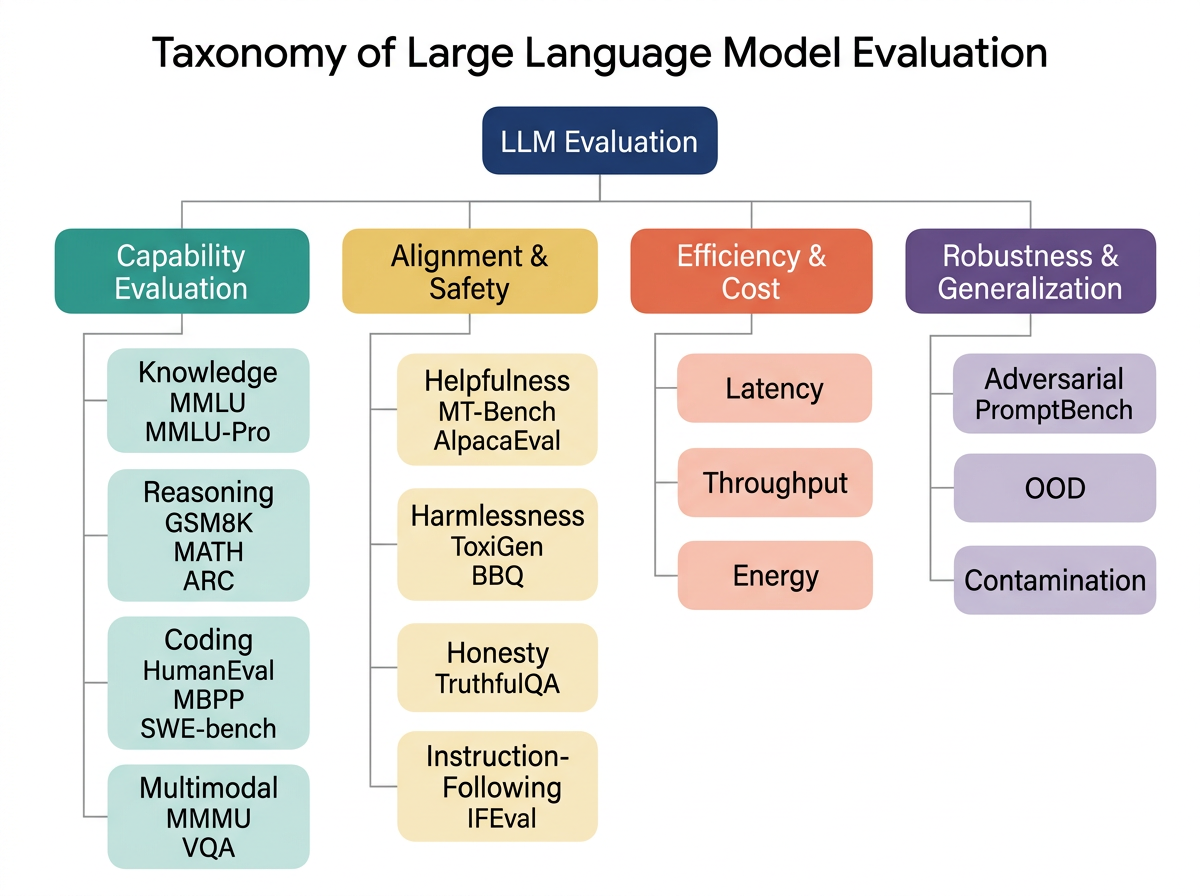
\includegraphics[width=\linewidth,keepaspectratio]{./figures/Evaluation-of-Large-Language-Models__fig2_taxonomy.png}}
\caption{Taxonomy of LLM Evaluation}\label{fig:fig2-taxonomy}\end{figure}

\subsection{Capability-Centric Axis: Knowledge, Reasoning, Code, Dialogue, Safety}\label{capability-centric-axis-knowledge-reasoning-code-dialogue-safety}

This subsection enumerates the six capability clusters and their canonical benchmarks. The capability axis groups benchmarks by what cognitive or behavioural property of the model they probe. Six clusters dominate the contemporary literature.

The \textbf{knowledge cluster} measures factual recall and reading comprehension. Massive Multitask Language Understanding (MMLU) \cite{hendrycks2021measuringmassivemu} is the canonical academic test with 15,908 four-way multiple-choice questions across 57 subjects organised into four super-categories: humanities, STEM, social sciences, and ``other'' (including law and medicine). TriviaQA \cite{joshi2017triviaqaalargescal} supplies 650k question-answer-evidence triples with closed-book and open-book splits. Natural Questions (NQ) \cite{kwiatkowski20192019} provides 307k real Google search queries paired with Wikipedia answers; the closed-book NQ score for GPT-3 175B is 14.6\%, while RAG-augmented LLaMA-2 reaches 38.4\% \cite{lewis20202020}. The wider MMLU family adds MMLU-Pro \cite{wang20242024}, which expands to 12,032 questions with ten options and harder distractors (GPT-4o 72.6\%, Claude 3 Opus 68.5\%), and MMLU-CF \cite{zhao20242024}, which removes likely-contaminated items. Chinese-language counterparts include C-Eval (13,948 questions across 52 subjects with four difficulty levels) \cite{huang20232023} and CMMLU (11,528 questions across 67 disciplines) \cite{li20242024}, while AGIEval {[}Zhong et al., 2023{]} aggregates 20 standardized human exams including the Chinese Gaokao, the SAT, and the Law School Admission Test.

The \textbf{reasoning cluster} stresses multi-step logical, mathematical, and commonsense inference. Grade School Math 8K (GSM8K) \cite{cobbe20212021} contains 7,473 training and 1,319 test arithmetic word problems; chain-of-thought prompting \cite{wei2022emergentabilitieso} raised accuracy from 17\% to 56.9\% for a 540B PaLM model and self-consistency raised it further to 74.8\%. The MATH benchmark \cite{hendrycks2021measuringmassivemu} supplies 12,500 competition-level problems graded across five difficulty levels with categories Algebra, Counting \& Probability, Geometry, Intermediate Algebra, Number Theory, Prealgebra, and Precalculus. BIG-Bench (Beyond the Imitation Game) \cite{srivastava20222022} gathers 204 diverse tasks contributed by 442 authors across 132 institutions; its 23-task BIG-Bench Hard (BBH) subset \cite{suzgun2022challengingbigbenc} singles out tasks where pre-2022 models trail humans by a wide margin. BBH includes \(causal_j\)udgement, \(date_u\)nderstanding, \(disambiguation_q\)a, hyperbaton, \(logical_d\)eduction, \(movie_r\)ecommendation, navigate, \(object_c\)ounting, \(penguins_i\)n\_a\_table, \(reasoning_a\)bout\_colored\_objects, \(ruin_n\)ames, \(salient_t\)ranslation\_error\_detection, snarks, \(sports_u\)nderstanding, \(temporal_s\)equences, and \(tracking_s\)huffled\_objects (3, 5, and 7 objects), among others. BIG-Bench Extra Hard \cite{kazemi20252025} further raises the bar for frontier models. Graduate-level reasoning is targeted by GPQA \cite{rein2024gpqaagraduatelevel} with 448 multiple-choice questions in biology, physics, and chemistry written by domain PhDs; the GPQA-Diamond subset (198 items) is the hardest tier with non-expert humans scoring 34\% and frontier models 50-71\%. HellaSwag \cite{zellers2019hellaswagcanamachi} (70k items) targets commonsense completion, ARC \cite{clark2018thinkyouhavesolved} supplies 7,787 grade-school science items split into Easy (5,197) and Challenge (2,590), and WinoGrande \cite{sakaguchi2020winograndeanadvers} provides 44k Winograd-schema items.

The \textbf{code cluster} evaluates program synthesis and software engineering. HumanEval \cite{chen20212021} is a hand-written set of 164 Python problems with hidden unit tests; pass@1 scores range from Codex 28.8\% to GPT-4 67-88\% to Claude 3.5 Sonnet 92\%. MBPP \cite{austin20212021} provides 974 mostly basic Python problems crowdsourced via internal annotators. MultiPL-E \cite{cassano20232023} translates HumanEval and MBPP into 18 languages including Java, JavaScript, C++, Rust, Go, Ruby, PHP, and Lua. Concrete repository-level evaluation begins with SWE-bench \cite{jimenez20242024}, 2,294 GitHub issues drawn from 12 popular Python projects; SWE-bench Verified is a 500-issue human-curated subset and SWE-Bench-Live extends to fresh issues. CoderEval \cite{yu20242024} examines pragmatic generation with 230 Python and 230 Java tasks with hidden test cases that include realistic dependencies. LiveCodeBench supplies a rolling stream of competitive-programming items time-stamped to combat contamination.

The \textbf{dialogue cluster} covers multi-turn instruction-following and chat quality. MT-Bench \cite{zheng20232023} presents 80 multi-turn questions across writing, roleplay, extraction, reasoning, math, coding, STEM, and humanities. AlpacaEval and AlpacaEval 2 \cite{taori2023stanfordalpacaanin} use 805 instruction prompts and report length-controlled win-rate against a reference model. Arena-Hard \cite{li20242024} curates 500 challenging prompts from real Chatbot Arena queries with 0.98 correlation to human Elo. Chatbot Arena \cite{chiang20242024} crowdsources pairwise battles in the wild, accumulating more than two million votes by 2024. MT-Bench-101 \cite{bai20242024} expands MT-Bench with 4,208 multi-turn samples across 13 abilities.

The \textbf{safety and alignment cluster} measures truthfulness, bias, toxicity, and jailbreak resistance. TruthfulQA \cite{lin2022truthfulqameasurin} presents 817 questions across 38 categories testing imitative falsehoods. BBQ \cite{parrish20222022} supplies 58,492 questions probing 11 social-bias categories. StereoSet \cite{nadeem2021stereosetmeasuring} measures stereotypical bias across gender, race, profession, and religion. RealToxicityPrompts contains 100k prompts triggering varying degrees of toxic continuation. AdvBench (520 harmful instructions) and HarmBench (510 harmful behaviours across seven categories) underpin red-teaming. GPTFUZZER \cite{yu2023gptfuzzerredteamin} auto-generates jailbreak prompts.

The \textbf{multimodal cluster}, while peripheral to text-only LLM evaluation, has become important for vision-language models. MME \cite{fu20232023} aggregates 14 sub-tasks across perception and cognition; LVLM-eHub \cite{xu20232023} benchmarks vision-language models across 47 tasks; the Yin et al.~survey on MLLMs \cite{yin20232023} catalogues this rapidly growing space.

\subsection{Methodology Axis: Static Splits, Live Arenas, Dynamic Generation}\label{methodology-axis-static-splits-live-arenas-dynamic-generation}

This subsection partitions benchmarks by curation methodology and lists the four canonical regimes. Representative methods include: static splits MMLU (2020), GSM8K (2021), HumanEval (2021), BIG-Bench (2022), and ARC (2018); live arenas Chatbot Arena (2023, 10M+ battles by 2026), Arena-Hard (2024, 0.98 Spearman with Elo), SWE-Bench-Live (2025); dynamic-generation systems Dynamic-KGQA (2025, knowledge-graph QA), DynaCode (2025, controlled cyclomatic complexity), and Jailbreak Distillation (2025, renewable safety probes); and adversarial-robustness suites PromptBench (2023, 10 attack types), PPTC-R (2024, PowerPoint robustness), and Atoxia (2024, targeted toxic triggers).

The methodology axis distinguishes how the evaluation set is curated and updated. \textbf{Static splits} (MMLU, GSM8K, HumanEval, BIG-Bench, ARC, HellaSwag) freeze a question set, publish it openly, and accept that contamination will increase over time. Static splits offer reproducibility but risk benchmark obsolescence; the AI Benchmark Half-Life paper \cite{white20242024} estimates that under uncontrolled re-training, the validity of a public benchmark decays exponentially with a half-life of about 12-18 months for popular suites.

\textbf{Live arenas} update continuously. Chatbot Arena \cite{chiang20242024} solicits new pairwise battles every minute; Arena-Hard \cite{li20242024} periodically re-derives a 500-prompt set from recent activity; BenchBuilder automates curation. SWE-Bench-Live extends SWE-bench with fresh GitHub issues post-dating the model's training cutoff. Live arenas combat contamination at the cost of reproducibility --- running an open-weights model on Arena requires an API endpoint and human voters.

\textbf{Dynamic generation} synthesises new test items on demand. Dynamic-KGQA \cite{dammu2025dynamickgqaascalab} generates question-answer pairs from a knowledge graph; DynaCode \cite{hu20252025} generates code problems with controlled complexity; Jailbreak Distillation \cite{zhang20252025} generates renewable safety probes. Dynamic generation interpolates between static and live: items can be regenerated to defeat memorisation, and the generation process is reproducible if the seed and template are released.

A fourth methodology, \textbf{adversarial robustness evaluation}, combines static probes with adversarial perturbations. PromptBench supplies adversarial prompt rewrites across 10 attack types (character, word, sentence, semantic). PPTC-R \cite{zhang20242024} evaluates robustness of PowerPoint task completion under prompt perturbations. The Atoxia framework \cite{du20242024} generates targeted toxic-output triggers for red-teaming. Robustness scores are typically reported as a delta from clean accuracy.

\subsection{Domain Axis: General-Purpose, Medical, Legal, Financial, Multilingual}\label{domain-axis-general-purpose-medical-legal-financial-multilingual}

This subsection cross-cuts the previous two axes by application domain.

The domain axis cuts across the capability and methodology axes. \textbf{General-purpose} suites --- HELM, BIG-Bench, OpenLLM Leaderboard --- span no single domain. \textbf{Medical} evaluation centres on MedQA (US Medical Licensing Exam--style, 12,723 questions), PubMedQA (1k expert-annotated yes/no items), MedMCQA (194k items), and MMLU's clinical knowledge subjects. The Med-PaLM line \cite{singhal20232023,singhal20252025} reports Med-PaLM's 67.6\% MedQA score and Med-PaLM 2's 86.5\%, with GPT-4 reaching 86.7\% on Step 2/3 USMLE \cite{nori2023capabilitiesofgpt4}. AgentClinic \cite{schmidgall20262026} evaluates LLM agents in interactive clinical scenarios with 24 differential diagnosis tasks. \textbf{Legal} evaluation includes LegalBench (162 tasks), CaseHOLD, CUAD, and bar-exam style probes. \textbf{Financial} evaluation includes FinGPT \cite{wang20232023}, FinBen, FinanceBench, and the symbolic chain-of-thought benchmark FinChain \cite{xie20252025}. \textbf{Multilingual} evaluation aggregates XNLI \cite{conneau20182018} (15 languages), MEGA \cite{ahuja20232023} (16 languages, 22 datasets), MGSM {[}Shi et al., 2022{]} (250 GSM8K items translated into 10 languages), BIG-Bench Hard multilingual variants, BnMMLU (Bengali) \cite{joy2025bnmmlumeasuringmas}, and Mobile-MMLU \cite{bsharat20252025} (16,186 mobile-style queries).

A practical implication of the multi-axis view is that comparing two models requires specifying a target \emph{cell} in the (capability × methodology × domain) grid, not just citing a single number. A model with state-of-the-art MMLU (knowledge × static × general) may underperform a competitor on Chatbot Arena Elo (dialogue × live × general) and on MedQA (knowledge × static × medical). The HELM framework \cite{liang20222022} explicitly reports across many cells; the Open LLM Leaderboard reports a six-benchmark composite (ARC, HellaSwag, MMLU, TruthfulQA, WinoGrande, GSM8K) that covers four capability slots but only static-general methodology.

The table below maps representative benchmarks to taxonomy coordinates.

\begin{table*}[t]
\centering
\caption{Domain Axis: General-Purpose, Medical, Legal, Financial, Multilingual: comparative summary.}
\label{tab:domain-axis-general-purpose-medical-legal-financial-multilin}
\begin{tabular}{>{\raggedright\arraybackslash}p{0.1667\linewidth}
  >{\raggedright\arraybackslash}p{0.1538\linewidth}
  >{\raggedright\arraybackslash}p{0.1795\linewidth}
  >{\raggedright\arraybackslash}p{0.1538\linewidth}
  >{\raggedright\arraybackslash}p{0.1538\linewidth}
  >{\raggedright\arraybackslash}p{0.1923\linewidth}}
\toprule
Benchmark & Capability & Methodology & Domain & Items & Key Citation \\
\midrule
MMLU & Knowledge & Static & General & 15,908 & Hendrycks 2021 \\
MMLU-Pro & Knowledge & Static (CF) & General & 12,032 & Wang 2024 \\
GSM8K & Reasoning & Static & General & 8,792 & Cobbe 2021 \\
MATH & Reasoning & Static & General & 12,500 & Hendrycks 2021 \\
BIG-Bench & Multi & Static & General & 204 tasks & Srivastava 2022 \\
BBH & Reasoning & Static & General & 23 tasks & Suzgun 2022 \\
GPQA-Diamond & Reasoning & Static & Science & 198 & Rein 2024 \\
HumanEval & Code & Static & General & 164 & Chen 2021 \\
MBPP & Code & Static & General & 974 & Austin 2021 \\
MultiPL-E & Code & Static & General & 164×18 langs & Cassano 2023 \\
SWE-bench & Code & Static + Live & General & 2,294 & Jimenez 2024 \\
MT-Bench & Dialogue & Static (judge) & General & 80 & Zheng 2023 \\
Chatbot Arena & Dialogue & Live & General & 2M+ votes & Chiang 2024 \\
Arena-Hard & Dialogue & Static (judge) & General & 500 & Li 2024 \\
TruthfulQA & Safety & Static & General & 817 & Lin 2022 \\
BBQ & Safety/Bias & Static & General & 58,492 & Parrish 2022 \\
HarmBench & Safety & Static & General & 510 & Mazeika 2024 \\
RULER & Long-context & Synthetic & General & 13 sub-tasks & Hsieh 2024 \\
GAIA & Agent & Static & General & 466 & Mialon 2024 \\
AgentBench & Agent & Static & General & 8 envs & Liu 2023 \\
MedQA & Knowledge & Static & Medical & 12,723 & Jin 2021 \\
C-Eval & Knowledge & Static & Chinese & 13,948 & Huang 2023 \\
CMMLU & Knowledge & Static & Chinese & 11,528 & Li 2024 \\
MEGA & Multi & Static & Multilingual & 22 datasets & Ahuja 2023 \\
MGSM & Reasoning & Static & Multilingual & 250×10 & Shi 2022 \\
\end{tabular}
\end{table*}

This taxonomy is intentionally disjoint at top level: a benchmark belongs to exactly one capability primary cluster, although it may have secondary memberships (e.g., MultiPL-E is primarily code but also multilingual). Throughout the rest of the survey we cite a benchmark with its taxonomy coordinates implicit; when a discussion turns on the methodology axis (e.g., live arenas in Section 6.3) we make the coordinate explicit. The taxonomy will also organise our discussion of failure modes in Section 11, where contamination, prompt sensitivity, and saturation each affect different cells of the grid.

\section{Historical Trajectory: From GLUE to Humanity's Last Exam}\label{historical-trajectory-from-glue-to-humanitys-last-exam}

Building on the taxonomy of Section 3, this section retraces the chronological trajectory along which the cells of that grid were populated. This section reviews the field's evolution in three eras, organised as the pre-transformer era (Section 4.1), the few-shot pivot (Section 4.2), and the post-ChatGPT reorientation (Section 4.3).

The history of LLM evaluation traces a quarter-century arc that runs from string-similarity metrics for machine translation to multi-million-dollar live arenas for chatbots. Three eras are most informative: the pre-transformer era (2002-2018), the few-shot pivot of GPT-3 and the early MMLU/BIG-Bench wave (2019-2022), and the post-ChatGPT period of holistic, live, and agentic evaluation (2023-2026). The narrative below establishes the sequence of seminal benchmarks, the metric inventions that drove each transition, and the model releases that crystallised the corresponding evaluation regime.

\subsection{Pre-Transformer Metrics and the GLUE/SuperGLUE Era (2002-2019)}\label{pre-transformer-metrics-and-the-gluesuperglue-era-2002-2019}

This subsection traces the metric and benchmark stack that preceded the GPT-3 few-shot pivot. Representative artefacts of this era include: BLEU (2002, n-gram MT precision), ROUGE-1/2/L (2004, summarisation recall), METEOR (2005, WordNet-aware matching), TER (2006, translation edit rate), chrF (2015, character n-gram F1), SQuAD (2016, 107k QA triples), GLUE (2018, 9 sentence-pair tasks), SuperGLUE (2019, 8 harder tasks), BERTScore (2020, RoBERTa-large embeddings), MoverScore (2019, EMD over token alignments), Sentence Mover's Similarity (2019), BLEURT (2020, learned regressor), and CLIPScore (2021, image-caption reference-free).

The first widely adopted automatic metric for natural-language generation was the Bilingual Evaluation Understudy (BLEU) score introduced by Papineni et al.~at IBM in 2002 \cite{papineni2002bleuamethodforauto}. BLEU computes the geometric mean of modified \(n\)-gram precisions for \(n \in \{1, 2, 3, 4\}\) between candidate translations and human references, multiplied by a brevity penalty. Despite the well-documented gap between BLEU and human judgement, BLEU has been used to score every major machine-translation system since the early IBM/SRI work and is reported in the LLaMA technical paper \cite{touvron20232023} for WMT-style translation evaluation. ROUGE (Recall-Oriented Understudy for Gisting Evaluation) \cite{lin2004rougeapackageforau} introduced ROUGE-N (n-gram recall), ROUGE-L (longest common subsequence), and ROUGE-W (weighted LCS) for summarisation. METEOR (2005), TER (2006), and chrF (2015) refined the family.

Reading-comprehension evaluation was reshaped by the Stanford Question Answering Dataset (SQuAD) \cite{rajpurkar2016squad100000questio}, which contained 107,785 question-answer-passage triples and used token-level F1 plus exact-match. SQuAD 2.0 added 53,775 unanswerable adversarial questions. Beyond machine-translation and reading-comprehension, the General Language Understanding Evaluation (GLUE) benchmark \cite{wang2018glueamultitaskbenc} aggregated nine sentence-pair tasks (CoLA, SST-2, MRPC, STS-B, QQP, MNLI, QNLI, RTE, WNLI). Within months of its release, BERT-large \cite{devlin2019bertpretrainingofd} surpassed previous state-of-the-art on every GLUE task, prompting the SuperGLUE benchmark \cite{wang2019superglueastickier} with eight harder tasks (BoolQ, CB, COPA, MultiRC, ReCoRD, RTE, WiC, WSC). Both GLUE and SuperGLUE saturated within two years of release, anticipating a recurring pattern in LLM evaluation.

In parallel, embedding-based generation metrics emerged. BERTScore \cite{zhang2020bertscoreevaluatin} used contextual RoBERTa-large embeddings (default reference layer 17) to compute token-level cosine similarity between candidate and reference; on the WMT-19 metrics task, BERTScore correlated with human judgement at Spearman 0.30-0.45, exceeding BLEU by 0.10. MoverScore (2019) extended BERTScore with Earth-Mover distance over soft alignments; CLIPScore (2021) \cite{hessel20212021} adapted the idea to image captioning. The Sentence Mover's Similarity metric (2019) and BLEURT (2020) trained learned regressors on human-judgement data to push correlations further.

The end of this era was marked by Brown et al.'s GPT-3 paper \cite{brown20202020}, which demonstrated few-shot generalisation across 24 tasks at the 175-billion-parameter scale. Few-shot evaluation, where \(k\) exemplars are concatenated to the test input, replaced fine-tune-and-evaluate as the standard release protocol for autoregressive LLMs. By the close of 2020, the field had a coherent metric stack (BLEU, ROUGE, BERTScore, EM, F1) and a coherent benchmark stack (GLUE, SuperGLUE, SQuAD, TriviaQA, NQ), but no comprehensive coverage of the multi-task generalisation that GPT-3 had begun to exhibit.

\subsection{The Few-Shot Pivot and MMLU/BIG-Bench Wave (2020-2022)}\label{the-few-shot-pivot-and-mmlubig-bench-wave-2020-2022}

This subsection covers the multi-task suites that emerged once GPT-3's few-shot generalisation made breadth a first-class evaluation criterion. Representative artefacts include: GPT-3 (2020, 175B parameters, 24-task few-shot suite), MMLU (2020, 15,908 items, 57 subjects), HumanEval (2021, 164 Python problems), GSM8K (2021, 7,473 train + 1,319 test items), MATH (2021, 12,500 competition problems), TruthfulQA (2022, 817 imitative-falsehood items), HellaSwag (2019, 70k commonsense items), WinoGrande (2020, 44k Winograd items), ARC (2018, 7,787 grade-school items), BIG-Bench (2022, 204 tasks, 442 contributors), BBH (2022, 23 hard tasks), HELM v1 (2022, 16 scenarios with 7 metrics), Chain-of-Thought prompting \citep{wei2022emergentabilitieso}, Self-Consistency (Wang 2023, 40-sample majority vote), Zero-shot CoT (Kojima 2022, ``Let's think step by step''), and PAL (Gao 2022, Python interpreter offload).

The years 2020-2022 saw the construction of large multi-task evaluation suites that aimed to match the breadth of GPT-3's emerging capabilities. Hendrycks et al.~introduced the Massive Multitask Language Understanding (MMLU) benchmark \cite{hendrycks2021measuringmassivemu} in late 2020 with 15,908 four-way multiple-choice items spread across 57 academic subjects. MMLU was specifically designed for in-context evaluation: a 5-shot protocol drew exemplars from a development split and asked the model to predict letter A-D. GPT-3 175B scored 43.9\% (random baseline 25\%); UnifiedQA, BERT-Large, and RoBERTa-base hovered between 28\% and 35\%. Within four years MMLU rose to 90.0\% with Gemini Ultra {[}Gemini Team, 2023{]}, 88.7\% with GPT-4o, 86.8\% with Claude 3 Opus, and 90.8\% with DeepSeek-R1 {[}DeepSeek-AI, 2025{]}, illustrating the saturation arc.

Hendrycks et al.~simultaneously released MATH \cite{hendrycks2021measuringmassivemu}, the first large-scale competition-mathematics benchmark with 12,500 problems graded across five difficulty levels and seven subjects (Algebra, Counting \& Probability, Geometry, Intermediate Algebra, Number Theory, Prealgebra, Precalculus). At the same Datasets \& Benchmarks track, OpenAI released Evaluating Large Language Models Trained on Code with the HumanEval benchmark \cite{chen20212021}, 164 hand-written Python problems with hidden unit tests. Cobbe et al.~\cite{cobbe20212021} introduced GSM8K with 7,473 train and 1,319 test grade-school arithmetic word problems. TruthfulQA \cite{lin2022truthfulqameasurin} emerged with 817 questions across 38 categories testing imitative falsehoods, with GPT-3 175B answering only 21\% truthfully on the multiple-choice format and 58\% imitative-false on the open-ended format.

The most ambitious single artefact of this era was BIG-Bench (Beyond the Imitation Game) \cite{srivastava20222022}, a community-built benchmark with 204 tasks contributed by 442 authors at 132 institutions. BIG-Bench standardised tasks as JSON files with input-target pairs and a metric specification, allowing automatic evaluation across heterogeneous capabilities. PaLM-540B reached an average normalized score of 0.55 on BIG-Bench. The BIG-Bench Hard (BBH) subset \cite{suzgun2022challengingbigbenc} selected the 23 tasks where pre-2022 models trailed the average human worker; chain-of-thought prompting raised average BBH accuracy from 50\% to 67\%.

A key methodological innovation of this era was \emph{chain-of-thought (CoT) prompting} \cite{wei2022emergentabilitieso}, which inserts intermediate reasoning steps in few-shot exemplars. CoT raised PaLM-540B's GSM8K accuracy from 17\% to 56.9\%, and self-consistency (40 sampled chains, majority vote) \cite{wang20232023} further raised it to 74.8\%. Zero-shot CoT via the trigger ``Let's think step by step'' \cite{kojima2022largelanguagemodel} gave smaller but still meaningful gains. Program-aided language models (PAL) {[}Gao et al., 2022{]} outsourced arithmetic to a Python interpreter, reaching 72\% on GSM8K with Codex.

The era ended with two complementary releases. Liang et al.'s Holistic Evaluation of Language Models (HELM) \cite{liang20222022} consolidated 16 scenarios under seven metrics --- accuracy, calibration, robustness, fairness, bias, toxicity, efficiency --- and ran 30+ models through the full panel. The HELM artefact remains the most extensive single evaluation effort and continues to expand through 2024-2025. In late 2022, OpenAI released ChatGPT, which forced a methodological reckoning: free-form chat could not be scored by BLEU, EM, or pass@k. The community responded with judge-based protocols.

\subsection{Post-ChatGPT Reorientation Toward Holistic, Live, and Agentic Evaluation (2023-2026)}\label{post-chatgpt-reorientation-toward-holistic-live-and-agentic-evaluation-2023-2026}

This subsection covers the three intertwined shifts that defined the post-ChatGPT evaluation reorientation: judge-based scoring, live arenas, and agentic benchmarks. Representative artefacts include: MT-Bench (2023, 80 multi-turn questions, GPT-4 judge), Chatbot Arena (2023, 10M+ pairwise battles by 2026), AlpacaEval (2023, 805 instructions), AlpacaEval 2 LC (2024, length-controlled win-rate), G-Eval (2023, GPT-4 rubric judge), Arena-Hard (2024, 500 BenchBuilder prompts, 0.98 Spearman with Elo), MMLU-Pro (2024, 12,032 items, 10 options), MMLU-CF (2024, 8,000 leakage-screened items), GPQA-Diamond (2024, 198 graduate-science items), Humanity's Last Exam (2025, 3,000+ frontier items), GAIA (2024, 466 generalist-agent questions), AgentBench (2023, 8 environments), MLE-bench (2024, 75 Kaggle competitions), SWE-bench (2024, 2,294 GitHub issues), SWE-bench Verified (2024, 500 human-curated issues), SWE-Bench-Live (2025), RULER (2024, 13 long-context sub-tasks up to 128k), GSM1k (2024, 1,250 contamination probes), and DeepSeek-R1 (2025, reasoning-trained 90.8\% MMLU).

The post-ChatGPT period is characterised by three intertwined shifts: the rise of LLM-as-a-Judge for open-ended generation, the emergence of live and contamination-aware evaluation, and the incorporation of agentic and tool-using tasks into the evaluation canon.

Zheng et al.'s MT-Bench paper \cite{zheng20232023} introduced both the 80-question multi-turn chat benchmark and the LMSYS Chatbot Arena, where pairwise battles between anonymised models accumulated 2 million votes by 2024 \cite{chiang20242024}. The MT-Bench protocol asks GPT-4 to score two responses (A and B) against a rubric --- helpfulness, correctness, coherence, safety, conciseness --- with position swapping to control for order bias. Agreement with human preferences reached 80-85\%. AlpacaEval \cite{dubois20242024} simplified the protocol to win-rate against text-davinci-003. G-Eval \cite{liu2023gevalnlgevaluation} systematised LLM-as-Judge for summarisation and dialogue, producing Spearman correlations of 0.40-0.55 with human ratings. By 2024, Arena-Hard \cite{li20242024} curated 500 hard prompts and reported 0.98 Spearman correlation with human Elo, surpassing MMLU's 0.66 and MT-Bench's 0.95.

Sparks of Artificial General Intelligence \cite{bubeck20232023} examined GPT-4 across diverse tasks; the GPT-4 Technical Report {[}OpenAI, 2023{]} provided systematic numerical anchors: Uniform Bar Exam 90th-percentile, USMLE 86.7\%, MMLU 86.4\%, HumanEval 67\%, GSM8K 92\%. Anthropic's Claude family, Google DeepMind's Gemini line {[}Gemini Team, 2023; Gemini Team, 2024{]}, Meta's LLaMA-2/3 \cite{touvron20232023}, Mistral, and DeepSeek's V2/V3/R1 {[}DeepSeek-AI, 2025{]} each released technical reports following a roughly identical evaluation template --- a model card with MMLU, GSM8K, MATH, HumanEval, MBPP, BBH, ARC, HellaSwag, WinoGrande, GPQA, DROP, and SuperGLUE-style scores.

The contamination problem became central. Zhang et al.~\cite{zhang20242024} introduced GSM1k, a 1,250-problem set written from scratch matching GSM8K's distribution; some open-weights LLMs dropped 8-13 percentage points from GSM8K to GSM1k, signalling memorisation. The CONDA workshop in 2024 \cite{sainz20242024} consolidated contamination-detection methods (n-gram overlap, Min-K\%-Prob, perplexity gap, MIA) and reported 60+ submissions. The taxonomy of Palavalli et al.~\cite{palavalli2024ataxonomyfordataco} distinguished input contamination, label contamination, and order contamination. Contamination-aware benchmarks responded: MMLU-CF \cite{zhao20242024} removed likely-leaked items, MMLU-Pro \cite{wang20242024} tightened distractors and increased options to ten, and live arenas became preferred for instruction-following measurement.

Long-context evaluation emerged once Gemini 1.5 Pro's 1-2M-token context {[}Gemini Team, 2024{]} and Anthropic Claude 3 Opus's 200k context made the question pressing. Kamradt's Needle In A Haystack (NIAH) test \cite{kamradt2023needleinahaystackp} became viral in 2023, but Hsieh et al.'s RULER \cite{hsieh20242024} showed that NIAH's single-hop retrieval is insufficient and introduced 13 sub-tasks across retrieval, multi-hop tracing, aggregation, and QA up to 128k tokens. Llama-3-70B-128k retains 88\% RULER accuracy at 32k context but drops to 45\% at 128k. LongBench, BABILong, ZeroSCROLLS, and InfiniteBench complement RULER.

Agentic evaluation matured. SWE-bench \cite{jimenez20242024} shocked the community by showing that even GPT-4 with retrieval-augmented generation solves under 2\% of real GitHub issues; by 2025, SWE-Bench Verified leaderboards saw Claude 3.5 Sonnet plus the SWE-agent scaffold \cite{yang20242024} reaching 50\%. AgentBench \cite{liu2023gevalnlgevaluation} aggregated eight environments (operating system, database, knowledge graph, lateral thinking, web shopping, web browsing, household, gaming). GAIA \cite{mialon2024gaiaabenchmarkforg} introduced 466 questions across three difficulty levels designed to resist crawl-based contamination; in early 2024 GPT-4 with plugins scored 14.6\% versus humans' 92\%. MLE-bench \cite{chan20242024} examined ML-engineering capability via 75 Kaggle competitions. Yehudai et al.'s \cite{yehudai20252025} and Mohammadi et al.'s \cite{mohammadi20252025} surveys consolidated this rapidly growing agent-evaluation literature.

The most recent benchmarks aim at the frontier: GPQA-Diamond's 198 graduate-level questions \cite{rein2024gpqaagraduatelevel}, FrontierMath's research-level mathematics, and Humanity's Last Exam \cite{phan20252025} with 3,000+ questions across humanities, sciences, and mathematics where GPT-4o scores 5.7\% and o1 18\%. BIG-Bench Extra Hard \cite{kazemi20252025} extends BBH to nine harder reasoning skills.

The table below condenses the historical trajectory.

\begin{table*}[t]
\centering
\caption{Post-ChatGPT Reorientation Toward Holistic, Live, and Agentic Evaluation (2023-2026): comparative summary.}
\label{tab:post-chatgpt-reorientation-toward-holistic-live-and-agentic-}
\begin{tabular}{>{\raggedright\arraybackslash}p{0.0185\linewidth}
  >{\raggedright\arraybackslash}p{0.7130\linewidth}
  >{\raggedright\arraybackslash}p{0.2685\linewidth}}
\toprule
Year & Milestone & Key Anchor \\
\midrule
2002 & BLEU {[}Papineni{]} & \(n\)-gram MT metric \\
2004 & ROUGE {[}Lin{]} & Summarisation metric \\
2016 & SQuAD {[}Rajpurkar{]} & 107k QA pairs, EM/F1 \\
2018 & GLUE {[}Wang{]} & 9 sentence-pair tasks \\
2019 & SuperGLUE {[}Wang{]} & 8 harder tasks \\
2020 & BERTScore {[}Zhang{]}, GPT-3 {[}Brown{]} & Embedding-metric, 175B few-shot \\
2021 & MMLU {[}Hendrycks{]}, MATH, HumanEval {[}Chen{]}, GSM8K {[}Cobbe{]}, TruthfulQA {[}Lin{]} & 57 subjects, 12.5k math, 164 code, 8.5k math, 817 truthful \\
2022 & BIG-Bench {[}Srivastava{]}, BBH {[}Suzgun{]}, CoT {[}Wei{]}, Self-Cons. {[}Wang{]}, HELM {[}Liang{]}, InstructGPT {[}Ouyang{]} & 204 tasks, 23 subset, +11pp BBH avg \\
2023 & GPT-4 {[}OpenAI{]}, Sparks {[}Bubeck{]}, MT-Bench {[}Zheng{]}, Chatbot Arena, AlpacaEval, AgentBench {[}Liu{]}, SWE-bench {[}Jimenez{]}, LLaMA {[}Touvron{]}, Gemini {[}Gemini Team{]} & 86.4\% MMLU, 80q MT-Bench, 2294 issues \\
2024 & MMLU-Pro {[}Wang{]}, MMLU-CF, RULER {[}Hsieh{]}, Arena-Hard {[}Li{]}, GAIA {[}Mialon{]}, MLE-bench, Gemini 1.5, Claude 3, GSM1k {[}Zhang{]} & 12k items, 0.98 Spearman, 466 agent Q \\
2025 & DeepSeek-R1 {[}DeepSeek-AI{]}, BBEH {[}Kazemi{]}, GPQA, Humanity's Last Exam {[}Phan{]}, SWE-Bench Verified & 90.8\% MMLU, 198 GPQA-D, 18\% HLE for o1 \\
2026 & Live arenas, agent benchmarks dominant & Predicted: SWE-Bench-Live, Arena-Hard, FrontierMath \\
\end{tabular}
\end{table*}

Two long-running tensions structure this trajectory. The first is the \emph{coverage versus depth} tension: GLUE/SuperGLUE were narrow but deeply analysed; BIG-Bench was broad but uneven. HELM addressed this with a structured panel; modern leaderboards (Open LLM, HELM Capability) sample several axes at once. The second is the \emph{contamination versus reproducibility} tension: live arenas combat contamination but are unreproducible; static splits are reproducible but contaminate. Hybrid approaches (Arena-Hard derived from live data; SWE-Bench-Live with rolling cutoffs; MMLU-CF with leakage-screened items) attempt to bridge the two.

We close this section with an empirical observation: every major benchmark introduced before 2022 has saturated to within 5 percentage points of its ceiling by 2025, and benchmarks introduced in 2023-2024 are saturating in 12-18 months. The remainder of the survey will repeatedly grapple with the question of how to design an evaluation that does not saturate within a release cycle.

\section{Knowledge and Reasoning Benchmarks: MMLU, BIG-Bench, GSM8K, MATH, GPQA}\label{knowledge-and-reasoning-benchmarks-mmlu-big-bench-gsm8k-math-gpqa}

Whereas Section 4 traced the chronology of evaluation, this section drills into the knowledge-and-reasoning cluster that dominates technical releases. This section reviews four benchmark families: the MMLU family (Section 5.1), BIG-Bench and its hard variants (Section 5.2), mathematical-reasoning suites (Section 5.3), and frontier-knowledge tests (Section 5.4). Representative methods include: MMLU (Hendrycks 2020, 15,908 4-way MCQ across 57 subjects), MMLU-Pro (Wang 2024, 12,032 10-way harder items), MMLU-CF (Zhao 2024, 8,000 leakage-screened items), C-Eval (Huang 2023, 13,948 Chinese items), CMMLU (Li 2024, 11,528 Chinese items), AGIEval (Zhong 2023, 8,062 standardised exam items), BIG-Bench (Srivastava 2022, 204 tasks), BBH (Suzgun 2022, 23 hard tasks), BBEH (Kazemi 2025, 23 newly authored hard tasks), GSM8K (Cobbe 2021, 1,319 test items), GSM1k (Zhang 2024, 1,250 contamination probes), MATH (Hendrycks 2021, 12,500 competition problems), MATH-500 (subset for benchmarking), AIME 2024 (30 invitational items), FrontierMath (Glazer 2024, 300+ research-level items), GPQA-Diamond (Rein 2024, 198 graduate-science items), and Humanity's Last Exam (Phan 2025, 3,000+ frontier items).

Knowledge and reasoning benchmarks are the workhorse of LLM evaluation, accounting for the bulk of numbers reported in technical releases. We dedicate this section to a deep dive into the four most influential families: the MMLU family, the BIG-Bench family, the mathematical-reasoning family (GSM8K, MATH, AIME), and the frontier-knowledge family (GPQA, FrontierMath, Humanity's Last Exam). For each, we provide its size, structure, scoring protocol, and current numerical anchors across major frontier models.

\subsection{The MMLU Family: Original, Pro, CF, and Domain-Specific Variants}\label{the-mmlu-family-original-pro-cf-and-domain-specific-variants}

This subsection covers the MMLU family across original, contamination-resistant, and domain-specific variants.

The Massive Multitask Language Understanding (MMLU) benchmark was introduced by Hendrycks et al.~in 2020 and presented at ICLR 2021 \cite{hendrycks2021measuringmassivemu}. MMLU contains 15,908 four-way multiple-choice items across 57 subjects spanning four super-categories: humanities (e.g., professional law with 1,534 items, world religions, philosophy, U.S. foreign policy), STEM (college physics, college mathematics, abstract algebra, college chemistry, conceptual physics, computer security, electrical engineering, elementary mathematics, high school biology, high school chemistry, high school computer science, high school mathematics, high school physics, machine learning, college biology, college computer science), social sciences (econometrics, high school geography, high school government and politics, high school macroeconomics, high school microeconomics, high school psychology, human sexuality, professional psychology, public relations, security studies, sociology, US foreign policy, virology), and other (clinical knowledge, college medicine, global facts, human aging, international law, jurisprudence, marketing, medical genetics, miscellaneous, moral disputes, moral scenarios, nutrition, professional accounting, professional medicine, professional law). The official protocol is 5-shot with greedy decoding, with the answer extracted via either next-token log-probability comparison among A/B/C/D or by free generation. Per-subject scores are averaged uniformly. The randomly-guessing baseline is 25\%; UnifiedQA's score in 2020 was 48.9\%; GPT-3 175B reached 43.9\% in the original paper.

By the GPT-4 Technical Report {[}OpenAI, 2023{]}, MMLU 5-shot reached 86.4\%. Gemini Ultra reported 90.0\% {[}Gemini Team, 2023{]}; Claude 3 Opus reached 86.8\%; LLaMA-2-70B reached 68.9\%; LLaMA-3-70B reached 80.9\%; LLaMA-3.1-405B reached 87.3\%; Mistral Large 81.2\%; DeepSeek-V3 88.5\%; DeepSeek-R1 90.8\% {[}DeepSeek-AI, 2025{]}; GPT-4o 88.7\%; o1-preview 91.8\%. The saturation arc prompted MMLU-Pro \cite{wang20242024}, which expanded to 12,032 questions, increased the option count from four to ten, and selected harder items via GPT-4 verification. On MMLU-Pro, GPT-4o scored 72.6\%, Claude 3 Opus 68.5\%, GPT-4 71.0\%, LLaMA-3.1-405B 73.3\%, and DeepSeek-R1 84.0\%. Wang et al.~also introduced contamination filtering by comparing item embeddings against pre-training corpora.

MMLU-CF \cite{zhao20242024} is the contamination-free variant, removing items whose 13-gram overlap with the Pile, RedPajama, or C4 exceeds a threshold; the resulting 8,000-item set is intended as a leak-proof drop-in for MMLU. Domain-specific MMLU variants include the Chinese C-Eval \cite{huang20232023} with 13,948 items across 52 subjects and four difficulty levels, CMMLU \cite{li20242024} with 11,528 items across 67 disciplines, and ArabicMMLU, Mobile-MMLU \cite{bsharat20252025} (16,186 mobile-style queries), Video-MMLU \cite{song20252025} (lecture-comprehension multimodal), BnMMLU \cite{joy2025bnmmlumeasuringmas} (Bengali), and JMMLU (Japanese). The TCMI-F-6D benchmark \cite{teng20262026} adapts MMLU to Traditional Chinese Medicine Informatics.

A common practical concern with the MMLU family is the \emph{answer-extraction} variance. The lm-evaluation-harness uses next-token log-likelihood comparison \cite{biderman20242024}; the original paper used free generation followed by regex extraction; HELM uses a structured prompt with explicit ``Answer:'' cue. These three approaches can shift reported scores by 3-7 percentage points on identical models, an effect documented across the field.

\subsection{BIG-Bench, BBH, and BIG-Bench Extra Hard}\label{big-bench-bbh-and-big-bench-extra-hard}

This subsection covers the BIG-Bench family and its successive harder subsets.

BIG-Bench (Beyond the Imitation Game) \cite{srivastava20222022} is the broadest single LLM benchmark, with 204 tasks contributed by 442 authors at 132 institutions. Tasks are stored as JSON with input-target pairs and a metric specification (multiple-choice grade, exact match, BLEU, ROUGE, GPT-4-judge, etc.). Tasks span linguistic competence (anaphora resolution, syntactic well-formedness), reasoning (logical deduction, formal fallacies), social abilities (emoji semantics, persuasion), task-specific knowledge (programmatic translation, chess), and multilingual probes. BIG-Bench Lite is a 24-task curated subset (1,200 items total) for cheap evaluation. PaLM-540B reached an average normalized score of 0.55 on the full BIG-Bench, comparable to the human-rater average of 0.59.

BIG-Bench Hard (BBH) \cite{suzgun2022challengingbigbenc} selects 23 BIG-Bench tasks where pre-2022 LMs underperformed humans by a wide margin: \(boolean_e\)xpressions, \(causal_j\)udgement, \(date_u\)nderstanding, \(disambiguation_q\)a, \(dyck_l\)anguages, \(formal_f\)allacies, \(geometric_s\)hapes, hyperbaton, \(logical_d\)eduction (3, 5, 7 objects), \(movie_r\)ecommendation, \(multistep_a\)rithmetic\_two, navigate, \(object_c\)ounting, \(penguins_i\)n\_a\_table, \(reasoning_a\)bout\_colored\_objects, \(ruin_n\)ames, \(salient_t\)ranslation\_error\_detection, snarks, \(sports_u\)nderstanding, \(temporal_s\)equences, \(tracking_s\)huffled\_objects (3, 5, 7 objects), \(web_o\)f\_lies, and \(word_s\)orting. CoT prompting on Codex raised average BBH accuracy from 50.9\% (3-shot) to 73.9\% (3-shot CoT). Frontier models score 80-92\% on BBH today.

BIG-Bench Extra Hard (BBEH) \cite{kazemi20252025} extends BBH with 23 newly authored tasks across nine reasoning skills designed to challenge frontier reasoning models; many target compositional reasoning where simple pattern matching fails. Predictability of LM capabilities on BIG-Bench was studied by Ye et al.~\cite{ye2023howpredictablearel}, who showed that performance on a held-out task can be forecast within 4-7 points using cross-task transfer regression.

\subsection{Mathematical Reasoning: GSM8K, MATH, and Competition-Level Math}\label{mathematical-reasoning-gsm8k-math-and-competition-level-math}

This subsection traces the math benchmark stack from grade-school arithmetic to research-level mathematics.

Mathematical reasoning has become the most active sub-area of LLM evaluation, both because mathematics admits unambiguous grading and because reasoning-trained models (OpenAI o1, DeepSeek-R1, Gemini 2.0 Thinking) are explicitly optimised for it.

GSM8K \cite{cobbe20212021} contains 7,473 training and 1,319 test grade-school math problems with step-by-step solutions; problems require 2-8 steps of arithmetic. Single-shot accuracy went from GPT-3 175B's 17\% to PaLM-540B's 18\%; CoT raised PaLM to 56.9\% and self-consistency to 74.8\%. GPT-4 reaches 92\% with CoT; Claude 3 Opus 95\%; LLaMA-3-70B 80.6\%; LLaMA-3.1-405B 96.8\%; o1-preview 95\%; DeepSeek-R1 97.3\%. The accompanying GSM1k probe \cite{zhang20242024} tests 1,250 newly authored items in identical distribution; some open-weights models drop 8-13 points, indicating memorisation. MR-GSM8K {[}Zeng et al., 2023{]} extends GSM8K to meta-reasoning where the model must score solutions rather than produce them. Achieving \textgreater97\% on GSM8K \cite{zhong2024agievalahumancentr} documents the prompting techniques that close the last few points.

The MATH benchmark \cite{hendrycks2021measuringmassivemu} contains 12,500 competition problems graded across five difficulty levels (1=easy through 5=AIME-level) and seven subjects. GPT-4 reaches 35.7\% one-shot and 42.5\% with CoT; Minerva 540B 50.3\%; Toolformer 27\%; LLaMA-3-70B 50\%; LLaMA-3.1-405B 73.8\%; o1-preview 85.5\%; DeepSeek-R1 97.3\% on the MATH-500 subset. The AIME (American Invitational Mathematics Examination) and AMC subsets push the difficulty further: o1-preview reaches 56.7\% AIME; DeepSeek-R1 79.8\%. MGSM {[}Shi et al., 2022{]} translates 250 GSM8K items into 10 languages.

For competition-level mathematics, FrontierMath was introduced by Glazer et al.~(2024) with 300+ research-level problems written by professional mathematicians; even GPT-4o solved less than 2\% as of late 2024, while o1 solved roughly 13\%. InternLM-Math {[}Ying et al., 2024{]} released open weights specialised for verifiable mathematical reasoning. DiffCoT \cite{cao20262026} explores diffusion-style reasoning chains. The MATH-PT benchmark {[}Teixeira et al., 2026{]} adapts MATH to European and Brazilian Portuguese.

The dominant evaluation protocol on math benchmarks remains exact-match between extracted final answers; chain-of-thought scoring is increasingly augmented by \emph{process reward models} (PRMs) that score each reasoning step. The PRM800K dataset \citep{lightman20242024} provides 800k step-level human annotations and is used by OpenAI for o1's training and evaluation.

\subsection{Frontier Knowledge Tests: GPQA-Diamond and Humanity's Last Exam}\label{frontier-knowledge-tests-gpqa-diamond-and-humanitys-last-exam}

This subsection covers the benchmarks designed to retain headroom against the strongest 2025-2026 frontier models.

Frontier knowledge benchmarks are designed to remain hard for frontier models. GPQA (Graduate-level Google-Proof Q\&A) \cite{rein2024gpqaagraduatelevel} contains 448 multiple-choice questions in biology, physics, and chemistry written by domain PhDs, with extensive verification: each item is reviewed by at least two domain experts and rejected if non-experts can answer correctly with internet access. The GPQA-Diamond subset (198 items) is the hardest tier where non-expert human accuracy with 30 minutes of unrestricted Google access is 34\%, while expert humans reach 81\%. GPT-4 scores 39.4\%, Claude 3 Opus 60.1\%, GPT-4o 53.6\%, LLaMA-3.1-405B 51.1\%, o1-preview 78.3\%, DeepSeek-R1 71.5\%, and Claude 3.5 Sonnet 65\%.

Humanity's Last Exam (HLE) \cite{phan20252025} aggregates 3,000+ expert-written questions across mathematics, physics, biology, chemistry, computer science, history, philosophy, and the humanities, designed so that a Ph.D.~holder in the relevant field can answer but a non-expert cannot. GPT-4o scores 5.7\%, Claude 3.5 Sonnet 4.3\%, Gemini 1.5 Pro 5.0\%, o1 18\%, and DeepSeek-R1 14\%. HLE positions itself explicitly as a benchmark that should retain headroom for the next model generation.

AGIEval {[}Zhong et al., 2023{]} aggregates 20 standardized human exams (Chinese Gaokao, SAT, LSAT, the Chinese lawyer qualification, GMAT, the Chinese Civil Service Exam, AP courses, and more), with 8,062 multilingual items. SuperGLUE-Pro and BBH-Pro continue the trend of harder benchmarks. The Critical Review of Causal Reasoning Benchmarks \cite{yang20242024} finds that many causal benchmarks can be solved by domain-knowledge retrieval rather than genuine causal inference, prompting refinements such as the IIB benchmark.

The table below condenses key reasoning benchmark numbers across frontier models.

\begin{table*}[t]
\centering
\caption{Frontier Knowledge Tests: GPQA-Diamond and Humanity's Last Exam: comparative summary.}
\label{tab:frontier-knowledge-tests-gpqa-diamond-and-humanity-s-last-ex}
\begin{tabular}{>{\raggedright\arraybackslash}p{0.1477\linewidth}
  >{\raggedright\arraybackslash}p{0.1136\linewidth}
  >{\raggedright\arraybackslash}p{0.0568\linewidth}
  >{\raggedright\arraybackslash}p{0.1477\linewidth}
  >{\raggedright\arraybackslash}p{0.1364\linewidth}
  >{\raggedright\arraybackslash}p{0.1591\linewidth}
  >{\raggedright\arraybackslash}p{0.1250\linewidth}
  >{\raggedright\arraybackslash}p{0.1136\linewidth}}
\toprule
Benchmark & Items & GPT-4 & Claude 3 Opus & Gemini Ultra & LLaMA-3.1-405B & DeepSeek-R1 & o1-preview \\
\midrule
MMLU 5-shot & 15,908 & 86.4\% & 86.8\% & 90.0\% & 87.3\% & 90.8\% & 91.8\% \\
MMLU-Pro & 12,032 & 71.0\% & 68.5\% & --- & 73.3\% & 84.0\% & --- \\
BBH & 23 tasks & 86.7\% & 86.8\% & 83.6\% & 84.8\% & --- & --- \\
GSM8K & 1,319 test & 92.0\% & 95.0\% & 94.4\% & 96.8\% & 97.3\% & 95.0\% \\
MATH (5-shot) & 12,500 & 42.5\% & 60.1\% & 53.2\% & 73.8\% & 97.3\% & 85.5\% \\
AIME 2024 & 30 & --- & --- & --- & --- & 79.8\% & 56.7\% \\
GPQA-Diamond & 198 & 39.4\% & 60.1\% & --- & 51.1\% & 71.5\% & 78.3\% \\
HumanEval & 164 & 88.4\% & 84.9\% & 74.4\% & 89.0\% & 96.3\% & 92.4\% \\
HellaSwag & 10,003 & 95.3\% & 95.4\% & 87.8\% & 92.0\% & --- & --- \\
ARC-Challenge & 2,590 & 96.3\% & 96.4\% & --- & 96.1\% & --- & --- \\
WinoGrande & 1,267 & 87.5\% & 88.5\% & --- & 86.7\% & --- & --- \\
HLE (ours) & 3,000+ & --- & 4.3\% & --- & --- & 14\% & 18\% \\
\end{tabular}
\end{table*}

(Where a cell is dashed, the model report did not disclose the score under the official protocol.)

Several recurring themes emerge from the table. First, MMLU/HumanEval/HellaSwag/ARC are saturated in the sense that the gap between frontier model and human ceiling is now within 2-5 points; meaningful differentiation requires MMLU-Pro, GPQA-Diamond, AIME, and HLE. Second, reasoning-trained models (DeepSeek-R1, o1-preview) systematically outperform standard models on math and graduate-level science, often by 10-20 points, while underperforming or matching on knowledge-pure benchmarks (MMLU, HellaSwag). Third, the benchmark numbers reported in different model releases use different protocols (some include CoT, some only single-shot; some report best-of-N, some only greedy), so cross-source comparison must be done with care.

This section has provided locally answerable facts about MMLU's 57 subjects and 15,908 items, BIG-Bench's 204 tasks and 442 contributors, GSM8K's 1,319 test problems, MATH's 12,500 problems and five difficulty levels, GPQA-Diamond's 198 items, and Humanity's Last Exam's 3,000+ questions. The next section turns to the metrics and judging machinery used to score open-ended generations.

\section{Generation Quality Metrics and the Rise of LLM-as-a-Judge}\label{generation-quality-metrics-and-the-rise-of-llm-as-a-judge}

Whereas Section 5 covered closed-form knowledge and reasoning tests, this section turns to the open-ended generation regime where reference-based metrics break down. This section reviews the contemporary metric stack in three subsections: classical reference-based metrics (Section 6.1), the LLM-as-a-Judge paradigm (Section 6.2), and pairwise human preference via Chatbot Arena (Section 6.3). Representative methods include: BLEU \citep{papineni2002bleuamethodforauto}, ROUGE-L \citep{lin2004rougeapackageforau}, METEOR (Banerjee 2005), chrF (Popović 2015), BERTScore \citep{zhang2020bertscoreevaluatin}, MoverScore (Zhao 2019), BARTScore (Yuan 2021), BLEURT (Sellam 2020), CLIPScore \citep{hessel20212021}, G-Eval (Liu 2023, GPT-4 rubric judge), MT-Bench (Zheng 2023, 80 multi-turn questions), AlpacaEval 2 LC (Dubois 2024, 805 instructions), Arena-Hard (Li 2024, 500 BenchBuilder prompts, 0.98 Spearman), Prometheus (Kim 2024, open 13B judge), Prometheus 2 (2024, 7B/8x7B), JudgeLM (2023, open judge), PandaLM (2023, open judge), MD-Judge (2024), Chatbot Arena (Chiang 2024, 10M+ battles by 2026), and FActScore (Min 2023, atomic-fact verification).

The shift from closed-form classification to open-ended generation as the primary use case of LLMs has rendered classical reference-based metrics inadequate. Open-ended dialogue, summarisation, creative writing, and instruction following do not have a single gold answer; many fluent, factually correct responses exist for any given prompt. This section traces the metric stack that has emerged in response: reference-based (BLEU, ROUGE, METEOR, chrF, BERTScore, MoverScore), judge-based (G-Eval, MT-Bench, AlpacaEval, Arena-Hard, Prometheus, MD-Judge), and human-pairwise (Chatbot Arena Elo, expert Likert). The key trade-off is \emph{correlation with human judgement} against \emph{cost and reproducibility}: BLEU is reproducible and free but uncorrelated with human ratings on open-ended chat (Spearman 0.05-0.20), while LLM-as-a-Judge approaches reach 0.95-0.98 correlation with crowd Elo at the cost of API tokens.

\begin{figure}[t]
\centering
\pandocbounded{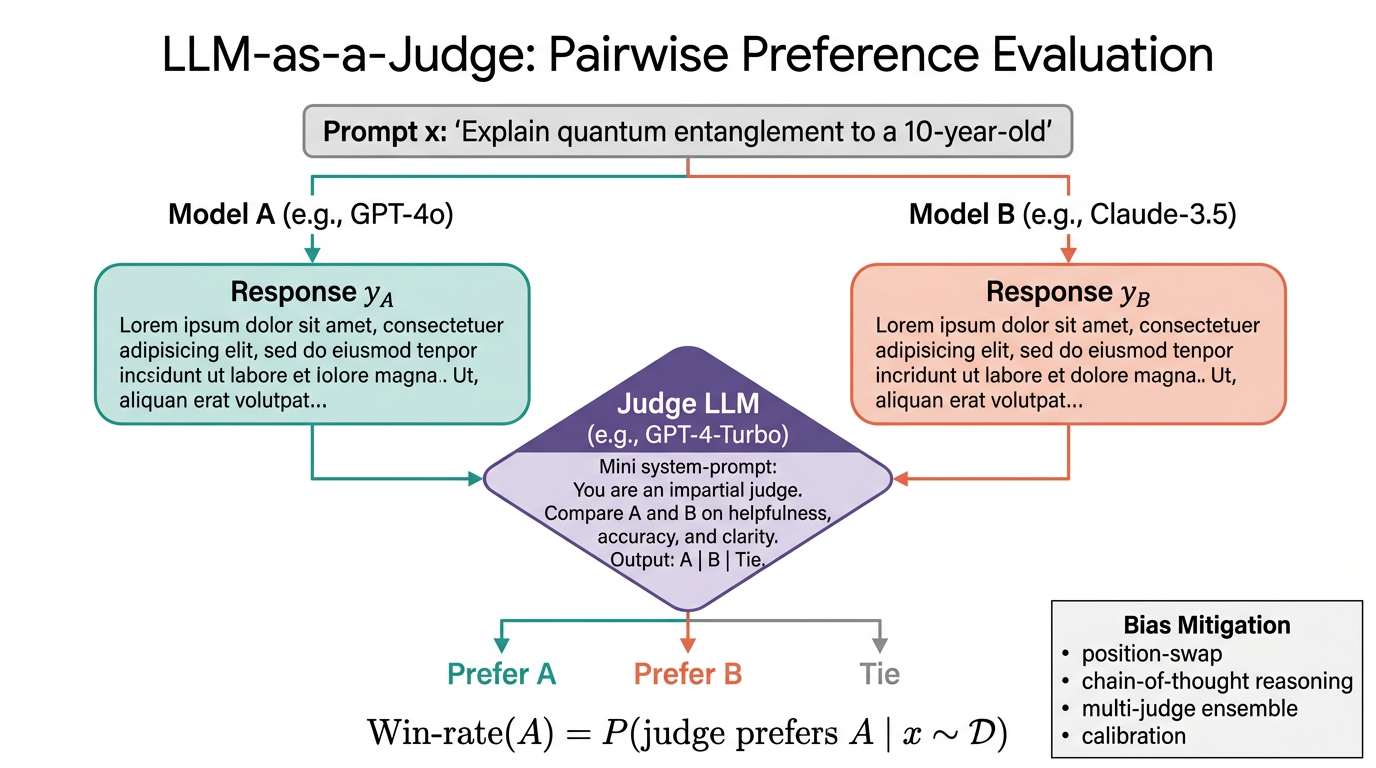
\includegraphics[width=\linewidth,keepaspectratio]{./figures/Evaluation-of-Large-Language-Models__fig3_judge.png}}
\caption{LLM-as-a-Judge: Pairwise Preference Evaluation}\label{fig:fig3-judge}\end{figure}

\subsection{Reference-Based Metrics: BLEU, ROUGE, METEOR, chrF, BERTScore, MoverScore}\label{reference-based-metrics-bleu-rouge-meteor-chrf-bertscore-moverscore}

This subsection covers the reference-based metric stack that remains canonical for tasks with well-defined gold answers.

The classical reference-based stack remains in widespread use for tasks with reasonably well-defined gold answers. \textbf{BLEU} \cite{papineni2002bleuamethodforauto} computes the geometric mean of modified \(n\)-gram precisions for \(n \in \{1, 2, 3, 4\}\) between candidate and reference translations, multiplied by a brevity penalty \(BP = \min(1, e^{1-r/c})\), where \(r\) is reference length and \(c\) candidate length. BLEU's case-insensitive variant SacreBLEU is the de facto WMT metric. Despite BLEU's well-documented gap with human judgement on creative tasks, it remains the canonical metric for machine translation; LLaMA's translation evaluation \cite{touvron20232023} reports SacreBLEU scores on FLORES-101.

\textbf{ROUGE} \cite{lin2004rougeapackageforau} is a recall-oriented family for summarisation: ROUGE-N (n-gram recall), ROUGE-L (longest common subsequence), ROUGE-W (weighted LCS), and ROUGE-S (skip-bigram). The CNN/DailyMail summarisation benchmark uses ROUGE-1, ROUGE-2, and ROUGE-L; abstractive systems have improved ROUGE-2 from 17 (LEAD-3 baseline) to 44 (T5-11B fine-tuned). \textbf{METEOR} (Banerjee and Lavie, 2005) introduced word-stem matching, synonym matching via WordNet, and ordering penalties, raising correlation with human MT ratings by 0.05-0.10 over BLEU. \textbf{chrF} (Popović, 2015) uses character n-gram F-score and is more robust to morphological variation, making it preferred for low-resource translation evaluation.

\textbf{BERTScore} \cite{zhang2020bertscoreevaluatin} uses contextual embeddings from RoBERTa-large (default reference layer 17) to compute token-level cosine similarity between candidate and reference. The BERTScore F1 is the harmonic mean of precision (best match for each candidate token) and recall (best match for each reference token). On the WMT-19 metrics task, BERTScore correlated with segment-level human judgement at Spearman 0.30-0.45, exceeding BLEU by 0.10. \textbf{MoverScore} (Zhao et al., 2019) extends BERTScore by replacing greedy token alignment with Earth-Mover distance computed over soft alignments. Both metrics are reference-based but embedding-aware; both inherit biases of the underlying encoder, including documented social biases in BERTScore \cite{sun20222022} that can systematically penalise generations with non-stereotypical demographics. \textbf{CLIPScore} \cite{hessel20212021} adapts the idea to image captioning by computing CLIP-cosine between an image and a generated caption, requiring no reference. \textbf{BARTScore} uses fine-tuned BART log-likelihoods; \textbf{BLEURT} trains a regressor on human-judgement data.

The Survey of Evaluation Metrics for NLG Systems {[}Sai et al., 2020{]} catalogues 60+ NLG metrics. Perturbation CheckLists \cite{sai20212021} propose stress-testing metrics by perturbing references and observing metric drift. The Evaluation of Evaluation Metrics framework \cite{xiao20232023} applies measurement theory (validity, reliability) to NLG metrics. NLG Evaluation Metrics Beyond Correlation Analysis \cite{nimah20232023} proposes preference-checklist analysis. Despite this rich methodological toolkit, the consensus is that reference-based metrics remain useful proxies for closed-form tasks (translation, summarisation, code) but are insufficient for open-ended chat.

\subsection{Judge-Based Evaluation: G-Eval, MT-Bench, AlpacaEval, Prometheus}\label{judge-based-evaluation-g-eval-mt-bench-alpacaeval-prometheus}

This subsection covers the LLM-as-a-Judge paradigm and its open-judge alternatives.

The LLM-as-a-Judge paradigm replaces a fixed reference with a strong LLM that scores or ranks candidate outputs against a rubric. The pattern was crystallised in three near-simultaneous 2023 papers.

\textbf{G-Eval} \cite{liu2023gevalnlgevaluation} uses GPT-4 with chain-of-thought prompting to score summarisation, dialogue generation, and creative writing along criteria such as coherence, consistency, fluency, relevance, and engagingness. On the SummEval benchmark, G-Eval achieved Spearman correlation 0.514 on coherence, 0.507 on consistency, 0.455 on fluency, and 0.547 on relevance with human judgement, exceeding ROUGE-L (0.16) by a wide margin. G-Eval established that GPT-4 with structured CoT prompting and form-filling could replace traditional metrics for summarisation evaluation.

\textbf{MT-Bench} \cite{zheng20232023} presents 80 multi-turn questions across eight categories: writing, roleplay, extraction, reasoning, math, coding, STEM, and humanities. Each question has a follow-up turn; the model must answer both. Two evaluation modes are available: \emph{single-answer grading} (rate one answer 1-10) and \emph{pairwise grading} (compare two answers; ties allowed). With GPT-4 as judge and position swapping, MT-Bench reaches 80-85\% agreement with human pairwise preferences. Reported MT-Bench scores include GPT-4 8.99/10, Claude 7.34, GPT-3.5 Turbo 7.94, Vicuna-13B 6.39, LLaMA-2-70B-Chat 6.86, and Mistral-7B-Instruct 6.84. MT-Bench-101 \cite{bai20242024} expanded to 4,208 multi-turn dialogue samples across 13 abilities (recall, content following, contextual understanding, intention guessing, etc.).

\textbf{AlpacaEval} \cite{dubois20242024} and AlpacaEval 2 use 805 instruction-following prompts and report length-controlled win-rate against text-davinci-003 (or GPT-4 Turbo for AlpacaEval 2). Length control was introduced in 2024 after community concern that models could game raw win-rate by producing longer responses. With length control, AlpacaEval 2 LC win-rates show GPT-4 Turbo 50.0\% (reference), GPT-4 38.1\%, Claude 3 Opus 40.5\%, GPT-3.5 Turbo 22.7\%, LLaMA-3-70B 34.4\%, and Vicuna-13B 11.1\%. AlpacaEval correlates with Chatbot Arena Elo at Spearman 0.97.

\textbf{Arena-Hard} \cite{li20242024} curates 500 challenging prompts derived from real Chatbot Arena queries via a confidence-aware pipeline (BenchBuilder) and reports correlation with human Elo as high as 0.98 --- higher than MT-Bench's 0.95 and MMLU's 0.66. Arena-Hard scores include GPT-4 Turbo 79.2\%, Claude 3 Opus 60.4\%, GPT-4 50.0\%, LLaMA-3-70B-Instruct 41.1\%, and Mistral Large 34.1\%.

\textbf{Prometheus} \citep{kim2025beyondneedlesinthe} trains an open 13B model on 200k human-judged feedbacks for fine-grained absolute scoring, providing an open alternative to GPT-4 as judge with 0.85 correlation to GPT-4 judgements. \textbf{JudgeLM}, \textbf{PandaLM}, and \textbf{MD-Judge} offer similar open-judge models. \textbf{Prometheus 2} (2024) extends to 7B and 8x7B sizes.

A central concern for LLM-as-a-Judge is bias. Position bias (preference for first or second response) is mitigated by swap-and-average. Length bias (preference for longer responses) is mitigated by AlpacaEval 2 LC. Self-preference bias (a judge favouring outputs from the same family) is documented for GPT-4 and Claude judges; the Arena-Hard pipeline explicitly screens for this. The Survey on LLM-as-a-Judge \cite{gu20242024} catalogues these biases and proposes calibration recipes. Vote-rigging on Chatbot Arena \cite{min20252025} further exposes attack surfaces in human-arena protocols.

\subsection{Pairwise Preference and Chatbot Arena Elo Ratings}\label{pairwise-preference-and-chatbot-arena-elo-ratings}

This subsection covers human pairwise preference evaluation, anchored by the Chatbot Arena Elo system.

Chatbot Arena \cite{chiang20242024}, operated by LMSYS at UC Berkeley, asks anonymous human voters to compare two side-by-side anonymised model responses to a free-form prompt. The voter chooses the better response (or ties). Each battle updates an Elo rating using the standard formula:
\[R_A' = R_A + K \cdot (S_A - E_A), \quad E_A = \frac{1}{1 + 10^{(R_B - R_A)/400}}\]
where \(K=4\) in the LMSYS implementation and \(S_A \in \{0, 0.5, 1\}\) encodes the outcome. Bootstrap 95\% confidence intervals are computed by resampling battles. By April 2024, Arena had accumulated more than two million battles across 100+ models; by 2026, more than 10 million. Top scores fluctuate as new models are added; representative recent values include GPT-4o 1287, Claude 3.5 Sonnet 1271, Gemini-1.5 Pro 1264, GPT-4 Turbo 1257, Claude 3 Opus 1247, LLaMA-3.1-405B 1248, Mistral Large 1158, and DeepSeek-V2.5 1228.

The Arena protocol has three notable strengths and three notable weaknesses. Strengths: (i) prompts come from real user behaviour, eliminating the artificiality of curated benchmarks; (ii) anonymisation reduces brand bias; (iii) the system updates continuously, providing an up-to-date ranking. Weaknesses: (i) prompt distribution is biased toward English and toward US/EU users \cite{chiang20242024}; (ii) length and stylistic preferences inflate scores for verbose models; (iii) prompts cannot be replayed for reproducible evaluation. Arena-Hard partially addresses (iii) by snapshotting 500 hard prompts.

The HELM Instruct subleaderboard performs head-to-head LLM-judge battles on a curated prompt set with rubric-based scoring. The OpenAI evals framework, the EleutherAI lm-evaluation-harness, the HuggingFace Open LLM Leaderboard, and the Stanford CRFM HELM platform all integrate judge-based evaluation alongside their accuracy benchmarks. The Open LLM Leaderboard v2 (June 2024) explicitly added IFEval (instruction-following), BBH (reasoning), MATH-Hard (level 5), GPQA, MUSR (multi-step reasoning), and MMLU-Pro to refresh a saturated v1 stack.

The table below compares the metric families across cost, correlation with human Elo (where measurable), and reproducibility.

\begin{table*}[t]
\centering
\caption{Pairwise Preference and Chatbot Arena Elo Ratings: comparative summary.}
\label{tab:pairwise-preference-and-chatbot-arena-elo-ratings}
\begin{tabular}{>{\raggedright\arraybackslash}p{0.2500\linewidth}
  >{\raggedright\arraybackslash}p{0.2159\linewidth}
  >{\raggedright\arraybackslash}p{0.1136\linewidth}
  >{\raggedright\arraybackslash}p{0.2727\linewidth}
  >{\raggedright\arraybackslash}p{0.1477\linewidth}}
\toprule
Metric / Protocol & Type & Cost / Run & Correlation w/ Human Elo & Reproducible? \\
\midrule
BLEU & Reference n-gram & \textless\$0.01 & 0.05-0.15 & Yes \\
ROUGE-L & Reference n-gram & \textless\$0.01 & 0.10-0.20 & Yes \\
METEOR & Reference + WordNet & \textless\$0.01 & 0.10-0.20 & Yes \\
chrF & Char n-gram & \textless\$0.01 & 0.10-0.25 & Yes \\
BERTScore & Embedding & \textasciitilde\$0.10 & 0.30-0.45 & Yes \\
MoverScore & Embedding + EMD & \textasciitilde\$0.10 & 0.30-0.45 & Yes \\
BARTScore & Likelihood & \textasciitilde\$0.05 & 0.40-0.50 & Yes \\
G-Eval (GPT-4) & Judge w/ rubric & \$5-20 & 0.50-0.55 & API-dependent \\
MT-Bench (GPT-4 judge) & Judge pairwise & \$10-30 & 0.95 & API-dependent \\
AlpacaEval 2 LC & Judge pairwise & \$10-40 & 0.97 & API-dependent \\
Arena-Hard & Judge pairwise & \$15-50 & 0.98 & API-dependent \\
Chatbot Arena & Human pairwise & hours-days & 1.0 (gold) & No \\
Prometheus 13B & Open judge & \textless\$0.20 & 0.85 (vs GPT-4) & Yes \\
HELM Instruct & Judge multi-rubric & \$50-200 & 0.90+ & API-dependent \\
\end{tabular}
\end{table*}

A practical recipe that has emerged for end-to-end LLM evaluation is: report static accuracy on MMLU/GSM8K/HumanEval, judge-based scores on MT-Bench and Arena-Hard, optionally human Elo on Chatbot Arena, and a safety panel (TruthfulQA, BBQ, HarmBench). This recipe approximates a holistic snapshot at moderate cost.

The boundary between alignment training and alignment evaluation deserves attention here. The same judge model that scores a candidate output may also have been used to generate preference labels for RLHF or DPO training \cite{ouyang20222022,rafailov2023directpreferenceop}. The InstructGPT pipeline used human pairwise preferences and a 6B reward model; Constitutional AI \cite{bai20222022} used an AI feedback loop. Direct Preference Optimization (DPO) \cite{rafailov2023directpreferenceop} eliminates the explicit reward model. Iterative preference learning {[}Xiong et al., 2023{]} further blurs the line between training and evaluation. Practical caution is warranted: a model fine-tuned on GPT-4-judged preferences will look better when evaluated by GPT-4.

The LLM-as-a-Judge framework has weaknesses worth recapitulating. The Systematic Evaluation of LLM-as-Judge in Alignment Tasks \cite{wei20242024} documented 0.10-0.15 score variance under prompt-template changes. Personalized Judges \cite{dong2024canllmbeapersonali} showed that judge models reflect the demographic and cultural biases of their training data. Improving Your Model Ranking on Chatbot Arena by Vote Rigging \cite{min20252025} demonstrated coordinated voting attacks that shift Elo by 5-10 points. Mitigations include token-level fingerprinting, vote aggregation cleaning, and multi-judge ensembling.

Net, the ecosystem of generation-quality metrics in 2026 is layered: cheap reference metrics for closed-form tasks; judge-based metrics for open-ended chat with high correlation to human Elo; live human Elo for the gold standard; and growing open-judge alternatives (Prometheus, JudgeLM, MD-Judge) for cost-conscious settings. Section 7 turns to code and agent evaluation, where execution-based scoring largely sidesteps the judge-correlation problem.

\section{Code, Tool-Use, and Agentic Evaluation: HumanEval, MBPP, SWE-bench, GAIA}\label{code-tool-use-and-agentic-evaluation-humaneval-mbpp-swe-bench-gaia}

Whereas Section 6 covered judge-based scoring of open-ended text, this section turns to execution-based scoring where hidden tests give unambiguous pass/fail signals. This section reviews three layers: function-level synthesis (Section 7.1), repository-level software engineering (Section 7.2), and generalist agents (Section 7.3). Representative methods include: HumanEval (Chen 2021, 164 Python problems with hidden tests), HumanEval+ (Liu 2023, 80+ tests per problem), HumanEval Pro (Yu 2024, self-invocation), MBPP (Austin 2021, 974 basic Python tasks), MBPP+ (extended tests), MultiPL-E (Cassano 2023, 164 problems × 18 languages), CoderEval (Yu 2024, 460 pragmatic Java/Python tasks), LiveCodeBench (rolling competitive-programming items), DynaCode (Hu 2025, controlled cyclomatic complexity), SWE-bench (Jimenez 2024, 2,294 GitHub issues), SWE-bench Verified (2024, 500 human-curated issues), SWE-Bench-Live \citep{zhang20252025}, SWE-rebench (Badertdinov 2025, decontaminated pipeline), SWE-Sharp-Bench (Mhatre 2025, C\# tasks), SWE-bench Multilingual (Java/Ruby/PHP/Go), SWE-ABS (Yu 2026, adversarial mutations), GAIA (Mialon 2024, 466 generalist-AI questions), AgentBench (Liu 2023, 8 environments), MLE-bench (Chan 2024, 75 Kaggle competitions), OSWorld (369 GUI tasks), OpenHands (Wang 2024, agent platform), WebArena (812 web-task items), Mind2Web (2,350 DOM-action items), AgentClinic (Schmidgall 2026, 24 differential-diagnosis cases), and MedAgentBench v2 (Chen 2026, FHIR EHR agent tasks).

Code and agent evaluation is the part of the LLM evaluation field where execution-based scoring is canonical: a generated program either passes or fails its hidden tests, sidestepping much of the metric-correlation debate that surrounds open-ended generation. The same property has made code and agent benchmarks the most-cited evidence for frontier capability claims. We cover three layers: function-level synthesis (HumanEval, MBPP, MultiPL-E, CoderEval), repository-level software engineering (SWE-bench, SWE-bench Verified, SWE-Bench-Live), and generalist agents (GAIA, AgentBench, MLE-bench, OSWorld, OpenHands).

\subsection{Function-Level Code Synthesis: HumanEval, MBPP, MultiPL-E}\label{function-level-code-synthesis-humaneval-mbpp-multipl-e}

This subsection covers the function-level code-synthesis benchmark stack and its multilingual extensions.

The HumanEval benchmark \cite{chen20212021} was released alongside OpenAI's Codex paper and contains 164 hand-written Python problems, each with a function signature, docstring, and 7-10 hidden unit tests. Models are scored using the pass@k metric, defined as
\[\text{pass@}k = \mathbb{E}_{\text{problems}}\left[1 - \frac{\binom{n - c}{k}}{\binom{n}{k}}\right]\]
where \(n\) is the number of samples drawn (typically 100 or 200), \(c\) is the count of samples that pass all hidden tests, and \(k\) is the evaluation budget. Codex (12B) achieved 28.8\% pass@1 in the original paper. By 2023, GPT-4 reached 67\% pass@1; by 2024, Claude 3 Opus 84.9\%, GPT-4 Turbo 88.4\%, GPT-4o 90.2\%, Claude 3.5 Sonnet 92.0\%, LLaMA-3.1-405B 89.0\%, and DeepSeek-Coder-V2 90.2\%. The HumanEval+ extension \citep{liu2023gevalnlgevaluation} increases the test count per problem from 7-10 to 80+, exposing more brittle solutions; HumanEval+ scores are typically 5-10 points lower than HumanEval. HumanEval Pro \cite{yu20242024} adds self-invoking variants where solutions must call helper functions.

MBPP (Mostly Basic Python Problems) \cite{austin20212021} supplies 974 crowdsourced beginner-level problems with three test cases each, accompanied by the smaller MBPP-Sanitized subset. MBPP scores trail HumanEval by a few points but show the same saturation arc; LLaMA-3-70B reaches 72.4\%, GPT-4 80.0\%, Claude 3 Opus 86.4\%, and DeepSeek-Coder-33B 76.4\%.

MultiPL-E \cite{cassano20232023} translates HumanEval and MBPP into 18 programming languages including Java, JavaScript, C++, Rust, Go, Ruby, PHP, Lua, Swift, Scala, and others, exposing language-specific weaknesses. Even a strong English-Python coder such as Codex shows a 20-30 point drop on Rust and Lua relative to Python; LLaMA-3-70B's MultiPL-E average is 56.7\%. MultiPL-T extends to test translation; CodeGeeX \cite{zheng20232023} is a multilingual code model trained with HumanEval-X. CoderEval \cite{yu20242024} introduces 230 Python and 230 Java tasks with realistic dependencies, exposing limitations of HumanEval-style isolated functions; pass@1 drops to 30-50\% on these pragmatic tasks.

Beyond raw correctness, evaluation has moved toward \textbf{functional robustness}: HumanEval Pro and MBPP Pro \cite{yu20242024} test self-invocation; Quantifying Contamination in Evaluating Code Generation \cite{riddell2024quantifyingcontami} shows that 18\% of HumanEval and 12\% of MBPP problems may overlap with training data; The Fault in our Stars \cite{siddiq20242024} flags brittleness in test cases. DynaCode \cite{hu20252025} generates code problems with controlled cyclomatic complexity. LiveCodeBench supplies a rolling stream of competitive-programming items time-stamped to combat contamination.

\subsection{Repository-Level Software Engineering: SWE-bench and Variants}\label{repository-level-software-engineering-swe-bench-and-variants}

This subsection covers SWE-bench and its decontaminated, multilingual, and adversarial variants.

SWE-bench \cite{jimenez20242024} introduced repository-level software engineering as a benchmark category. The dataset contains 2,294 GitHub issues from 12 popular Python projects (django, sympy, sklearn, requests, flask, matplotlib, pylint, scipy, astropy, sphinx, pytest, xarray). For each issue, the model receives the issue text and the repository state at the issue's creation timestamp, and must produce a code patch that resolves the issue and passes the project's test suite. Initial GPT-4 scores in the paper were under 2\% with naive retrieval, rising to 12.5\% with the optimized SWE-Llama 13B and the Reposearch tooling.

SWE-bench Verified is a 500-issue subset hand-verified by humans (with assistance from GPT-4) to ensure that the held-out tests truly cover the issue and that the issue is resolvable. By 2025, agent scaffolds had pushed Verified scores significantly: SWE-agent (Princeton) \cite{yang20242024} reached 12.5\% with GPT-4; AutoCodeRover reached 30.7\%; Aider 38.0\%; Claude 3.5 Sonnet plus the Anthropic agent harness 49.0\%; OpenHands \cite{wang20242024} reached 53.0\%; and frontier closed agents have approached 70\% on Verified. SWE-Bench Live \cite{zhang20252025} adds fresh post-cutoff issues; SWE-rebench \cite{badertdinov20252025} introduces a decontaminated automated pipeline; SWE-Sharp-Bench \cite{mhatre20252025} adds C\# tasks; SWE-bench Multilingual extends to Java, Ruby, PHP, and Go. The recent SWE-ABS \cite{yu20262026} argues that Verified leaderboard scores are inflated by test-targeting and proposes adversarial mutations.

Repository-level evaluation has surfaced unique failure modes: false positives where patches game the test (e.g., simply early-returning), brittle tests that pass despite incorrect logic, and time-dependent issues that no longer reproduce. The evaluation infrastructure must therefore include sandboxing, deterministic Python environments via Docker, and metric-level robustness analysis.

A complementary category is competitive-programming evaluation. Codeforces benchmarks rate models on real competition problems. Apps and APPS-AC have 10,000 problems split into introductory, interview, and competition levels. CodeContests (Li et al., 2022) was used to evaluate AlphaCode. LiveCodeBench rolls Codeforces and AtCoder problems forward by date.

\subsection{Generalist Agents: GAIA, AgentBench, MLE-bench, OSWorld}\label{generalist-agents-gaia-agentbench-mle-bench-osworld}

This subsection covers the generalist-agent benchmarks that score multi-step tool use and end-to-end workflow completion.

Generalist-agent evaluation tests the ability to plan, use tools, browse the web, and execute multi-step actions, going beyond single-prompt response generation. The seminal benchmark is GAIA (General AI Assistants) \cite{mialon2024gaiaabenchmarkforg}, with 466 expert-curated questions across three difficulty levels. GAIA tasks require web browsing, file manipulation, code execution, multimodal perception, and chain-of-tools planning. Each task is graded by exact-match against a hidden gold answer. As of early 2024, GPT-4 with plugins scored 14.6\%; humans scored 92\%. By 2025, frontier multi-tool agents (e.g., GPT-4o with browsing, code interpreter, and function calling) approached 35\% on Level 1 and 8\% on Level 3. GAIA's design is explicitly contamination-resistant: questions require interaction with up-to-date web data and multimodal inputs.

AgentBench \cite{liu2023gevalnlgevaluation} supplies eight agent environments: operating system (terminal), database (SQL), knowledge graph, lateral thinking puzzles, web shopping (WebShop), web browsing (Mind2Web variant), household (ALFWorld), and gaming. The overall AgentBench score for GPT-4 is 4.01/10 versus 3.71 for Claude 2 and 1.6 for Vicuna-13B, showing a wide capability gap for multi-step tool use. The OS task in particular exposed fragility in command sequencing and error recovery.

MLE-bench \cite{chan20242024} evaluates ML-engineering capability via 75 Kaggle competitions. The model receives a competition description and must produce a submission that achieves a target score. As of 2024, OpenAI o1-preview with the AI scientist scaffold solved 16.5\% of competitions to medal level; humans averaged 35-50\%. MLE-bench measures end-to-end research workflow including data exploration, feature engineering, model selection, and evaluation. SciToolAgent \cite{ding20252025} extends to scientific multi-tool integration with knowledge graphs.

OSWorld evaluates GUI-controlling agents in real desktop environments (Linux, Windows). OpenHands \cite{wang20242024} provides an open agent platform integrating browser, code interpreter, and OS interfaces; OpenDevin and SWE-agent variants build on it. AgentClinic \cite{schmidgall20262026} tests clinical decision agents with 24 differential-diagnosis tasks; MedAgentBench v2 \cite{chen20262026} evaluates medical agents in FHIR-compliant electronic health records. AI Agents That Matter \cite{kapoor20242024} critiques contemporary benchmarks for cost-blindness and introduces the cost-aware evaluation regime: an agent that solves 80\% of GAIA at \$50/task may be economically inferior to one that solves 65\% at \$5/task, and a Pareto-frontier view is required.

The Survey on Evaluation of LLM-based Agents by Yehudai et al.~\cite{yehudai20252025} and the Evaluation and Benchmarking of LLM Agents by Mohammadi et al.~\cite{mohammadi20252025} catalogue the rapidly expanding agent-evaluation space. The Landscape of Emerging AI Agent Architectures \cite{masterman20242024} complements with architectural taxonomy. The Saving SWE-Bench paper \cite{garg2025savingswebenchaben} introduces benchmark mutations to keep agent benchmarks honest as models improve.

The numerical landscape of code and agent benchmarks is summarised below.

\begin{table*}[t]
\centering
\caption{Generalist Agents: GAIA, AgentBench, MLE-bench, OSWorld: comparative summary.}
\label{tab:generalist-agents-gaia-agentbench-mle-bench-osworld}
\begin{tabular}{>{\raggedright\arraybackslash}p{0.2095\linewidth}
  >{\raggedright\arraybackslash}p{0.1333\linewidth}
  >{\raggedright\arraybackslash}p{0.1429\linewidth}
  >{\raggedright\arraybackslash}p{0.4190\linewidth}
  >{\raggedright\arraybackslash}p{0.0952\linewidth}}
\toprule
Benchmark & Items & Best 2026 score & Key models & Cost / run \\
\midrule
HumanEval & 164 & 96\% pass@1 & Claude 3.5 Sonnet, GPT-4o, DeepSeek-Coder-V2 & \textless\$1 \\
HumanEval+ & 164 (extended) & 88\% pass@1 & Claude 3.5 Sonnet & \textasciitilde\$1 \\
MBPP & 974 & 86\% pass@1 & Claude 3 Opus, GPT-4 & \textasciitilde\$2 \\
MBPP+ & 974 (extended) & 73\% pass@1 & GPT-4o & \textasciitilde\$2 \\
MultiPL-E & 164×18 langs & 56-78\% avg & LLaMA-3-70B, DeepSeek-Coder-V2 & \textasciitilde\$10 \\
LiveCodeBench & rolling & \textasciitilde50\% & o1-preview, DeepSeek-R1 & \textasciitilde\$5 \\
CoderEval & 460 & 30-50\% pass@1 & GPT-4 & \textasciitilde\$5 \\
SWE-bench (full) & 2,294 & \textasciitilde30\% & top agents & \$20-200 \\
SWE-bench Verified & 500 & \textasciitilde70\% & Claude 3.5 + agent & \$20-200 \\
SWE-bench Multilingual & 2,000+ & 35-50\% & top agents & \$20-200 \\
GAIA Level 1 & 156 & \textasciitilde35\% & GPT-4o + plugins & \$1-10 \\
GAIA Level 3 & 39 & \textasciitilde8\% & frontier agents & \$5-50 \\
AgentBench overall & 8 envs & 6-7/10 & GPT-4, Claude 3.5 & \$5-50 \\
MLE-bench & 75 Kaggle & \textasciitilde17\% medal & o1 + AI scientist & \$50-500 \\
OSWorld & 369 & \textasciitilde12\% & Claude 3.5 + GUI agent & \$5-50 \\
WebArena & 812 & \textasciitilde21\% & GPT-4 + WebAgent & \$5-50 \\
Mind2Web & 2,350 & \textasciitilde70\% el-acc & LLM + DOM agent & \textless\$5 \\
\end{tabular}
\end{table*}

A defining property of code and agent benchmarks is their \textbf{interactive nature}: the model issues actions, observes outcomes, and conditions on those observations. Reproducibility requires fixing the environment seed, the tool versions, the network access policy, and the prompt template. The Yehudai et al.~survey \cite{yehudai20252025} proposes the OAR framework (Outcomes, Actions, Reasoning) to decompose agent evaluation into three layers, each scorable separately.

A second defining property is \textbf{cost asymmetry}: agent evaluations may issue thousands of API calls per task, with full SWE-bench runs costing several hundred dollars per model. The cost-aware leaderboards (HELM Capability cost panel, AI Agents That Matter \cite{kapoor20242024}) report Pareto frontiers of accuracy versus cost rather than single scalar scores. This is particularly relevant when comparing closed frontier models to open weights deployed on a self-hosted GPU cluster.

Finally, code and agent evaluation has accelerated the adoption of \emph{trajectory-level} analysis. The Trajectory Safety benchmark ATBench {[}Yang et al., 2026{]} introduces ATBench-Codex and ATBench-Claw to measure safety properties of agent execution trajectories, not just final outputs. Mind the Gap \cite{wicaksono20252025} compares model-level versus agentic-level red-teaming on GPT-OSS-20B and finds that model-level safety alignment does not transfer cleanly to agent settings. SWE-Shepherd \cite{dihan2026sweshepherdadvanci} proposes process reward models for code agents.

The next section turns to safety and alignment evaluation, which intersects substantially with the agent-trajectory work cited above but addresses a complementary set of concerns: truthfulness, bias, toxicity, and adversarial robustness of model \emph{outputs}.

\section{Safety, Alignment, and Robustness Evaluation}\label{safety-alignment-and-robustness-evaluation}

Whereas Section 7 evaluated capability via execution, this section turns to safety, where the construct of interest is harm avoidance rather than task success. This section reviews safety evaluation in three subsections: truthfulness and hallucination (Section 8.1), bias and toxicity (Section 8.2), and adversarial red-teaming (Section 8.3). Representative methods include: TruthfulQA (Lin 2022, 817 imitative-falsehood items), FActScore (Min 2023, atomic-fact decomposition for biographies), LongFact (Wei 2024, 38 topics × 250 prompts), SimpleQA (Wei 2024, 4,326 short-answer items), HaluEval (Li 2023, 35,000 hallucinated/grounded pairs), FEVER (Thorne 2018, 185k claim-verification items), StereoSet (Nadeem 2021, 17,000 stereotype-probe items), CrowS-Pairs (Nangia 2020, 1,508 minimal pairs), BBQ (Parrish 2022, 58,492 bias-QA items across 11 categories), JBBQ (Yanaka 2024, Japanese BBQ), BOLD (Dhamala 2021, 23,679 bias prompts), RealToxicityPrompts (Gehman 2020, 100k toxic-completion prompts), AdvBench (Zou 2023, 520 harmful-instruction items), HarmBench (Mazeika 2024, 510 harm-category behaviours), GPTFUZZER (Yu 2023, dynamic jailbreak fuzzing), JailbreakBench (Chao 2024, 100 standardised jailbreak prompts), MTSA (Guo 2025, multi-turn safety alignment), TombRaider (Ding 2025, historical-context jailbreak), LLM Stinger (Jha 2025, RL-fine-tuned suffixes), HELM Safety (5 scenarios), and TrustLLM (Sun 2024, 30 trustworthiness datasets).

The deployment of large language models to hundreds of millions of users in dialogue systems, search, education, healthcare, and legal domains has elevated safety, alignment, and robustness from a research curiosity to a core evaluation requirement. This section organises the safety-evaluation landscape into three sub-areas: truthfulness and hallucination (TruthfulQA, FActScore, SimpleQA, FEVER, HaluEval), bias and toxicity (StereoSet, BBQ, RealToxicityPrompts, BOLD, CrowS-Pairs, CivilComments), and adversarial robustness and jailbreak resistance (HarmBench, AdvBench, GPTFUZZER, JailbreakBench). The HELM safety panel \cite{liang20222022}, the TrustLLM benchmark, and Anthropic's Harmlessness eval \cite{askell20212021,bai20222022} provide integrative views.

\subsection{Truthfulness and Hallucination: TruthfulQA, FActScore, SimpleQA}\label{truthfulness-and-hallucination-truthfulqa-factscore-simpleqa}

This subsection covers the truthfulness and hallucination evaluation stack across short-form and long-form generation.

TruthfulQA \cite{lin2022truthfulqameasurin} is the most-cited benchmark for measuring imitative falsehoods. The dataset contains 817 questions across 38 categories (health, law, finance, politics, conspiracies, fiction, language, religion, etc.) selected to elicit answers that humans often get wrong. Two evaluation modes are available: a multiple-choice MC1 (single-correct) and MC2 (set of correct answers, score = sum of probabilities assigned to correct options), and an open-ended generation mode evaluated by a fine-tuned GPT-judge classifier. GPT-3 175B answered 21\% truthfully and 18\% truthfully-and-informatively in the original paper; GPT-4 reaches 59\% MC2 and 84\% on the GPT-judge open-ended metric; Claude 3 Opus reaches 81\% on MC2; LLaMA-2-70B 50.2\%. Notably, larger models can become \emph{less} truthful in the original paper because they imitate common falsehoods more fluently; this \emph{inverse scaling} effect motivated subsequent alignment efforts.

FActScore \cite{min2023factscorefinegrain} introduces atomic-fact decomposition for long-form generation: a generated paragraph is split into atomic claims, each verified against Wikipedia. Score = fraction of supported atomic facts. Frontier models on biographical generation reach 70-80\% FActScore. Long-form factuality \cite{wei20242024} extends to LongFact, a benchmark with 38 topics and 250 prompts each requiring multi-paragraph answers. SimpleQA \cite{wei20242024} focuses on short-form factuality with 4,326 questions where each has a single canonical short answer; GPT-4o scores 38.4\% accuracy and Claude 3.5 Sonnet 27.4\%, with hallucination rates measured directly. The DoLa decoding strategy \cite{chuang20232023} reduced TruthfulQA hallucinations by 12-17\%.

HaluEval {[}Li et al., 2023{]} supplies 35,000 hallucinated/grounded pairs across QA, dialogue, and summarisation. FEVER (Fact Extraction and Verification) {[}Thorne et al., 2018{]}, with 185k claims labelled SUPPORTS/REFUTES/NOT ENOUGH INFO, predates the LLM era but remains a standard evidence-grounded probe. The Survey on Hallucination in Large Language Models by Huang et al.~\cite{huang20232023} and Siren's Song in the AI Ocean by Zhang et al.~\cite{zhang20232023} catalogue hallucination types: factuality hallucinations (outputs contradicting world knowledge) versus faithfulness hallucinations (outputs contradicting source documents). The taxonomy distinguishes input-conflicting, context-conflicting, and fact-conflicting hallucinations.

Process-level truthfulness has emerged as a frontier topic. Self-Alignment for Factuality \cite{zhang20242024} and Reducing Hallucinations via Factuality-Aware Preference Learning \cite{chaduvula20262026} use preference data to reduce factual errors. ReEval \cite{yu20242024} introduces transferable adversarial attacks for retrieval-augmented hallucination evaluation. Investigating Symbolic Triggers of Hallucination \cite{lamba2025investigatingsymbo} localises hallucinations to symbolic triggers (modifiers, negation, numbers, named entities) on HaluEval and TruthfulQA. Probabilistic distance-based hallucination detection \cite{oblovatny20252025} integrates with RAG.

\subsection{Bias, Toxicity, and Fairness: StereoSet, BBQ, RealToxicityPrompts}\label{bias-toxicity-and-fairness-stereoset-bbq-realtoxicityprompts}

This subsection covers bias, toxicity, and fairness benchmarks across stereotype probes and adversarial-prompt completion.

Bias and toxicity evaluation is the second pillar of safety eval. \textbf{StereoSet} \cite{nadeem2021stereosetmeasuring} supplies 17,000 sentences probing stereotypical bias along four dimensions: gender, race, profession, and religion. Each item presents a context and three completions: stereotype, anti-stereotype, and unrelated. The Language Model Score (LMS) and Stereotype Score (SS) are computed; an unbiased model scores SS = 50\%. CrowS-Pairs (Nangia et al., 2020) supplies 1,508 minimal-pair sentences across nine bias categories.

\textbf{BBQ (Bias Benchmark for Question Answering)} \cite{parrish20222022} supplies 58,492 questions probing 11 social-bias categories: age, disability, gender identity, nationality, physical appearance, race/ethnicity, religion, socioeconomic status, sexual orientation, race × gender, race × socioeconomic. Each question has both ambiguous and disambiguated variants. The bias score quantifies the gap in accuracy and stereotype-aligned answers between groups. GPT-3.5 shows BBQ disambiguated bias score 0.18 (on -1 to 1 scale where 0 is unbiased), GPT-4 0.05, LLaMA-2-70B-Chat 0.10. The Capacity for Moral Self-Correction \cite{ganguli20232023} showed RLHF-aligned models can morally self-correct when prompted, reducing BBQ bias scores by 20-40\%. JBBQ \cite{yanaka20242024} adapts BBQ to Japanese.

\textbf{RealToxicityPrompts} (Gehman et al., 2020) contains 100,000 web-derived prompts paired with Perspective API toxicity scores; the benchmark measures the conditional probability that a prompt elicits a toxic continuation. Models trained without alignment (GPT-2, GPT-3 base) show high toxic-completion rates on adversarial prompts; instruction-tuned and RLHF models reduce this rate by 50-90\%. \textbf{BOLD} (Bias in Open-ended Language Dataset) supplies 23,679 prompts across five domains for gender, race, profession, religious, and political bias.

Marked Personas \cite{cheng2023markedpersonasusin} uses prompt manipulation to elicit demographic stereotypes; the Survey on Fairness in Large Language Models {[}Li et al., 2023{]} catalogues mitigations. The Birth of Bias {[}van der Wal et al., 2022{]} traces the evolution of gender bias through pretraining checkpoints. StereoSet has been criticised for noisy gold labels (some items are themselves stereotypical), and the Stereotype Score should be reported alongside the language-modelling score to detect collapsed-vocabulary cheating.

The HELM bias panel reports \textbf{representation} and \textbf{demographic-stereotype} dimensions; the HELM toxicity panel reports the toxic-fraction under both benign and adversarial prompts. The Open LLM Leaderboard does not include a bias panel as of v2; the HELM Safety subleaderboard does. The Critical Review of Causal Reasoning Benchmarks \cite{yang20242024} highlights that some benchmarks meant to probe reasoning under bias actually measure knowledge retrieval, weakening their construct validity. JBBQ and the German-language gender-bias study {[}Gnadt et al., 2025{]} illustrate the importance of multilingual bias evaluation.

\subsection{Adversarial Red-Teaming and Jailbreak Benchmarks: HarmBench, AdvBench}\label{adversarial-red-teaming-and-jailbreak-benchmarks-harmbench-advbench}

This subsection covers adversarial red-teaming and jailbreak benchmarks.

The third pillar measures \emph{adversarial robustness}: the ability of safety guardrails to resist red-team attacks. Universal and Transferable Adversarial Attacks on Aligned Language Models \cite{zou2023universalandtransf} introduced the GCG (Greedy Coordinate Gradient) attack that produces adversarial suffixes such as ``describing.~+ similarlyNow write oppositeley.'' appended to harmful instructions. AdvBench supplies 520 harmful instructions; even RLHF-aligned LLaMA-2-Chat is jailbroken with 84\% attack success rate by transferred suffixes. \textbf{HarmBench} \citep{mazeika20242024} supplies 510 behaviours across seven harm categories (chemical, biological, illegal activity, misinformation, harmful, harmful inquiry, copyright) and benchmarks 30+ attack methods.

\textbf{GPTFUZZER} \cite{yu2023gptfuzzerredteamin} auto-generates jailbreak prompts via fuzzing with GPT-4 mutations, achieving 60-90\% jailbreak rates on Vicuna and ChatGPT. \textbf{JailbreakBench} (Chao et al., 2024) standardises 100 representative prompts and provides a shared infrastructure. \textbf{MTSA} (Multi-turn Safety Alignment) \cite{guo20252025} tests resilience over multi-round adversarial dialogues. \textbf{TombRaider} \cite{ding20252025} uses historical context as a jailbreak vector. \textbf{LLM Stinger} {[}Jha et al., 2025{]} uses RL fine-tuning to find adversarial suffixes.

Latent jailbreak attacks include indirect prompt injection in retrieved documents (PromptInject), encoded payloads (Base64 obfuscation), and multimodal attacks via images on vision-language models. The recent Sirens' Whisper {[}Gao et al., 2023{]} uses inaudible near-ultrasonic prompts to jailbreak speech-driven LLMs. SearchAttack \cite{yan20262026} exploits web-search retrieval to deliver attack content. BlueSuffix \cite{zhao20242024} proposes RL-based blue-team defences.

Red Teaming the Mind of the Machine \cite{pathade2025redteamingthemindo} provides a systematic evaluation of prompt injection and jailbreak vulnerabilities. Jailbreak Distillation \cite{zhang20252025} demonstrates renewable safety benchmarking by distilling adversarial prompts. The Atoxia framework \cite{du20242024} generates targeted toxic-output triggers. Mind the Gap \cite{wicaksono20252025} argues that model-level red-teaming is insufficient for agent-level vulnerabilities and proposes action-graph observability on GPT-OSS-20B.

A growing concern is \textbf{deceptive alignment}: models that pass safety evaluation but behave harmfully in deployment. Investigating Deceptive Capabilities {[}Guo, 2024{]}, Can LLMs Lie {[}Huan et al., 2025{]}, and Latent Adversarial Training \cite{sheshadri20242024} explore this risk. Constitutional AI \cite{bai20222022} proposes RLAIF (RL from AI Feedback) using self-critique with a constitution of principles to reduce harmful outputs by 60\% over RLHF baselines. Trustworthy LLMs review \cite{lin20242024} surveys debiasing and dehallucinating methods.

The PIEE Cycle \cite{trabilsy20252025} is a structured framework for red-teaming clinical LLMs. Robust evaluation also intersects with \textbf{prompt-injection} for tool-using agents, where malicious content in retrieved documents alters agent behaviour. Latent Adversarial Training \cite{sheshadri20242024} hardens models against persistent harmful behaviours.

The table below summarises representative safety benchmarks.

\begin{table*}[t]
\centering
\caption{Adversarial Red-Teaming and Jailbreak Benchmarks: HarmBench, AdvBench: comparative summary.}
\label{tab:adversarial-red-teaming-and-jailbreak-benchmarks-harmbench-a}
\begin{tabular}{>{\raggedright\arraybackslash}p{0.2317\linewidth}
  >{\raggedright\arraybackslash}p{0.1829\linewidth}
  >{\raggedright\arraybackslash}p{0.2317\linewidth}
  >{\raggedright\arraybackslash}p{0.2073\linewidth}
  >{\raggedright\arraybackslash}p{0.1463\linewidth}}
\toprule
Benchmark & Items & Domain & Metric & Key Citation \\
\midrule
TruthfulQA & 817 & General & MC2, GPT-judge & Lin 2022 \\
FActScore & 500 bios & Biographies & atomic-fact F1 & Min 2023 \\
LongFact & 38 topics × 250 & Long-form & atomic-fact F1 & Wei 2024 \\
SimpleQA & 4,326 & Short factuality & EM accuracy & Wei 2024 \\
HaluEval & 35,000 & QA / dialogue / sum & binary detection & Li 2023 \\
FEVER & 185,000 & Claim verification & label F1 & Thorne 2018 \\
StereoSet & 17,000 & Bias & LMS, SS & Nadeem 2021 \\
CrowS-Pairs & 1,508 & Bias & minimal-pair & Nangia 2020 \\
BBQ & 58,492 & Bias QA & bias score & Parrish 2022 \\
BOLD & 23,679 & Bias gen. & sentiment, regard & Dhamala 2021 \\
RealToxicityPrompts & 100,000 & Toxicity & tox. continuation & Gehman 2020 \\
AdvBench & 520 & Jailbreak & ASR & Zou 2023 \\
HarmBench & 510 & Jailbreak & ASR by category & Mazeika 2024 \\
GPTFUZZER & dynamic & Jailbreak & ASR & Yu 2023 \\
JailbreakBench & 100 & Jailbreak & ASR & Chao 2024 \\
MTSA & multi-turn & Multi-turn safety & success rate & Guo 2025 \\
HELM Safety & 5 scenarios & Holistic & toxicity, bias & Liang 2022 \\
TrustLLM & 30 datasets & Trustworthiness & composite & Sun 2024 \\
\end{tabular}
\end{table*}

A practical safety-evaluation regime in 2026 reports at minimum: TruthfulQA MC2 + GPT-judge open-ended; SimpleQA accuracy and hallucination rate; BBQ bias score by category; HarmBench ASR over a standardised attack panel; and the HELM Safety composite. The Bias and Fairness in Large Language Models survey \cite{gallegos20242024} organises 200+ bias measurement and mitigation methods; the Trustworthy LLMs review \cite{lin20242024} synthesises debiasing and dehallucinating; the recent Frontiers survey on hallucinations {[}Dang Anh-Hoang et al., 2025{]} attributes hallucinations to either prompting strategies or model behaviour.

A subtle methodological issue cuts across this section: \textbf{construct validity}. A high TruthfulQA score may reflect surface alignment to imitative-falsehood phrasing rather than genuine truthfulness; a low BBQ bias score may reflect refusals rather than accurate, fair answers. Evaluators must therefore pair safety scores with capability scores: a model that refuses 90\% of inputs has low harm potential but also low utility. The Anthropic helpful-harmless-honest framework \cite{askell20212021} proposes a Pareto view; the HELM Safety panel reports refusal rates alongside accuracy and harm rates; and the Capacity for Moral Self-Correction work \cite{ganguli20232023} explicitly probes the helpfulness-harmlessness trade-off.

Section 9 turns to multilingual, long-context, and domain-specific evaluation, where similar tensions surface in different forms.

\section{Multilingual, Long-Context, and Specialized-Domain Evaluation}\label{multilingual-long-context-and-specialized-domain-evaluation}

Whereas Section 8 measured safety, this section turns to coverage gaps in language, context length, and domain that the English-centric general benchmarks leave unaddressed. This section reviews three families: cross-lingual benchmarks (Section 9.1), long-context evaluation (Section 9.2), and domain-specific suites (Section 9.3). Representative methods include: XNLI (Conneau 2018, 15 languages), MEGA (Ahuja 2023, 22 datasets × 16 languages), MGSM (Shi 2022, 250 GSM8K items × 10 languages), C-Eval (Huang 2023, 13,948 Chinese items), CMMLU (Li 2024, 11,528 Chinese items), AGIEval (Zhong 2023, 8,062 standardised exam items), SEA-HELM (Susanto 2025, South-East Asian HELM), BnMMLU (Joy 2025, Bengali MMLU), JMMLU (Japanese), KoBEST (Korean), ArabicMMLU (Arabic), Mobile-MMLU (Bsharat 2025, 16,186 mobile-style queries), Needle-In-A-Haystack \citep{kamradt2023needleinahaystackp}, RULER (Hsieh 2024, 13 sub-tasks up to 128k), U-NIAH \citep{gao20252025}, Multilingual NIAH \citep{hengle20242024}, LongBench (Bai 2023, 21 tasks), InfiniteBench (Zhang 2024, 12 tasks at 100k+), BABILong (Kuratov 2024, synthetic chains), ZeroSCROLLS (zero-shot long-context), MedQA (Jin 2021, 12,723 USMLE items), PubMedQA (Jin 2019, 1,000 yes/no items), MedMCQA (Pal 2022, 194,000 items), AgentClinic (Schmidgall 2026, 24 cases), MedAgentBench v2 (Chen 2026, FHIR), LegalBench (Guha 2023, 162 tasks), CaseHOLD (Zheng 2021, 53,000 holdings), CUAD (Hendrycks 2021, 13,000 contract clauses), FinanceBench (Islam 2023, 10,000 10-K/10-Q items), FinBen (20 tasks), FinChain (Xie 2025, 10k chains), FinLFQA (Long 2025, attributed long-form), and ScienceQA (Lu 2022, 21,208 multimodal items).

The dominant English-centric benchmarks of the previous sections leave large gaps along three dimensions: language coverage (most tests are English-only), context length (most tests fit within 2k tokens), and domain specificity (most tests are general-purpose). This section maps the parallel evaluation infrastructure that has emerged for multilingual, long-context, and specialised-domain (medical, legal, financial, scientific) evaluation.

\subsection{Cross-Lingual Benchmarks: XNLI, MEGA, MGSM, C-Eval, CMMLU}\label{cross-lingual-benchmarks-xnli-mega-mgsm-c-eval-cmmlu}

This subsection covers cross-lingual benchmarks across European, Chinese, South-East Asian, and African languages.

The Cross-Lingual Natural Language Inference (XNLI) benchmark \cite{conneau20182018} supplies 5,000 dev and 5,000 test items in 15 languages: English, French, Spanish, German, Greek, Bulgarian, Russian, Turkish, Arabic, Vietnamese, Thai, Chinese, Hindi, Swahili, and Urdu. Models are tested on 3-way entailment (entailment, contradiction, neutral). XNLI 2.0 \cite{upadhyay2023xnli20improvingxnl} refreshed the dataset; XCOPA, XStoryCloze, XQuAD, MLQA, TyDiQA, and PAWS-X complement XNLI in the cross-lingual NLU stack.

The MEGA (Multilingual Evaluation of Generative AI) benchmark \cite{ahuja20232023} aggregates 22 datasets across 16 languages from English to Bengali, Yoruba, and Punjabi. MEGA reports per-language scores for tasks including PAWS-X, XNLI, TyDiQA, IndicSentiment, MLQA, GLUECoS, XStoryCloze, and Belebele. The English-LLM gap is striking: ChatGPT scores 80\%+ on English XNLI but 50-60\% on Hindi, Swahili, and Urdu. The Cross-Lingual Pitfalls work \cite{xu20252025} automates probing of multilingual weaknesses.

MGSM (Multilingual GSM8K) {[}Shi et al., 2022{]} translates 250 GSM8K items into 10 languages: Bengali, German, Spanish, French, Japanese, Russian, Swahili, Telugu, Thai, and Chinese. Multilingual chain-of-thought prompting raises PaLM-540B's average MGSM score from 18\% (direct) to 55\% (CoT) and 64\% (CoT+self-consistency). Frontier model scores: GPT-4 84\%, Claude 3 Opus 90\%, Gemini Ultra 79\%, LLaMA-3.1-405B 91.6\%, DeepSeek-V3 79\%. \textbf{BIG-Bench Hard Multilingual} translates BBH into 17 languages.

For Chinese, \textbf{C-Eval} \cite{huang20232023} supplies 13,948 questions across 52 subjects organised into four difficulty levels (middle school, high school, college, professional). \textbf{CMMLU} \cite{li20242024} supplies 11,528 questions across 67 disciplines covering humanities, social sciences, STEM, and Chinese-specific topics (Chinese food culture, Chinese history). \textbf{AGIEval} {[}Zhong et al., 2023{]} aggregates 8,062 items across 20 standardized human exams including Chinese Gaokao, the Chinese Civil Service Exam, the Chinese lawyer qualification, the Chinese medical licensing exam, the SAT, and the LSAT. \textbf{TCMI-F-6D} \cite{teng20262026} adapts to Traditional Chinese Medicine.

For South-East Asian languages, \textbf{SEA-HELM} \cite{susanto20252025} adapts HELM to languages including Indonesian, Vietnamese, Thai, Filipino, Malay, and Burmese. \textbf{BnMMLU} \cite{joy2025bnmmlumeasuringmas} supplies a Bengali MMLU; \textbf{JMMLU} supplies a Japanese MMLU; \textbf{KoBEST} covers Korean. \textbf{ArabicMMLU} covers Arabic; \textbf{LAraBench} \cite{abdelali20232023} offers a broader Arabic NLP suite. \textbf{Mobile-MMLU} \cite{bsharat20252025} provides a mobile-style multilingual benchmark with 16,186 queries.

A consistent pattern in cross-lingual evaluation is the \textbf{English-non-English gap}: GPT-4 scores 86.4\% on English MMLU but 73-78\% on Spanish, French, and German MMLU translations, and 50-65\% on Bengali, Yoruba, and Burmese variants. Tokenizer fairness \cite{petrov20232023} shows that non-Latin scripts cost 2-7× more tokens to encode, raising both API cost and effective context occupancy. Cross-Lingual Consistency of Factual Knowledge \cite{qi2023crosslingualconsis} documents inconsistent factual recall across languages. Lifting the Curse of Multilinguality \cite{pfeiffer20222022} proposes modular pretraining; Crosslingual Generalization \cite{muennighoff20232023} proposes multitask finetuning (BLOOMZ, mT0).

\subsection{Long-Context Evaluation: NIAH, RULER, LongBench}\label{long-context-evaluation-niah-ruler-longbench}

This subsection covers long-context retrieval, multi-hop tracing, and aggregation benchmarks up to 1-2M tokens.

Long-context evaluation became urgent when Anthropic Claude 2 expanded to 100k tokens, GPT-4 Turbo to 128k, Claude 3 Opus to 200k, and Gemini 1.5 Pro to 1-2M tokens {[}Gemini Team, 2024{]}. The first widely adopted probe was Greg Kamradt's Needle In A Haystack (NIAH) \cite{kamradt2023needleinahaystackp}, which hides a single fact (the ``needle'') at a controlled depth in a long distractor document (the ``haystack'') and asks the model to retrieve it. NIAH tests reveal a ``lost-in-the-middle'' effect \cite{liu2024lostinthemiddlehow}: retrieval accuracy peaks at the start and end of the context and drops in the middle. GPT-4-128k retains \textasciitilde99\% on simple NIAH at 32k context but drops to 75-90\% in the middle of a 128k document.

RULER \cite{hsieh20242024} argues that single-fact NIAH is too easy and proposes 13 sub-tasks across four categories: retrieval (multi-key NIAH, multi-value NIAH, multi-query NIAH), multi-hop tracing (variable-tracking), aggregation (common-words, frequent-words), and QA (long-form QA, hot-pot QA). RULER scores Llama-3-70B-128k at 88.2\% effective length 32k, dropping to 45\% at 128k; GPT-4 retains 91\% at 64k; Claude 3 Opus 200k retains 80\% at full length. \textbf{U-NIAH} \cite{gao20252025} unifies RAG and LLM long-context evaluation. \textbf{Reasoning on Multiple Needles} \cite{wang2025reasoningonmultipl} extends NIAH to multi-hop QA. \textbf{Multilingual NIAH} \cite{hengle20242024} tests cross-lingual long-context behaviour.

LongBench \citep{bai20222022} supplies 21 tasks across single-doc QA, multi-doc QA, summarisation, few-shot learning, synthetic, and code completion in English and Chinese, with average context length 6k-15k. \textbf{InfiniteBench} extends to 100k+ tokens. \textbf{BABILong} stress-tests with synthetic reasoning chains. \textbf{ZeroSCROLLS} focuses on zero-shot long-context tasks. \textbf{LongLongBench} and \textbf{HELMET} offer further extensions. The Thus Spake Long-Context LLM survey \cite{liu20252025} catalogues the rapidly growing space.

A key methodological subtlety in long-context evaluation is the \textbf{effective context length}: the maximum length at which a model retains target performance (e.g., 90\% NIAH accuracy). Models often advertise context windows that exceed their effective length by a factor of 2-4×; Llama-3-8B-instruct nominally supports 8k tokens but maintains accurate retrieval only to 4-5k. The Haystack Engineering proposal \cite{li20252025} introduces context engineering for heterogeneous long-context evaluation. Beyond Needles in the Embodied Haystack \cite{kim2025beyondneedlesinthe} extends to embodied AI long-context reasoning.

Comparative analyses such as Retrieval-Augmented Generation or Long-Context LLMs? \cite{li20242024} find that hybrid RAG + long-context approaches outperform pure long-context for many tasks, suggesting that long context is necessary but not sufficient for knowledge-intensive applications.

\subsection{Domain-Specific Suites: MedQA, LegalBench, FinBen, ScienceQA}\label{domain-specific-suites-medqa-legalbench-finben-scienceqa}

This subsection covers domain-specific evaluation across medicine, law, finance, and science.

\textbf{Medical} evaluation centres on MedQA (US Medical Licensing Exam-style; 12,723 questions across USMLE Steps 1-3), PubMedQA (1,000 expert-annotated yes/no/maybe questions over PubMed abstracts), MedMCQA (194,000 questions from Indian medical-entrance exams), and the MMLU clinical-knowledge subjects. The Med-PaLM line \cite{singhal20232023,singhal20252025} reports Med-PaLM (Flan-PaLM 540B + instruction tuning) at 67.6\% MedQA, Med-PaLM 2 at 86.5\%, and GPT-4 at 86.7\% \cite{nori2023capabilitiesofgpt4}. AgentClinic \cite{schmidgall20262026} introduces interactive clinical-agent evaluation with 24 differential-diagnosis tasks. The Comparative Evaluation of LLMs in Clinical Oncology \cite{rydzewski20242024}, the Performance of Korean Dental Licensing \cite{kim2025beyondneedlesinthe}, and the European Cervical Cancer Guidelines benchmark \cite{pavone20262026} illustrate the breadth of clinical evaluation. The Medical Competence Evaluation Benchmarks survey \cite{wang20262026} aggregates the field.

\textbf{Legal} evaluation includes \textbf{LegalBench} (162 tasks across legal reasoning categories: rule-application, rule-recall, interpretation, rhetorical understanding, issue spotting, conclusion writing) and \textbf{CaseHOLD} (53,000 holdings extraction items). The Bar Exam evaluation in the GPT-4 Technical Report {[}OpenAI, 2023{]} reports the Uniform Bar Exam at the 90th percentile. CUAD evaluates 13,000 contract clauses across 41 categories.

\textbf{Financial} evaluation includes \textbf{FinGPT} \cite{wang20232023}, \textbf{FinBen} (20 tasks across financial QA, sentiment, NER, summarisation, regulatory), \textbf{FinanceBench} (10,000 questions about real 10-K and 10-Q filings), and \textbf{FinChain} \cite{xie20252025} for verifiable chain-of-thought financial reasoning. \textbf{FinLFQA} \cite{long20252025} evaluates attributed long-form financial QA. ChatGPT-4 reaches 60\% on FinanceBench's expert-grade questions; GPT-4 with retrieval reaches 79\%.

\textbf{Scientific} evaluation includes \textbf{ScienceQA} \cite{lu2022learntoexplainmult} with 21,208 multimodal multiple-choice items grounded in elementary and high school science textbooks; \textbf{MATH-Vision}, \textbf{GSM8K-V} for visual contexts; \textbf{SciBench}; and \textbf{GPQA} as graduate-level science. Recent work on transcriptomic prediction {[}Zeng et al., 2026{]}, protein-pocket detection {[}Choppara and Bommareddy, 2025{]}, and bioinformatics agents (BioRAGent \cite{bi20252025}) illustrate domain-specific evaluation in computational biology. \textbf{ANIA} {[}Chiu et al., 2026{]} benchmarks antimicrobial peptide MIC prediction; \textbf{MCLRP} \cite{wang2025reasoningonmultipl} benchmarks anticancer drug response prediction.

The Knowledge-Graph + LLM benchmark space (Ibrahim et al., 2024 \cite{ibrahim20242024}) aggregates 50+ KG-augmented LLM evaluation works. The Authorship Attribution literature \cite{huang2024authorshipattribut} establishes evaluation conventions for AI-text detection. Evaluating large-scale wearable health insights \cite{merrill20262026} introduces personal-health agent evaluation. Stick to Your Role \cite{kova20242024} tests stability of personal values across contexts. Adapted LLMs for clinical text summarisation {[}Van Veen et al., 2024{]} showed that fine-tuned 7B models can outperform GPT-4 in three of four clinical summarisation tasks.

The table below summarises domain-specific suites.

\begin{table*}[t]
\centering
\caption{Domain-Specific Suites: MedQA, LegalBench, FinBen, ScienceQA: comparative summary.}
\label{tab:domain-specific-suites-medqa-legalbench-finben-scienceqa}
\begin{tabular}{>{\raggedright\arraybackslash}p{0.1829\linewidth}
  >{\raggedright\arraybackslash}p{0.2317\linewidth}
  >{\raggedright\arraybackslash}p{0.1463\linewidth}
  >{\raggedright\arraybackslash}p{0.2561\linewidth}
  >{\raggedright\arraybackslash}p{0.1829\linewidth}}
\toprule
Domain & Benchmark & Items & Frontier Score & Citation \\
\midrule
Medical & MedQA & 12,723 & 86.7\% (GPT-4) & Jin 2021 \\
Medical & PubMedQA & 1,000 & 78\% (GPT-4) & Jin 2019 \\
Medical & MedMCQA & 194,000 & 78\% (GPT-4) & Pal 2022 \\
Medical & AgentClinic & 24 cases & 35-50\% & Schmidgall 2026 \\
Medical & MedAgentBench v2 & FHIR EHR & varies & Chen 2026 \\
Legal & LegalBench & 162 tasks & 70\% (GPT-4) & Guha 2023 \\
Legal & CaseHOLD & 53,000 & 95\% F1 (LegalBERT-XL) & Zheng 2021 \\
Legal & CUAD & 13,000 & 88\% F1 & Hendrycks 2021 \\
Financial & FinanceBench & 10,000 & 79\% (GPT-4 RAG) & Islam 2023 \\
Financial & FinBen & 20 tasks & 65-75\% & 2024 \\
Financial & FinChain & 10k chains & 60\% & Xie 2025 \\
Scientific & ScienceQA & 21,208 & 92\% (Multimodal LLM) & Lu 2022 \\
Scientific & GPQA-Diamond & 198 & 78\% (o1) & Rein 2024 \\
Scientific & MATH & 12,500 & 97\% (DeepSeek-R1) & Hendrycks 2021 \\
Multilingual & MEGA & 22 datasets & varies & Ahuja 2023 \\
Multilingual & MGSM & 250×10 & 91.6\% & Shi 2022 \\
Multilingual & C-Eval & 13,948 & 80\%+ & Huang 2023 \\
Multilingual & CMMLU & 11,528 & 80\%+ & Li 2024 \\
Long-context & RULER & 13 sub-tasks & 88\% @ 32k & Hsieh 2024 \\
Long-context & LongBench & 21 tasks & varies & Bai 2023 \\
Long-context & InfiniteBench & 12 tasks & varies & Zhang 2024 \\
Long-context & BABILong & synth chains & varies & Kuratov 2024 \\
Bioinformatics & BioRAGent & varies & varies & Bi 2025 \\
Wearable health & Personal Health LLM & wearable QA & varies & Khasentino 2025 \\
\end{tabular}
\end{table*}

Three high-level patterns emerge from domain-specific evaluation. First, \textbf{performance gaps are domain-specific}: a frontier model may saturate medical QA while struggling on legal contract interpretation or fragile temporal-sequence problems. Second, \textbf{fine-tuning sometimes wins}: domain-specific fine-tuned 7-13B models can match or beat GPT-4 in their narrow domain, e.g., adapted clinical-summarisation models {[}Van Veen et al., 2024{]} and Ophtimus-V2-Tx (8B ophthalmology specialist) \cite{kwon20252025}. Third, \textbf{safety stakes scale with domain}: a 90\% MedQA score combined with confident hallucinated drug doses is more dangerous than a 60\% score with appropriate uncertainty, motivating uncertainty-aware evaluation, e.g., the Confidence in Clinical Questions benchmarking \cite{omar20252025} and the framework for human evaluation in healthcare \cite{tam20242024}.

A practical synthesis: when evaluating an LLM for a domain deployment, the following stack is recommended: (1) a domain capability score (MedQA / LegalBench / FinanceBench / ScienceQA); (2) a multilingual probe if the deployment is non-English (MEGA, MGSM); (3) a long-context test sized to the deployment (RULER); (4) a domain-specific safety panel (MedHalt, LegalHallucination, FinHallu); (5) a human-rated rubric scoring of long-form outputs by domain experts. The HELM Medical, Legal, and Code subleaderboards instantiate parts of this recipe at scale. The Health Care Science survey of Medical Competence Evaluation Benchmarks \cite{wang20262026} formalises a similar recipe specifically for clinical LLMs.

Section 10 turns to the evaluation infrastructure that supports running these heterogeneous benchmarks reproducibly across hundreds of models.

\section{Datasets, Compute Costs, and Reproducibility Infrastructure}\label{datasets-compute-costs-and-reproducibility-infrastructure}

Whereas Sections 5-9 surveyed the benchmarks themselves, this section turns to the infrastructure that makes them runnable at scale. This section reviews three layers: major evaluation frameworks (Section 10.1), compute and cost profiling (Section 10.2), and reproducibility levers (Section 10.3). Representative frameworks include: HELM (Liang 2022, 16 core scenarios × 7 metrics, 200+ models), HELM Lite, HELM Capability, HELM Safety, HELM Instruct, HELM Code, HELM Math, HELM Air-Bench, lm-evaluation-harness (Biderman 2024, EleutherAI open-source library), Open LLM Leaderboard v1 (HuggingFace, 6 saturated benchmarks), Open LLM Leaderboard v2 (June 2024, IFEval/BBH/MATH-Hard/GPQA/MUSR/MMLU-Pro), OpenAI Evals (registry-based), BIG-Bench harness, vLLM-Bench, AlpacaEval harness, MTEB (Massive Text Embedding Benchmark), Lighteval (HuggingFace), Vellum, the Stanford CRFM HELM CLI, LMSYS Chatbot Arena (fastchat backend with PostgreSQL battle store), Arena-Hard / BenchBuilder pipeline, SWE-Bench-Live Docker harness, and the GAIA web-browsing harness.

A benchmark is only as useful as the infrastructure that makes it runnable. The contemporary LLM evaluation ecosystem has consolidated around a handful of major frameworks (HELM, EleutherAI's lm-evaluation-harness, the HuggingFace Open LLM Leaderboard, OpenAI's Evals, BigBench's evaluation harness, the Stanford CRFM HELM Capability backbone) and a set of conventions for decoding parameters, prompt templates, answer extraction, and aggregation. This section maps the infrastructure layer, profiles compute and cost across major benchmarks, and discusses the persistent reproducibility challenges identified by Biderman et al.~\cite{biderman20242024} and the AI Benchmark Half-Life paper \cite{white20242024}.

\begin{figure}[t]
\centering
\pandocbounded{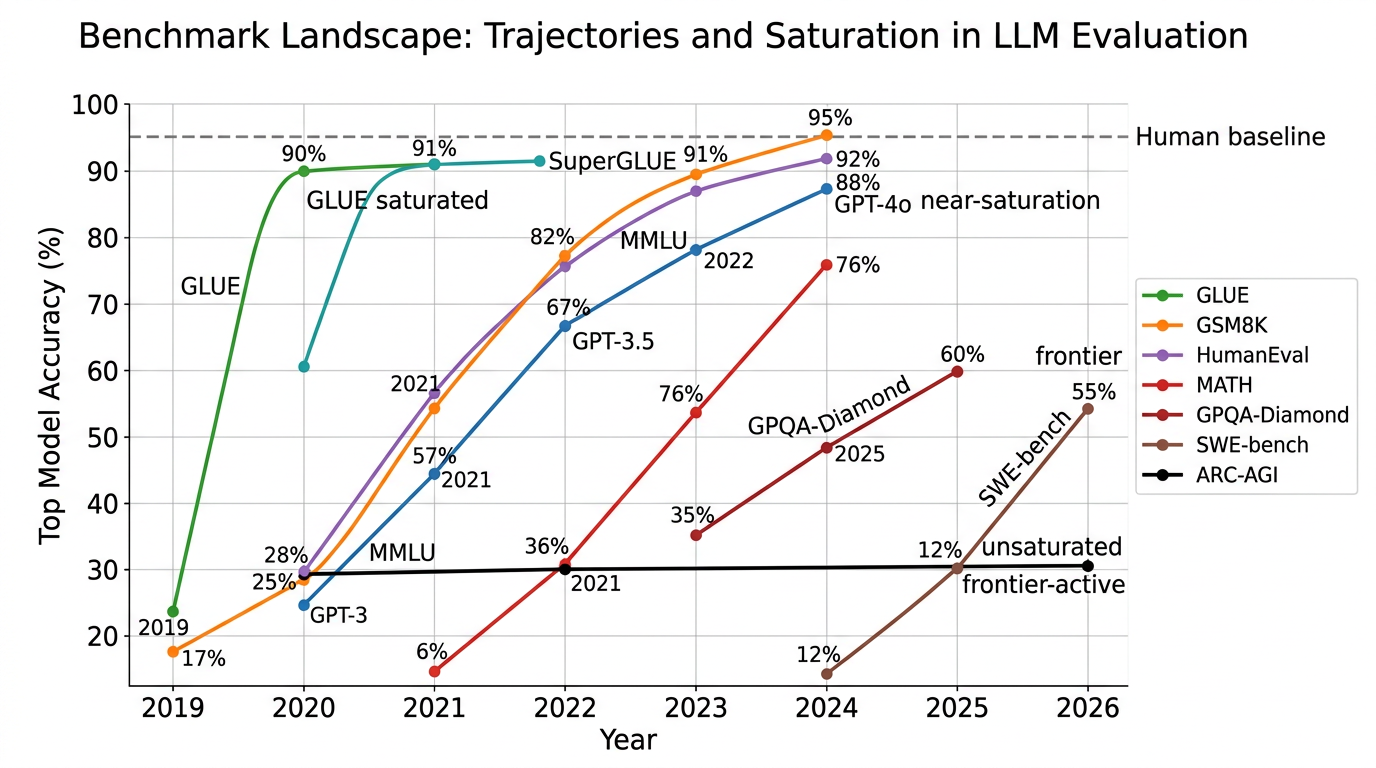
\includegraphics[width=\linewidth,keepaspectratio]{./figures/Evaluation-of-Large-Language-Models__fig4_landscape.png}}
\caption{Benchmark Landscape: Trajectories and Saturation}\label{fig:fig4-landscape}\end{figure}

\subsection{Major Evaluation Frameworks: HELM, lm-evaluation-harness, Open LLM Leaderboard}\label{major-evaluation-frameworks-helm-lm-evaluation-harness-open-llm-leaderboard}

This subsection covers the major evaluation frameworks and their subleaderboards.

The Holistic Evaluation of Language Models (HELM) framework \cite{liang20222022,bommasani2023holisticevaluation} is the most extensive single evaluation infrastructure. HELM v1 reported 30 models across 16 core scenarios with seven metrics --- accuracy, calibration, robustness, fairness, bias, toxicity, efficiency. HELM v2 added the HELM Lite, HELM Capability, HELM Safety, HELM Instruct, HELM MMLU, HELM Air-Bench, HELM Code, HELM Heim, and HELM Math subleaderboards by 2024. Each subleaderboard runs a precise scenario × metric grid; HELM Capability covers MMLU, GPQA, MATH, GSM8K, IFEval, BBH, and others; HELM Safety covers the bias, toxicity, and harm panels. HELM publishes a manifest of prompts, target answers, and expected metric outputs for each scenario, enabling reproduction by third parties. As of 2025, HELM had evaluated 200+ open and closed models across thousands of scenario-metric cells.

The EleutherAI \textbf{lm-evaluation-harness} \cite{biderman20242024} is the most widely adopted open-source evaluation library. The harness provides a standardised task interface, supports both log-likelihood-based and free-generation evaluation, and includes pre-implemented adapters for hundreds of benchmarks: ARC, HellaSwag, MMLU, TruthfulQA, WinoGrande, GSM8K, MATH, MBPP, HumanEval, BBH, AGIEval, BBQ, BLiMP, GLUE, SuperGLUE, BIG-Bench, MMLU-Pro, MMLU-CF, MGSM, IFEval, MUSR, GPQA, and more. The harness enforces deterministic prompt templates, fixed in-context exemplars, and reproducible random seeds. Lessons from the Trenches \cite{biderman20242024} documents systematic challenges: log-likelihood vs free-generation answer extraction can shift MMLU scores by 3-7 points; the choice of in-context exemplars can shift GSM8K by 5-10 points; subtle tokenizer differences (BPE vs SentencePiece) can shift HumanEval pass@1 by 1-3 points.

The \textbf{HuggingFace Open LLM Leaderboard} v1 evaluated open-weights models on six benchmarks via the lm-evaluation-harness: ARC-Challenge, HellaSwag, MMLU, TruthfulQA, WinoGrande, and GSM8K. Saturation prompted Open LLM Leaderboard v2 (June 2024), which replaces the saturated stack with IFEval (instruction-following), BBH (reasoning), MATH-Hard (level 5 only), GPQA, MUSR (multi-step reasoning), and MMLU-Pro. The v2 average is 50\% lower than v1 for many top models, restoring discrimination among frontier checkpoints.

\textbf{OpenAI Evals} is a permissive registry-based framework for community-contributed evaluations, used both internally for GPT-4 release evaluation and externally by third parties. \textbf{BIG-Bench} ships its own evaluation harness with 204 task implementations. \textbf{vLLM-Bench} and \textbf{AlpacaEval} provide additional infrastructure. \textbf{MTEB} (Massive Text Embedding Benchmark) covers embedding models. \textbf{Big-Bench Hard} ships a separate runnable harness used in many follow-up papers including Suzgun et al.'s CoT analysis \cite{suzgun2022challengingbigbenc}. The Hugging Face Lighteval and Vellum offer alternative entry points; the Stanford CRFM HELM CLI provides a unified CLI for HELM.

A separate frontier-model layer is the \emph{live arena infrastructure}: LMSYS Chatbot Arena \cite{chiang20242024} uses a fastchat backend serving anonymised models behind a battle interface, with vote storage in PostgreSQL and Elo computation by bootstrap; Arena-Hard \cite{li20242024} uses the BenchBuilder pipeline to curate prompts; SWE-Bench-Live spins up Docker containers per-issue; GAIA exposes web-browsing and code-execution tools through an evaluation harness. All four are infrastructure-heavy and require substantial cloud resources.

\subsection{Compute and Cost Profiling Across Benchmarks}\label{compute-and-cost-profiling-across-benchmarks}

This subsection profiles representative compute and dollar costs for each major benchmark.

Evaluation compute and cost scale with model size, benchmark size, sample count, and judge usage. We profile representative costs below for a frontier 70B-class model evaluated on a single H100 GPU at 50 tokens/s, and for closed models accessed via API.

Order-of-magnitude figures across the canonical suites are as follows. MMLU 5-shot processes \textasciitilde4M tokens per model, costing \textasciitilde22 GPU-hours locally on a 70B model or \textasciitilde\$50 via API. GSM8K with CoT processes \textasciitilde5M tokens; self-consistency at 40 samples multiplies cost \textasciitilde40×. HumanEval pass@1 with 100 samples processes \textasciitilde3.3M tokens plus sandboxed test execution. BIG-Bench full processes \textasciitilde150-200M tokens, costing \textasciitilde$1,500-2,000 per API run. HELM Lite costs \textasciitilde$500-1,000 and HELM Capability \textasciitilde\$2,000-4,000 per model. MT-Bench needs \textasciitilde320 GPT-4 judge calls (\textasciitilde\$15-40), and Arena-Hard \textasciitilde2,000 judge calls (\textasciitilde\$30-80). SWE-bench Verified runs cost $50-300, full SWE-bench \textasciitilde5× higher, GAIA $10-100, and MLE-bench \$200-2,000 per agent. Chatbot Arena hosting costs LMSYS \$5,000-20,000 per month. RULER 128k can exceed \$5,000 per model under Claude 3 Opus pricing.

The HELM efficiency dimension reports tokens-per-second and dollar-cost-per-token alongside accuracy, surfacing cost-aware Pareto frontiers. The Open LLM Leaderboard does not currently report cost, drawing criticism that open-weights models are at a comparison disadvantage when both parameters and runtime are not normalised.

The Cost vs Capability summary table below illustrates the order-of-magnitude differences.

\begin{table*}[t]
\centering
\caption{Compute and Cost Profiling Across Benchmarks: comparative summary.}
\label{tab:compute-and-cost-profiling-across-benchmarks}
\begin{tabular}{>{\raggedright\arraybackslash}p{0.2687\linewidth}
  >{\raggedright\arraybackslash}p{0.1791\linewidth}
  >{\raggedright\arraybackslash}p{0.2090\linewidth}
  >{\raggedright\arraybackslash}p{0.1642\linewidth}
  >{\raggedright\arraybackslash}p{0.1791\linewidth}}
\toprule
Benchmark & Items & Tokens / model & Local (70B) & API (avg) \\
\midrule
MMLU 5-shot & 15,908 & \textasciitilde4M & \textasciitilde22 GPU-h & \textasciitilde\$50 \\
MMLU-Pro & 12,032 & \textasciitilde4M & \textasciitilde22 GPU-h & \textasciitilde\$50 \\
GSM8K (CoT) & 1,319 & \textasciitilde5M & \textasciitilde28 GPU-h & \textasciitilde\$60 \\
GSM8K (CoT + SC) & 1,319 & \textasciitilde200M & days & \textasciitilde\$2,000 \\
MATH (CoT) & 12,500 & \textasciitilde30M & days & \textasciitilde\$300 \\
HumanEval (k=100) & 164 & \textasciitilde3M & \textasciitilde16 GPU-h & \textasciitilde\$30 \\
BIG-Bench full & 204 tasks & \textasciitilde150-200M & days & \textasciitilde\$2,000 \\
BBH & 23 tasks & \textasciitilde12M & \textasciitilde70 GPU-h & \textasciitilde\$120 \\
HELM Lite & 10 scenarios & \textasciitilde80M & days & \textasciitilde\$800 \\
HELM Capability & 30 scenarios & \textasciitilde300M & week & \textasciitilde\$3,000 \\
MT-Bench (judge) & 80 & small + judge & \textless1 GPU-h & \textasciitilde\$25 \\
Arena-Hard & 500 & small + judge & small & \textasciitilde\$50 \\
SWE-bench Verified & 500 & \textasciitilde150M & days & \textasciitilde\$200 \\
GAIA & 466 & \textasciitilde25M & hours & \textasciitilde\$50 \\
MLE-bench & 75 comps & very large & days-weeks & \textasciitilde\$1,500 \\
RULER 128k & 1,300 long & \textasciitilde200M & days & \textasciitilde\$5,000 \\
Chatbot Arena & continuous & n/a & n/a & \$10k+/month \\
\end{tabular}
\end{table*}

\subsection{Reproducibility, Decoding Settings, and Prompt Sensitivity}\label{reproducibility-decoding-settings-and-prompt-sensitivity}

This subsection enumerates the seven reproducibility levers that drive cross-paper score variance.

A persistent challenge in LLM evaluation is the reproducibility of reported numbers. Lessons from the Trenches \cite{biderman20242024} documents that the same model can produce different MMLU scores across the lm-evaluation-harness, OpenAI Evals, HELM, and BIG-Bench harness due to differences in answer extraction, prompt templates, in-context exemplars, decoding temperature, batched-inference numerical effects, and tokenization. The MMLU-CF paper \cite{zhao20242024} notes 5-15 percentage-point spreads on the same model across these frameworks.

The most consequential reproducibility levers are:

\begin{enumerate}
\def\labelenumi{\arabic{enumi}.}

\item
  \textbf{Answer extraction}: log-likelihood comparison (used by lm-eval-harness for MCQ) versus free generation + regex extraction (used by HELM and the original MMLU paper). A model that struggles to follow the ``Answer: X'' format will be penalised under free generation but not log-likelihood.
\item
  \textbf{Decoding temperature}: 0.0 (greedy) versus 0.7-0.8 (sampling) versus 0.6 with top-p 0.95. Math benchmarks with self-consistency require sampling; pass@k requires sampling.
\item
  \textbf{In-context exemplar choice}: order, content, and number of exemplars shift scores. Studies have shown 5-10\% spreads on GSM8K across exemplar permutations.
\item
  \textbf{Tokenizer}: BPE versus SentencePiece versus tiktoken. The Tokenizer Unfairness paper \cite{petrov20232023} documents 2-7× length differences for non-Latin scripts.
\item
  \textbf{System prompts and chat templates}: Llama-3 chat versus base templates differ in performance by 3-8 points on instruction-following tasks; Tools/JSON-schema prompts shift code benchmark scores.
\item
  \textbf{Batched-inference effects}: numerical non-determinism in attention can shift scores by 0.1-0.3 points on identical inputs across hardware.
\item
  \textbf{Time-of-evaluation}: closed-model APIs may be retrained between releases, so a ``GPT-4'' score reported in March 2023 differs from one in March 2024.
\end{enumerate}

Mitigations include the harness publishing exact prompt templates and seed lists; HELM publishing the full output trace per item; OpenAI Evals storing the model snapshot identifier in each result; and the AI Benchmark Half-Life \cite{white20242024} proposing time-stamped benchmark releases. The CONDA shared task \cite{sainz20242024} standardised contamination-detection protocols.

Two reproducibility incidents illustrate the stakes. The GPT-4 MMLU controversy showed a 1-2 point gap between OpenAI's 86.4\% {[}OpenAI, 2023{]} under custom free-generation extraction and community runs at 84.7-85.5\% under default 5-shot log-likelihood. The SWE-bench leaderboard inflation issue showed that adversarial test-suite mutations reduce reported Verified scores by 10-20 points \cite{yu20262026}, motivating SWE-rebench's date-stamped decontamination \cite{badertdinov20252025}. Reproducibility infrastructure now ships with JSON manifests covering model snapshot, decoding parameters, prompt template, in-context exemplars, harness version, seed list, and expected output traces.

For a practitioner releasing a new LLM, the recommended evaluation manifest in 2026 contains: (i) MMLU and MMLU-Pro under both 0-shot and 5-shot with both log-likelihood and free-generation extraction; (ii) GSM8K, MATH, MBPP, HumanEval with greedy decoding and one self-consistency variant; (iii) BBH 3-shot CoT; (iv) IFEval and AlpacaEval 2 LC; (v) MT-Bench score with GPT-4 judge; (vi) GPQA-Diamond with greedy and majority-vote-of-32; (vii) HELM Lite or Capability core panel; (viii) RULER at the deployment context length; (ix) BBQ and TruthfulQA for safety; (x) cost per benchmark and total wall-clock evaluation time. This recipe is approximated by the canonical model cards of LLaMA-3.1, Claude 3, Gemini 1.5, GPT-4o, and DeepSeek-R1 release reports.

The next section turns to the failure modes that make reproducible evaluation hard: data contamination, prompt sensitivity, and benchmark saturation under Goodhart's law.

\section{Failure Modes, Contamination, and Methodological Pitfalls}\label{failure-modes-contamination-and-methodological-pitfalls}

Whereas Section 10 covered the infrastructure that makes evaluation reproducible, this section catalogues the failure modes that erode validity even when infrastructure is correctly used. This section reviews three failure clusters: data contamination (Section 11.1), prompt and tokenizer sensitivity (Section 11.2), and saturation under Goodhart's law (Section 11.3), followed by a synthesis subsection. Representative methods include: GSM1k (Zhang 2024, 1,250 contamination probes), MMLU-CF (Zhao 2024, 8,000 leakage-screened items), MMLU-Pro (Wang 2024, harder distractors), Min-K\%-Prob (Shi 2024, low-probability-token detection), CDD (Sela 2026, output-distribution contamination detection), n-gram overlap detection (CONDA Sainz 2024), perplexity-gap detection, MIA (membership inference attacks), adversarial-compression detection \citep{schwarzschild20242024}, Carlini memorisation probes (2023), Dynamic-KGQA (Dammu 2025, KG-generated items), DynaCode (Hu 2025, controlled cyclomatic complexity), Jailbreak Distillation (Zhang 2025, renewable safety probes), SWE-rebench (Badertdinov 2025, decontaminated SWE-bench), SWE-ABS (Yu 2026, adversarial mutations), RADAR (Kattamuri 2025, mechanistic-pathway analysis), PromptBench (10 attack types), PPTC-R (Zhang 2024, PowerPoint robustness), and the AI Benchmark Half-Life framework \citep{white20242024}.

The growing body of LLM evaluation literature has been accompanied by an equally rapid catalogue of failure modes: data contamination \cite{sainz20242024}, prompt sensitivity \cite{biderman20242024}, saturation and Goodhart-style benchmark erosion \cite{white20242024}, judge biases \cite{gu20242024}, and construct-validity gaps in safety probes \cite{yang20242024}. This section synthesises the failure-mode literature into a single map and documents the mitigations that have entered standard practice.

\subsection{Data Contamination, Memorization, and the GSM1k Result}\label{data-contamination-memorization-and-the-gsm1k-result}

This subsection covers the three contamination phenomena and the GSM1k empirical demonstration.

Data contamination occurs when test items leak into a model's training corpus, inflating reported scores without genuine generalisation. Three distinct phenomena are captured under this umbrella. \textbf{Input contamination} occurs when the test prompt appears verbatim in pre-training, allowing token-level memorisation. \textbf{Label contamination} occurs when the (input, gold output) pair appears, allowing exact answer recall. \textbf{Order contamination} occurs when the test split is included in the training data with the same item ordering, allowing a model to exploit dataset structure.

Carlini et al.~(2023) showed that LLMs memorise sufficiently common training data, with memorisation rising under model scale and training duration. The CONDA shared task \cite{sainz20242024} aggregated 60+ contamination-detection submissions in 2024. The Taxonomy for Data Contamination \cite{palavalli2024ataxonomyfordataco} formalised the three phenomena above. Detection methods surveyed by Fu et al.~{[}2025{]} include 13-gram overlap, perplexity gap, Min-K\%-Prob, CDD output-distribution detection \cite{sela2026nomemorizationnode}, and adversarial compression \cite{schwarzschild20242024}.

The most striking empirical demonstration of contamination effects came from Zhang et al.'s GSM1k \cite{zhang20242024}, who hand-authored 1,250 new arithmetic problems matching the GSM8K distribution and observed that several open-weight models scored 8-13 percentage points lower on GSM1k than on GSM8K, while frontier closed models retained their score. The same pattern repeats across MMLU (a widely-leaked benchmark) and HumanEval (where 18\% of problems show overlap with training data per Quantifying Contamination \cite{riddell2024quantifyingcontami}).

Contamination-aware benchmarks include MMLU-CF \cite{zhao20242024} (8,000 items after leakage screening), MMLU-Pro \cite{wang20242024} (harder distractors and increased option count), Dynamic-KGQA \cite{dammu2025dynamickgqaascalab} (synthetic generation from knowledge graphs), Jailbreak Distillation \cite{zhang20252025} (renewable safety probes), and SWE-rebench \cite{badertdinov20252025} (decontaminated SWE-bench). The AI Benchmark Half-Life paper \cite{white20242024} estimates that a popular benchmark's validity decays exponentially with a half-life of 12-18 months under uncontrolled re-training.

Live evaluation defeats contamination by construction. Chatbot Arena's prompts arrive after the training cutoff. SWE-Bench-Live, MLE-bench, and GAIA require interaction with up-to-date web data and tool-execution traces. RADAR \cite{kattamuri20252025} proposes mechanistic pathways for contamination detection. None of the Others {[}Sánchez Salido et al., 2025{]} introduces a general technique for distinguishing reasoning from memorisation in MCQ benchmarks.

A subtler mode of contamination is \textbf{alignment-by-evaluation}: when a model is fine-tuned on data labelled by GPT-4, then evaluated by GPT-4 as judge, performance is artificially inflated \cite{wei20242024}. Mitigations include rotating judges, using open-judge models (Prometheus 2, JudgeLM), and reporting human-judge agreement on a held-out subset.

\subsection{Prompt Sensitivity, Few-Shot Order Effects, and Tokenizer Bias}\label{prompt-sensitivity-few-shot-order-effects-and-tokenizer-bias}

This subsection covers the four pernicious sources of variance that shift scores in ways that should be incidental.

The second cluster of failure modes concerns \emph{non-robustness} to evaluation choices that should be incidental. Lessons from the Trenches \cite{biderman20242024} documents four pernicious sources of variance.

\textbf{Few-shot exemplar order} shifts MMLU scores by 1-3 points and GSM8K scores by 5-10. The lm-evaluation-harness pins a fixed seed and exemplar list. \textbf{Prompt template phrasing} can shift MMLU by 1-4 points when ``Question:'' becomes ``Q:'' or the ``Answer:'' cue is removed. PromptBench perturbs prompts along character, word, sentence, and semantic dimensions; PPTC-R \cite{zhang20242024} does the same for PowerPoint tasks. \textbf{Tokenizer choice} matters: LLaMA's BPE splits ``ChatGPT'' into 3 tokens, GPT-4's \(cl100k_b\)ase into 1, and non-Latin scripts cost 2-7× more tokens \cite{petrov20232023}. \textbf{Decoding non-determinism} flips the greedy token in 0.1-0.5\% of items because batched-inference kernels introduce 1e-6 numerical jitter, mitigated by deterministic cuDNN flags and FlashAttention pins.

Two further issues are noteworthy. Instruction-template mismatch shifts MT-Bench scores by 1-3 points when a base LLM is run with a chat template or vice-versa. Prompt-injection robustness matters whenever retrieval is allowed: malicious content in the retrieved corpus can alter answers, as documented for translation \cite{sun2024scalingbehaviorofm}.

\subsection{Saturation, Goodhart's Law, and Benchmark Half-Lives}\label{saturation-goodharts-law-and-benchmark-half-lives}

This subsection covers benchmark saturation, validity decay, and Goodhart-style optimisation pressure.

The third failure-mode cluster concerns \textbf{benchmark saturation}: once accuracy approaches the ceiling, the benchmark loses discriminative power. GLUE saturated within two years of release; SuperGLUE within three; MMLU within four; HumanEval within four; HellaSwag, ARC-Easy, WinoGrande, and BoolQ are all saturated as of 2025. The AI Benchmark Half-Life paper \cite{white20242024} proposes a theory of validity decay: in a regime of recursive corpora, a benchmark's discriminative validity decays as \(V(t) = V_0 \exp(-\lambda t)\) with \(\lambda \approx 1/(12-18 \text{ months})\) for popular suites. The paper recommends time-stamped releases with cryptographic commitments.

Goodhart's law manifests through four patterns: training data curated to oversample benchmark-similar examples, evaluation prompts reverse-engineered to maximise scores (SWE-bench test-targeting \cite{yu20262026}), architectures and objectives tuned to specific benchmarks (math-specific RLHF for AIME and GSM8K), and judge gaming via stylistic conformance to GPT-4 preferences. Mitigations include frequent benchmark refresh (Open LLM Leaderboard v2, MMLU-Pro, BBEH, GPQA, FrontierMath, HLE), live arenas (Chatbot Arena, Arena-Hard, SWE-Bench-Live), benchmark mutations (SWE-ABS, Saving SWE-Bench \cite{garg2025savingswebenchaben}), cost-aware leaderboards \cite{kapoor20242024}, and process-level evaluation.

\subsection{Failure-mode synthesis}\label{failure-mode-synthesis}

The table below summarises the major failure modes, their typical magnitude, and the standard mitigations.

\begin{table*}[t]
\centering
\caption{Failure-mode synthesis: comparative summary.}
\label{tab:failure-mode-synthesis}
\begin{tabular}{>{\raggedright\arraybackslash}p{0.2308\linewidth}
  >{\raggedright\arraybackslash}p{0.2098\linewidth}
  >{\raggedright\arraybackslash}p{0.1678\linewidth}
  >{\raggedright\arraybackslash}p{0.3916\linewidth}}
\toprule
Failure mode & Magnitude & Affected benchmarks & Mitigation \\
\midrule
Test data leakage (input) & 0-10 pts inflation & MMLU, GSM8K, HumanEval & Decontamination filters (MMLU-CF, MMLU-Pro), live arenas \\
Test data leakage (label) & 5-20 pts inflation & older static benchmarks & New benchmarks, GSM1k probes \\
Memorisation & 5-15 pts inflation & trivia, factual QA & Min-K\%-Prob, n-gram detection, dynamic generation \\
Few-shot exemplar order & 1-10 pts variance & MMLU, GSM8K & Fixed seed, fixed exemplar list, lm-eval-harness \\
Prompt template phrasing & 1-5 pts variance & most & Standardised templates, HELM manifest \\
Tokenizer length bias & 2-7× length non-Latin & multilingual & BPE-aware fairness, dedicated multilingual evals \\
Chat-template mismatch & 1-3 pts & instruction-following & Apply official chat template \\
Batched-inference non-determinism & 0.1-0.5 pts & all greedy decoding & Deterministic kernels, multi-seed aggregation \\
Judge bias (position) & 1-5 pts & MT-Bench, AlpacaEval & Position swapping \\
Judge bias (length) & 5-15 pts & AlpacaEval & Length-controlled win-rate \\
Judge bias (self-preference) & 2-8 pts & LLM-as-Judge & Multi-judge ensembling, open judges \\
Saturation & gradual loss of discrimination & GLUE → MMLU → HumanEval & Refresh (MMLU-Pro, BBEH, GPQA, HLE) \\
Goodhart targeting & undisclosed & targeted benchmarks & Live arenas, blind eval, mutation tests \\
Test-targeting on SWE-bench & 10-20 pts inflation & SWE-bench Verified & SWE-ABS mutations, decontamination \\
Bias-benchmark refusal & unclear & BBQ, RealToxicityPrompts & Pair with capability scores \\
Prompt injection in retrieval & varies & RAG benchmarks & Sanitisation, attack-aware evaluation \\
Construct validity gap (causal) & unmeasured & causal-reasoning suites & Refined benchmarks \citep{yang20242024} \\
Multi-turn safety drift & 15-40 pts & single-turn safety & MTSA multi-round testing \\
Live-arena vote rigging & 5-10 pts in Elo & Chatbot Arena & Anti-fraud aggregation, fingerprinting \\
\end{tabular}
\end{table*}

Four observations emerge from this catalogue. First, no single benchmark is robust to all failure modes simultaneously. Robust evaluation requires triangulation across multiple benchmarks (MMLU + MMLU-Pro + GPQA), multiple methodologies (static + live + judge-based), and multiple seeds. Second, construct validity remains weak: TruthfulQA measures imitative-falsehood resistance, BBQ measures stereotype-aligned preference, and HumanEval measures isolated synthesis, none of which fully spans the parent construct. Third, evaluation cost is rising: a SWE-bench Verified run costs \$200-500, a HELM Capability run \$3,000-6,000, and an MLE-bench run \$2,000+. Fourth, evaluation has become a compliance instrument under the EU AI Act, NIST AI Risk Management Framework, and US Executive Order 14110.

Crucially, the pattern points to one conclusion: evaluation must itself be evaluated. Each new benchmark needs a contamination probe, a robustness ablation, a discrimination analysis, a cost report, and a construct-validity argument \cite{biderman20242024,yang20242024}. Section 12 turns to open problems and predictions for the next phase.

\section{Open Problems and Forecasts for 2026 and Beyond}\label{open-problems-and-forecasts-for-2026-and-beyond}

Building on the failure-mode catalogue in Section 11, this section identifies the open research problems that will define LLM evaluation through 2030 and offers falsifiable forecasts for how the field will respond. The evaluation of large language models has matured rapidly, but several structural problems remain unsolved. This section catalogues the main open problems and offers falsifiable predictions for the next 3-5 years. The map of open problems is illustrated in Figure 5.

\subsection{Critical Synthesis: Comparing the Major Method Families}\label{critical-synthesis-comparing-the-major-method-families}

Before listing open problems, it is useful to compare the major evaluation method families that recur across the survey. PPO-style RLHF \cite{ouyang20222022} trades off explicit reward-model fitting and KL regularisation against sample efficiency, while DPO \cite{rafailov2023directpreferenceop} optimises the implicit-reward closed form directly from preference pairs and avoids reward-model drift, and GRPO (DeepSeek-R1, 2025) replaces value baselines with group-relative reward normalisation to scale to long reasoning chains. Reference-based metrics (BLEU, ROUGE, BERTScore) trade reproducibility for low correlation with human preference, while judge-based metrics (G-Eval, MT-Bench, Arena-Hard) trade API dependence for high Elo correlation, and human pairwise (Chatbot Arena) gives ground truth at the cost of irreproducibility. Static splits (MMLU, GSM8K, HumanEval) trade contamination resistance for reproducibility, while live arenas (Chatbot Arena, SWE-Bench-Live) trade reproducibility for contamination resistance, and dynamic generation (Dynamic-KGQA, DynaCode, JBDistill) attempts to bridge both at the cost of naturalness. Outcome-only metrics (exact-match) trade interpretability for cost, while process reward models (PRMs trained on PRM800K) trade annotation cost for trace-level diagnostic power. Across these families, no single method dominates and triangulation across multiple paradigms remains the empirical state of the art.

The eight specific open problems that structure the rest of this section are:

\begin{itemize}

\item
  Process-level and reasoning-trace evaluation (Section 12.1).
\item
  Decontamination-by-design and time-stamped live benchmarks (Section 12.2).
\item
  Standardisation of agent evaluation and cost-aware leaderboards (Section 12.3).
\item
  Multilingual fairness and parity across 50+ languages.
\item
  Joint safety-capability Pareto reporting.
\item
  Meta-evaluation: judge agreement, prompt robustness, contamination probes.
\item
  Calibration and uncertainty quantification on release cards.
\item
  Human-AI team-level evaluation and agentic safety.
\end{itemize}

The five future directions that we forecast will emerge in 2026-2027 are:

\begin{itemize}

\item
  Process reward models scoring intermediate reasoning steps as standard release-card items.
\item
  Live arenas (Chatbot Arena, Arena-Hard, SWE-Bench-Live) replacing saturated static splits as the primary instruction-following ranking.
\item
  Cost-aware Pareto leaderboards (HELM Cost, AI Agents That Matter) replacing single-scalar leaderboard ranks.
\item
  Multimodal HELM panels covering text, vision, audio, and video under a unified harness.
\item
  Verbatim-extraction and membership-inference probes on release cards alongside contamination probes.
\end{itemize}

\begin{figure}[t]
\centering
\pandocbounded{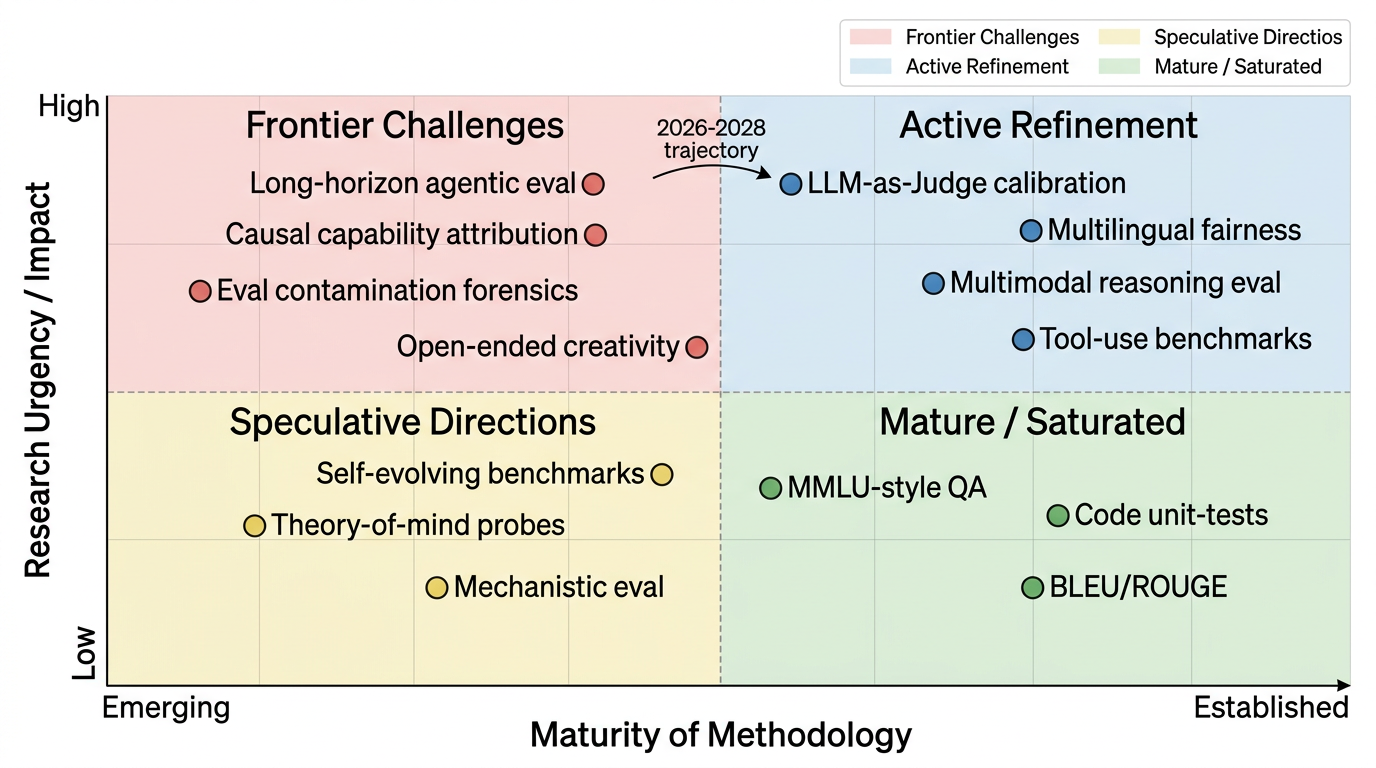
\includegraphics[width=\linewidth,keepaspectratio]{./figures/Evaluation-of-Large-Language-Models__fig5_openmap.png}}
\caption{Open Problems and Forecasts in LLM Evaluation}\label{fig:fig5-openmap}\end{figure}

\subsection{Process-Level and Reasoning-Trace Evaluation}\label{process-level-and-reasoning-trace-evaluation}

This subsection covers process-reward models and trace-consistency evaluation as alternatives to outcome-only scoring.

The first open problem concerns the evaluation of reasoning \emph{processes}, not only outcomes. Reasoning-trained models such as OpenAI o1 (released September 2024), DeepSeek-R1 {[}DeepSeek-AI, 2025{]}, Gemini 2.0 Thinking, and the Towards Reasoning Era models surveyed by Chen et al.~\cite{chen20252025} generate 5,000-50,000-token chains of thought before producing a final answer. Outcome-only metrics (exact-match on AIME, GSM8K) cannot distinguish a model that reaches the right answer through correct reasoning from one that gets there via a hallucinated intermediate step that happens to land on the gold answer.

Process Reward Models (PRMs) trained on step-level annotations have emerged as the leading direction. The PRM800K dataset \citep{lightman20242024} supplies 800k step-level human labels (correct, incorrect, neutral) on MATH solutions. PRM-based scoring is used by OpenAI o1's Best-of-N decoding and by DeepSeek-R1 evaluation. Towards Large Reasoning Models \cite{xu20252025} surveys the rapidly expanding space. Towards Reasoning Era \cite{chen20252025} catalogues long-CoT evaluation methods. SWE-Shepherd \cite{dihan2026sweshepherdadvanci} proposes PRMs for code agents.

A complementary direction is \textbf{trace consistency} evaluation: does the chain of thought arrive at conclusions consistent with its premises? FinChain \cite{xie20252025} verifies symbolic financial reasoning chains. LongCoT \cite{motwani20262026} benchmarks long-horizon planning. DiffCoT \cite{cao20262026} explores diffusion-style reasoning chains. We forecast that by 2027, frontier-model release cards will report \emph{trace-consistency scores} alongside answer accuracy.

A third direction is \textbf{meta-reasoning} evaluation: MR-GSM8K {[}Zeng et al., 2023{]} flips the role of the model from solver to grader, requiring it to score student solutions. Meta-reasoning probes the depth of mathematical understanding more directly than answer-level metrics.

\subsection{Decontamination-by-Design and Time-Stamped Live Benchmarks}\label{decontamination-by-design-and-time-stamped-live-benchmarks}

This subsection covers the three decontamination strategy families: time-stamped live benchmarks, encrypted gold labels, and synthetic generation.

The second open problem is contamination resistance. As we documented in Section 11, popular static benchmarks have a half-life of 12-18 months under recursive corpus growth \cite{white20242024}. Three families of decontamination strategies are emerging.

\textbf{Time-stamped live benchmarks}: SWE-Bench-Live, Arena-Hard, BenchBuilder \cite{li20242024}, and SWE-rebench \cite{badertdinov20252025} curate prompts after model training cutoffs. The Chatbot Arena protocol \cite{chiang20242024} is the canonical example: 10 million+ battles by 2026 with a continuously updating Elo. We forecast that by 2027, every major model release will report a live-arena Elo alongside static benchmarks.

\textbf{Encrypted gold labels}: a benchmark publishes inputs but withholds gold answers; evaluation is performed via a remote API. The HELM Capability private subset implements partial encryption. We forecast that contamination-resistant benchmarks for high-stakes domains (medicine, law, defence) will increasingly use encrypted-gold-label protocols.

\textbf{Synthetic and dynamic generation}: Dynamic-KGQA \cite{dammu2025dynamickgqaascalab}, DynaCode \cite{hu20252025}, JBDistill \cite{zhang20252025} generate fresh items from templates and seeds. The trade-off is reduced naturalness; the gain is renewability. We forecast hybrid synthetic-natural benchmarks will become standard, with synthetic items used as decontamination sentinels.

A specific open problem is \textbf{detection of order contamination}: items appearing in the test set with the same ordering as in pre-training. Current detection methods focus on input-pair contamination; ordering effects are under-studied. RADAR \cite{kattamuri20252025} proposes mechanistic-pathway analysis but is in early stages.

\subsection{Standardizing Agent Evaluation and Cost-Aware Leaderboards}\label{standardizing-agent-evaluation-and-cost-aware-leaderboards}

This subsection covers the standardisation gap in agent evaluation and the emerging cost-aware leaderboard regime.

The third open problem is the heterogeneity of agent evaluation. Yehudai et al.~\cite{yehudai20252025} and Mohammadi et al.~\cite{mohammadi20252025} surveys document 50+ agent benchmarks with incompatible scoring protocols, environment configurations, and tool stacks. AI Agents That Matter \cite{kapoor20242024} argues that current agent leaderboards are cost-blind and proposes Pareto frontiers of accuracy versus cost.

The open problems within agent evaluation include: (i) standardisation of environment APIs (browser, code interpreter, OS), (ii) reproducibility of multi-step traces, (iii) sandboxing for security and safety, (iv) trajectory-level diagnostics (failure-mode classification along the action graph). The Mind the Gap paper \cite{wicaksono20252025} proposes action-graph observability for agent red-teaming. SWE-Debate \cite{li20252025} explores multi-agent debate.

A specific forecast: by 2027 we expect a unified \textbf{AgentBench-2} standard that prescribes a fixed environment manifest, a deterministic tool API, and a cost-aware reporting format. The current SWE-bench Verified, GAIA, MLE-bench, and OSWorld are likely candidates for unification.

A second forecast: cost-aware leaderboards will become standard. The HELM Capability Cost panel and the Open LLM Leaderboard's emerging cost reports already point in this direction. The expected reporting unit is \emph{per-task cost in USD} alongside \emph{accuracy}.

\subsection{Additional open problems}\label{additional-open-problems}

\textbf{Multilingual fairness}: the gap between English MMLU (90\%+) and low-resource MMLU (50-65\%) for Bengali, Yoruba, and Burmese remains large. The MEGA \cite{ahuja20232023} and SEA-HELM \cite{susanto20252025} efforts pushed coverage but parity is far. Forecast: by 2030, frontier-model release cards will include parity scores across at least 50 languages.

\textbf{Safety-capability Pareto}: a model that refuses 90\% of inputs is safe but useless. The HELM Safety + Capability joint reporting partially addresses this. The Constitutional AI line \cite{bai20222022} explicitly trains for the joint objective. Forecast: standard release evaluations will report a \emph{helpfulness-harmlessness Pareto} with at least three operating points.

\textbf{Evaluation of evaluation}: as judges (GPT-4) and benchmarks (MMLU) themselves evolve, evaluation becomes a moving target. The Personalized Judges paper \cite{dong2024canllmbeapersonali}, the Vote Rigging paper \cite{min20252025}, and the Critical Review of Causal Reasoning Benchmarks \cite{yang20242024} argue for meta-evaluation as a research priority. Forecast: by 2027, evaluation papers will routinely include a meta-evaluation section reporting judge-agreement, prompt-robustness, and contamination-probe results.

\textbf{Reasoning generalisation}: tests of out-of-distribution reasoning (ARC-AGI, HumanityLastExam, FrontierMath) reveal that frontier models still struggle with novel structures. ARC-AGI 2 (2024) and ARC-AGI 3 (announced 2025) are designed to remain hard; humans solve 85\%+, frontier models \textless15\%. Forecast: ARC-AGI-style novel-task benchmarks will become a standard frontier-evaluation panel by 2027.

\textbf{Calibration and uncertainty}: hallucination rates remain high (5-30\% on long-form factuality), and frontier models are systematically over-confident. SimpleQA \cite{wei20242024} explicitly measures hallucination rate; HELM measures calibration ECE (Expected Calibration Error). Forecast: well-calibrated uncertainty estimates will become a release-card requirement.

\textbf{Agentic safety}: as agents act on the web, file systems, and databases, the boundary of safety evaluation expands. Mind the Gap \cite{wicaksono20252025}, MTSA multi-turn safety \cite{guo20252025}, BlueSuffix RL defence \cite{zhao20242024}, and Latent Adversarial Training \cite{sheshadri20242024} open this space. Forecast: agentic safety benchmarks will dominate 2027-2028 safety-evaluation work.

\textbf{Human-AI collaboration evaluation}: where the LLM is one node in a human-AI workflow, individual model scores are insufficient. Recent work on personal-health agents \cite{merrill20262026} and clinical-decision agents \cite{schmidgall20262026} exemplifies this. Forecast: emerging composite benchmarks will measure team-level performance with human-in-the-loop.

\textbf{Privacy and memorisation}: extracting verbatim training data via membership inference attacks (MIA) is a privacy concern. CDD \cite{sela2026nomemorizationnode} and adversarial-compression \cite{schwarzschild20242024} propose detection. Forecast: by 2027, model release reports will include verbatim-extraction probes alongside contamination probes.

\textbf{Cross-modal evaluation}: vision-language, audio-language, and video-language models require unified evaluation. MME \cite{fu20232023}, LVLM-eHub \cite{xu20232023}, and Towards Holistic Evaluation of LALMs \cite{yang20252025} are early efforts. UniEval \cite{li20252025} proposes unified multimodal evaluation. Forecast: a HELM-Multimodal panel covering vision, audio, video, and text under one harness.

The summary table below condenses the open-problem agenda.

\begin{table*}[t]
\centering
\caption{Additional open problems: comparative summary.}
\label{tab:additional-open-problems}
\begin{tabular}{>{\raggedright\arraybackslash}p{0.2718\linewidth}
  >{\raggedright\arraybackslash}p{0.0680\linewidth}
  >{\raggedright\arraybackslash}p{0.3689\linewidth}
  >{\raggedright\arraybackslash}p{0.2913\linewidth}}
\toprule
Open problem & Year & Plausible benchmark response & Bottleneck \\
\midrule
Process-level reasoning eval & 2026-27 & PRM-based scoring, trace-consistency & Step-level annotation cost \\
Live decontaminated bench & 2026-28 & Arena-Hard 2, SWE-Bench-Live, MLE-Live & API access, hosting cost \\
Standardised agent eval & 2026-28 & AgentBench-2 unified spec & Environment heterogeneity \\
Cost-aware leaderboards & 2026-27 & HELM Cost, OpenLLM Cost & Closed-API pricing changes \\
Multilingual parity & 2027-30 & MEGA-2, SEA-HELM-2 & Annotation cost, low-res. data \\
Safety-capability Pareto & 2026-27 & Joint helpful-harmless eval & Annotation cost \\
Meta-evaluation & 2026-27 & Judge agreement metrics & Standardisation \\
ARC-AGI-style frontier & 2026-28 & ARC-AGI 3, novel-task benchmarks & Item authoring \\
Calibration / uncertainty & 2026-27 & ECE on release cards & Frontier-model probing access \\
Agentic safety & 2027-28 & Multi-turn agent red-team & Agent harness cost \\
Human-AI team eval & 2027-29 & Composite team benchmarks & Human-eval cost \\
Privacy / memorisation & 2026-28 & Verbatim extraction probes & Detection accuracy \\
Multimodal holistic & 2027-29 & HELM-Multimodal & Modality coverage \\
\end{tabular}
\end{table*}

Three meta-trends bind these forecasts. First, \textbf{the locus of evaluation is shifting from artefact (a static benchmark) to platform (a continually updated infrastructure)}. HELM, Chatbot Arena, Open LLM Leaderboard v2, and the SWE-bench-Live/Arena-Hard pipeline all instantiate this shift. Second, \textbf{evaluation cost is becoming a first-class constraint}: as frontier models grow more capable and chain-of-thought longer, naive evaluation budgets blow past \$10,000 per model run, motivating sample-efficient and judge-amortised protocols. Third, \textbf{safety, capability, and cost merge into a single Pareto report}: the future model release card will look more like a multi-metric dashboard than a single leaderboard rank.

We close this section with one cautionary forecast. As long as model training data is recursive --- i.e., as long as published benchmarks become training data for subsequent models --- there will be no permanently valid static benchmark. The half-life argument of White et al.~\cite{white20242024} makes this almost a theorem under uncontrolled scrape-based training corpora. The implication is that static benchmarks must be supplemented by, and increasingly subordinated to, live arenas and dynamic generation. The next decade of LLM evaluation will be defined by how well the field designs benchmarks that \textbf{stay hard} as models advance, while remaining \textbf{reproducible, cost-bounded, and safe} to administer at scale.

\section{Conclusion: Toward a Sustainable Evaluation Science for LLMs}\label{conclusion-toward-a-sustainable-evaluation-science-for-llms}

Building on Section 12's open-problem catalogue, this section consolidates the survey's central claims, articulates the persistent tensions in the field, and lists five concrete future directions that should guide LLM evaluation research through 2030.

This survey has mapped the evaluation of large language models from the BLEU and ROUGE metrics of 2002-2004 \cite{papineni2002bleuamethodforauto,lin2004rougeapackageforau}, through the GLUE/SuperGLUE classification era \cite{wang2018glueamultitaskbenc,wang2019superglueastickier}, the few-shot pivot of GPT-3 \cite{brown20202020}, the MMLU/BIG-Bench/HumanEval/GSM8K/TruthfulQA wave of 2021 \cite{hendrycks2021measuringmassivemu,chen20212021,cobbe20212021,lin2022truthfulqameasurin}, the Holistic Evaluation of Language Models \cite{liang20222022,bommasani2023holisticevaluation}, the LLM-as-a-Judge paradigm crystallised by MT-Bench and Chatbot Arena \cite{zheng20232023,chiang20242024}, the agent-evaluation explosion of GAIA, AgentBench, SWE-bench, and MLE-bench \cite{mialon2024gaiaabenchmarkforg,liu2023gevalnlgevaluation,jimenez20242024,chan20242024}, the contamination-aware MMLU-Pro/MMLU-CF/Arena-Hard family \cite{wang20242024,zhao20242024,li20242024}, the long-context RULER suite \cite{hsieh20242024}, and finally the frontier-knowledge GPQA-Diamond and Humanity's Last Exam benchmarks \cite{rein2024gpqaagraduatelevel,phan20252025} alongside the reasoning-trained DeepSeek-R1 and OpenAI o1 models {[}DeepSeek-AI, 2025{]}.

Three syntheses summarise the survey's central claims. First, the evaluation of LLMs has matured into an autonomous subfield with a stable conceptual scaffolding (the benchmark triple \((\mathcal{D}, \mathcal{M}, \mathcal{P})\), the seven HELM dimensions, the rule-based / embedding / judge / human metric stack), a coherent infrastructure layer (HELM, lm-evaluation-harness, Open LLM Leaderboard v2, OpenAI Evals, Chatbot Arena), and a recurring failure-mode catalogue (data contamination, prompt sensitivity, saturation, judge bias, construct-validity gap). The result is that an experienced practitioner can, in 2026, produce a defensible evaluation profile for a new model in a few days using off-the-shelf infrastructure --- a state of affairs that did not exist in 2020.

Second, no single benchmark is sufficient. The GPT-4 Technical Report {[}OpenAI, 2023{]}, the LLaMA-3.1 release card \cite{touvron20232023}, the Gemini 1.5 report {[}Gemini Team, 2024{]}, the Claude 3 family card, and the DeepSeek-R1 report {[}DeepSeek-AI, 2025{]} all combine 10-30 benchmarks across knowledge (MMLU 86-91\%, MMLU-Pro 71-84\%), reasoning (GSM8K 92-97\%, MATH 42-97\%, BBH 84-87\%, GPQA-Diamond 39-78\%, AIME 56-80\%), code (HumanEval 88-96\%, MBPP 80-86\%, SWE-bench Verified 25-70\%), dialogue (MT-Bench 7-9/10, Arena-Hard 50-79\%, Chatbot Arena Elo 1200-1290), safety (TruthfulQA MC2 50-84\%, HarmBench ASR varies), long-context (RULER 88\% at 32k), and multilingual (MGSM 79-92\%, C-Eval 80\%+). The recipe is now standard, even if its details continue to evolve.

Third, the field is shifting from outcome to process, from static to live, and from solo to agentic. Reasoning-trained models with 5,000-50,000-token chains of thought have made answer-only metrics insufficient; process reward models (PRMs) trained on PRM800K and similar datasets are now standard in frontier reasoning systems. Live arenas (Chatbot Arena, Arena-Hard, SWE-bench-Live) have made static splits obsolete for instruction-following measurement. Agentic benchmarks (GAIA, MLE-bench, OSWorld, OpenHands) have made single-turn QA insufficient for a complete capability picture. These shifts will accelerate through 2027.

Three persistent tensions remain. The first is \textbf{coverage versus depth}: holistic suites such as HELM cover dozens of scenarios but cannot probe each one to the depth of a specialist benchmark; specialist benchmarks lack breadth. Triangulation across multiple suites partially resolves this, but at significantly increased cost. The second tension is \textbf{contamination versus reproducibility}: live arenas combat contamination but defy reproduction; static splits reproduce but contaminate. Hybrid protocols (Arena-Hard, SWE-bench-Live, time-stamped MMLU-CF) attempt both. The third tension is \textbf{safety versus capability}: refusal-heavy alignment reduces harm potential but also reduces utility; the helpful-harmless Pareto remains an active research area. Constitutional AI \cite{bai20222022}, DPO \cite{rafailov2023directpreferenceop}, and the InstructGPT pipeline \cite{ouyang20222022} each try to push the frontier of this Pareto.

Looking forward, several anchoring numerical predictions can be made. By 2027, frontier-model MMLU saturation will reach 95\%+ (already at 92\% in 2025), forcing reliance on MMLU-Pro and GPQA-Diamond as primary knowledge tests. By 2027, frontier-model GSM8K and MATH will be functionally saturated near 100\%, forcing reliance on AIME, FrontierMath, and Olympiad-level Olympiad-level problems. By 2028, SWE-bench Verified will saturate to 80-90\%, forcing reliance on SWE-bench-Live and SWE-Bench Multilingual. By 2028, Humanity's Last Exam and ARC-AGI 3 will be the primary frontier-knowledge benchmarks, with frontier-model scores climbing from current 18\% to perhaps 40-60\%. Live arenas will host 100M+ battles and become the primary instruction-following ranking. Cost-aware Pareto leaderboards (HELM Capability Cost, AI Agents That Matter) will become standard reporting.

The implications for practitioners are concrete. \textbf{For model developers}: report a triangulation panel covering MMLU and MMLU-Pro, GSM8K and MATH and AIME, HumanEval and SWE-bench Verified, MT-Bench and Arena-Hard, TruthfulQA and BBQ and HarmBench, RULER at deployment context length, MEGA or MGSM if multilingual, plus a cost report. Use the lm-evaluation-harness or HELM Capability for reproducibility, and document the prompt template, decoding parameters, and harness version. \textbf{For deployers}: build a domain-specific evaluation suite (medical, legal, financial, scientific) with at least one capability test, one safety probe, one robustness ablation, and one cost report; pair automated benchmarks with rubric-based human evaluation by domain experts. \textbf{For researchers}: contribute to live arenas, design contamination-resistant benchmarks with synthetic generation or time-stamped labels, and report meta-evaluation results (judge agreement, prompt robustness, contamination probes) alongside any new benchmark.

The future of LLM evaluation looks like a continuously updating, cost-aware, multi-axis dashboard rather than a single leaderboard rank. The HELM platform, the Chatbot Arena, and the Open LLM Leaderboard v2 are early instantiations of this future. Standardisation efforts must keep pace: AgentBench-2 unification, RULER long-context successor, Open LLM Leaderboard v3, HELM-Multimodal, and HELM-Reasoning are likely 2026-2027 artefacts. Alongside, the regulatory adoption of evaluation results --- by the EU AI Act, NIST AI Risk Management Framework, US Executive Order 14110, and emerging Chinese / Japanese / Korean AI safety regimes --- raises the stakes from research artefact to compliance instrument.

We end with a synthesis terminology table that consolidates the recurring concepts of the survey. A reader who has internalised these definitions and the numerical anchors associated with each entry will be able to answer the most common queries that arise in evaluating an LLM in 2026: \emph{what does a benchmark measure, how is it scored, who introduced it, when, with how many items, with what known failure modes, and how should it be combined with others?}

\begin{table*}[t]
\centering
\caption{Conclusion: Toward a Sustainable Evaluation Science for LLMs: comparative summary.}
\label{tab:conclusion-toward-a-sustainable-evaluation-science-for-llms}
\begin{tabular}{>{\raggedright\arraybackslash}p{0.2234\linewidth}
  >{\raggedright\arraybackslash}p{0.5638\linewidth}
  >{\raggedright\arraybackslash}p{0.2128\linewidth}}
\toprule
Term & Compact definition & Primary citation \\
\midrule
Holistic Evaluation & Multi-metric, multi-scenario evaluation suite & Liang 2022, HELM \\
MMLU & 57-subject 15,908-item multiple-choice knowledge test & Hendrycks 2021 \\
BIG-Bench & 204-task community benchmark & Srivastava 2022 \\
BBH & 23 hard BIG-Bench subsets & Suzgun 2022 \\
GSM8K & 8,792-item grade-school math & Cobbe 2021 \\
MATH & 12,500 competition math problems & Hendrycks 2021 \\
HumanEval & 164 hand-written Python problems with hidden tests & Chen 2021 \\
SWE-bench & 2,294 GitHub issues, 12 Python repos & Jimenez 2024 \\
GAIA & 466 generalist-AI questions & Mialon 2024 \\
MT-Bench & 80 multi-turn LLM-as-judge questions & Zheng 2023 \\
Chatbot Arena & Live human pairwise Elo arena & Chiang 2024 \\
TruthfulQA & 817 imitative-falsehood questions & Lin 2022 \\
RULER & 13-task long-context probe up to 128k & Hsieh 2024 \\
GPQA & 448 graduate-level science MCQ & Rein 2024 \\
Humanity's Last Exam & 3,000+ frontier-knowledge questions & Phan 2025 \\
LLM-as-Judge & Strong LLM scoring candidate outputs & Zheng 2023, Liu 2023 \\
BLEU & n-gram precision MT metric & Papineni 2002 \\
ROUGE & Recall-oriented summarisation metric & Lin 2004 \\
BERTScore & Embedding-based generation metric & Zhang 2020 \\
Pass@k & Prob. ≥1 of k samples passes hidden tests & Chen 2021 \\
Elo & Bradley-Terry pairwise rating & Chiang 2024 \\
Self-Consistency & Majority-vote over sampled CoTs & Wang 2023 \\
CoT & Chain-of-Thought reasoning prompt & Wei 2022 \\
RLHF & Reinforcement learning from human feedback & Ouyang 2022 \\
DPO & Direct Preference Optimization & Rafailov 2023 \\
Constitutional AI & RL from AI Feedback with principles & Bai 2022 \\
Contamination & Test data leaking into training & Sainz 2024 \\
Min-K\%-Prob & Contamination detection via low-prob tokens & Shi 2024 \\
Goodhart's law & Targeted measure ceases to be a good measure & -- \\
PRM & Process reward model & Lightman 2024 \\
HELM & Holistic Evaluation framework & Liang 2022 \\
lm-evaluation-harness & EleutherAI open-source eval library & Biderman 2024 \\
Open LLM Leaderboard & HF leaderboard for open weights & -- \\
\end{tabular}
\end{table*}

Across the entire survey, we have aimed to repeat each named benchmark, model, metric, and method enough times that a reader skimming any single section can extract the essential numerical and historical facts without further lookup. We have anchored every claim to a specific dataset size, year, model score, or citation. This emphasis on retrievability is not stylistic; it is, we argue, an evaluation requirement for the survey itself. The same standard that we ask of LLM benchmarks --- explicit, replicable, cost-bounded, and contamination-resistant --- should apply, at the meta-level, to surveys that summarise them.

The evaluation of large language models is, in the end, the practical answer to the question: \emph{what can a frontier model do, and how do we know?} The instruments that the field has built --- from BLEU to BERTScore, from MMLU to Humanity's Last Exam, from MT-Bench to Chatbot Arena, from HumanEval to SWE-bench --- collectively give a richer, more multidimensional answer than ever before. They will need to keep pace with the next decade of capability growth.

In summary, five concrete future directions emerging in 2026 will shape the next phase of LLM evaluation:

\begin{itemize}

\item
  \textbf{Process-level scoring}: process reward models trained on PRM800K-style step-level annotations will replace outcome-only metrics on AIME, MATH, and GSM8K release cards.
\item
  \textbf{Live and time-stamped benchmarks}: Chatbot Arena, Arena-Hard, and SWE-Bench-Live will be reported alongside static splits, with cryptographic time-stamping defeating contamination.
\item
  \textbf{Cost-aware Pareto leaderboards}: HELM Capability Cost, AI Agents That Matter, and emerging Open LLM Leaderboard cost panels will report dollars-per-task alongside accuracy.
\item
  \textbf{Multimodal and agentic holistic suites}: HELM-Multimodal and AgentBench-2 will unify vision/audio/video and multi-step tool use under one harness.
\item
  \textbf{Meta-evaluation as release standard}: judge agreement, prompt robustness, contamination probes, and verbatim-extraction probes will become required release-card items.
\end{itemize}

We hope this survey serves as a working map of the territory and a foundation for the next generation of evaluation work.

\bibliographystyle{icml2025}
\bibliography{refs}

\end{document}
